%%%%
% CreateSpace ISBN assigned June 4, 2015
% ISBN-13: 978-1514226063 
% ISBN-10: 1514226065
%%%%
\RequirePackage{ifthen}
\newboolean{longpage}
\setboolean{longpage}{false}
\ifthenelse{\boolean{longpage}}%
{\documentclass[10pt]{article}}%
{\documentclass[10pt]{book}}

\newboolean{printlabelname}
\setboolean{printlabelname}{false}
\ifthenelse{\boolean{printlabelname}}{\usepackage[notref,notcite]{showkeys}}{}



%% end detour
%\usepackage{amsmath}
\usepackage{xr}
\externaldocument{Math2570_old_ref}

%%Page Size stuff

\newboolean{tabletsize}
\ifthenelse{\boolean{longpage}}% if longpage, tablet automatically false
{\setboolean{tabletsize}{false}}%% if not longpage, then set tablet
{\setboolean{tabletsize}{false}}

%% Layout for printed book through Amazon CreateSpace, perfect bound,
%% 8.5 x 11 paper size, 1in inner margin, 1/2in (roughly) outer margin

%% for regular sized pages
\ifthenelse{\boolean{longpage}}%
				{\usepackage[paperheight=20in,
				paperwidth=7in,%inner=1in,
				textheight=18in,textwidth=320pt%,marginparwidth=150pt,marginparsep=32pt
				]{geometry}}%
				%% else not long page; 
				{% not longpage
				\usepackage[paperheight=11in,paperwidth=8.5in,%
						inner=1in,textheight=9in,textwidth=320pt,marginparwidth=150pt,%
						marginparsep=32pt,bottom=1in,footskip=29pt]{geometry}}

\ifthenelse{\boolean{longpage}}%
{% longpage - do not make changes to the text height for exercises
\newcommand{\exercisegeometry}{%
\newgeometry{inner=72pt,outer=72pt,textheight=18in,%textwidth=320pt,
						marginparwidth=150pt,marginparsep=32pt}
															}
}% ends if longpage
{% not longpage - regular sized exercise sets
%%
%% the old size of exercises
%
%\newcommand{\exercisegeometry}{%
%\newgeometry{inner=72pt,%
						%outer=72pt,textheight=545pt,%textwidth=320pt,
						%marginparwidth=150pt,%
						%marginparsep=32pt,
						%}
															%}
%%
%% the new size of exercises
%%
\newcommand{\exercisegeometry}{%
\newgeometry{inner=72pt,%
						outer=72pt,textheight=9.25in,tmargin=.75in,%textwidth=320pt,
						marginparwidth=150pt,%
						marginparsep=32pt,footskip=29pt,
						%bottom=1in,
						}
															}
}% ends if/then/else longpage

\newcommand{\eendgeometry}{%
\newgeometry{inner=72pt,%
						outer=36pt,textheight=10in,%textwidth=320pt,
						marginparwidth=150pt,%
						marginparsep=32pt,
						%bottom=1in%,footskip=1.5in
						}%
													}

\newcommand{\prefacegeometry}{%
\newgeometry{inner=1in,textheight=9in,textwidth=320pt,marginparwidth=150pt,%
						marginparsep=32pt,bottom=1in,footskip=1.5in}
															}


\ifthenelse{\boolean{longpage}}{%
	\usepackage{everyshi}
	\textheight500cm
	\EveryShipout{%
	\pdfpagewidth=7in
	\pdfpageheight=\pagetotal
	\advance\pdfpageheight by 3in
	\advance\pdfpageheight by 2\topmargin
	\advance\pdfpageheight by \textheight
	\advance\pdfpageheight by -\pagegoal}
%%
	\newcounter{chapter}
	\newcommand{\chapter}{\refstepcounter{chapter}\Huge Chapter \thechapter \vskip 2\baselineskip\normalsize}
}{}


\usepackage{APEX_format}
%%%%
% Additional packages to support the book, not part of the APEX style.
%%%%
\usepackage{fancyhdr}
\usepackage{eso-pic}
\usepackage{lipsum}
\usepackage{units}
%\usepackage{supertabular,longtable,hhline}

%\usepackage{pgfplots}
%\pgfplotsset{width=\marginparwidth+1pt,compat=1.3}
\usepackage[font=small]{caption}
%,justification=centering

%%%%
%% These are low level LaTeX commands that determine the 
%% look of the Chapter and Section headings.
%% Note the use in the chapter part of an external file
%% that contains graphics for each chapter start.
%%%%

%%%%
%% Commands for the header, utilizing the fancyhdr
%% (fancy header) package
%%%%

\pagestyle{fancy}
\fancyhead{}
%\fancyfoot{}
\renewcommand{\chaptermark}[1]{\markboth{\chaptername\ \thechapter\ \ \ \ {#1}}{}}
\renewcommand{\sectionmark}[1]{\markright{\thesection\ \ \ \  #1}}
\fancyhf{}         %Clears all header and footer fields, in preparation.
\renewcommand{\headrulewidth}{0pt}
\renewcommand{\footrulewidth}{0pt}

\ifthenelse{\boolean{longpage}}%
{}% end header of longpage
{% begin header/footer of not longpage
\fancyhfoffset[LE,RO]{\marginparwidth+\marginparsep}
%\fancyfoot[LE,RO]{\textbf{\thepage}} %Displays the page number in bold in the header,

\fancyfoot{}
\fancyfoot[LE]{\textbf{\thepage}}
\fancyfoot[RO]{\textbf{\thepage}}

%\fancyfoot[LE]{\begin{minipage}{\textwidth}%
%\noindent\hskip\marginparwidth\hskip\marginparsep\hskip-4pt\rule{\textwidth}{.4pt}
%\vskip.2\baselineskip
%\noindent\hskip\marginparwidth\hskip\marginparsep\hskip-4pt%
%Notes:
%\vskip 1.5in\textbf{\thepage}
%\end{minipage}} 

%\fancyfoot[RO]{\begin{minipage}{\textwidth+\marginparwidth+\marginparsep}%
%\rule{\textwidth-\marginparwidth-\marginparsep}{.4pt}
%\vskip.2\baselineskip
%Notes:
%\vskip 1.5in
%\hfill\textbf{\thepage}
%\end{minipage}}       


\fancyhead[LE]{\nouppercase{\leftmark}}
      %Displays the upper-level (chapter) information---
      % as determined above---in non-upper case in the header, 
      %to the right on even pages.
\fancyhead[RO]{\rightmark}
			%Displays the lower-level (section) information---as
      % determined above---in the header, to the left on odd pages.
      
}% End the ifthenelse{longpage}


\ifthenelse{\boolean{longpage}}% for changing the header
{% longpage
\newcommand{\exerciseheader}{}
\newcommand{\regularheader}{}
\newcommand{\endmatheader}{}
}% i.e, the above does nothing
{% now for a real change
\newcommand{\exerciseheader}{%
				\fancyhfoffset[LE,RO]{32pt}%
				\fancyfoot[LE]{\textbf{\thepage}}% 
				\fancyfoot[RO]{\textbf{\thepage}}
				\fancyhead{}% 
}

\newcommand{\regularheader}{%
\fancyhead[LE]{\nouppercase{\leftmark}}%
\fancyhead[RO]{\rightmark}%
%\fancyfoot[LE]{}
%\fancyfoot[RO]{}
\fancyfoot{}
\fancyfoot[LE]{\textbf{\thepage}}
\fancyfoot[RO]{\textbf{\thepage}}
%\fancyfoot[LE]{\begin{minipage}{\textwidth}%
%\noindent\hskip\marginparwidth\hskip\marginparsep\hskip-4pt\rule{\textwidth}{.4pt}
%\vskip.2\baselineskip
%\noindent\hskip\marginparwidth\hskip\marginparsep\hskip-4pt%
%Notes:
%\vskip 1.5in\textbf{\thepage}
%\end{minipage}} 

%\fancyfoot[RO]{\begin{minipage}{\textwidth+\marginparwidth+\marginparsep}%
%\rule{\textwidth-\marginparwidth-\marginparsep}{.4pt}
%\vskip.2\baselineskip
%Notes:
%\vskip 1.5in
%\hfill\textbf{\thepage}
%\end{minipage}}

\fancyhfoffset[LE,RO]{\marginparsep+\marginparwidth}
}

\newcommand{\qendheader}{%
		\fancyhead{}%
		\fancyfoot{}%
		}
}% ends if/then/else exercise/regular headers


%
%  Defining what the chapter titles look like
%

\newdimen\titleheight

\makeatletter
\def\@makechapterhead#1{%
  {\parindent \z@ \raggedright \reset@font
    {\Huge \thechapter: \scshape \textsc #1}
    \par\vskip 10\p@
    \hrule height 1pt
    \vskip 10\p@
  }}
%%  
%%%\makeatletter
%%\def\@makesectionhead#1{%
%%	 {\reset@font\LARGE\itshape\bfseries\strut #1 \thechapter.\thesection \ #1
%%	 }}

%%%%
%%
%%  For figures in the margin
%%
%%%%

%%\usepackage{wrapfig}
%%
%%\setlength{\marginparsep}{10pt}
%%\setlength{\wrapoverhang}{\marginparwidth}
%%\addtolength{\wrapoverhang}{\marginparsep}
%%
%%%\newenvironment{mfigure}[1]{%
%%%    \wrapfigure{#1}{0pt}%
%%%    \begin{minipage}{\marginparwidth}%
%%%    \centering%
%%%}{%
%%%    \end{minipage}%
%%%    \endwrapfigure%
%%%}


\ifthenelse{\boolean{longpage}}%
		{\newcommand{\mfigure}[5][]{%
		\vskip \baselineskip%
			\noindent\begin{minipage}{\textwidth}
  			\centering
  			\myincludegraphics{#5}
  			#1%
  			\captionsetup{type=figure}
	  		\caption{#3}\label{#4}
  		\end{minipage}
		}}
		{\newcommand{\mfigure}[5][]{%
		\ifthenelse{\isodd{\thepage}}%
			{\AddToShipoutPicture*{\put(427,\LenToUnit{#2\paperheight}){%
			\begin{minipage}{\marginparwidth}%
				\centering%
	  		\myincludegraphics[#1]{#5}%
  			\captionsetup{type=figure}%
  			%#1%
	  		\caption{#3}\label{#4}%
  		\end{minipage}}}}%
			{\AddToShipoutPicture*{\put(36,\LenToUnit{#2\paperheight}){%
			\begin{minipage}{\marginparwidth}%
			  \centering%
  			\myincludegraphics[#1]{#5}%
  			\captionsetup{type=figure}%
  			%#1%
	  		\caption{#3}\label{#4}%
  		\end{minipage}}}}%
		}}%

\ifthenelse{\boolean{longpage}}%
		{\newcommand{\mtable}[4]{
					\vskip \baselineskip%
					\noindent\begin{minipage}{\textwidth}
  					\centering\small
  					#4
  					\captionsetup{type=figure}
	  				\caption{#2}\label{#3}
  				\end{minipage}
  				\vskip\baselineskip}
  	}
		{\newcommand{\mtable}[4]{%
			\ifthenelse{\isodd{\thepage}}%
				{\AddToShipoutPicture*{\put(427,\LenToUnit{#1\paperheight}){%
					\begin{minipage}{\marginparwidth}%
  					\centering\small%
  					#4%
  					\captionsetup{type=figure}%
	  				\caption{#2}\label{#3}%
  				\end{minipage}}}}%
				{\AddToShipoutPicture*{\put(36,\LenToUnit{#1\paperheight}){%
					\begin{minipage}{\marginparwidth}%
 						 \centering\small%
 						 #4%
						  \captionsetup{type=figure}%
	  					\caption{#2}\label{#3}%
 					 \end{minipage}}}}%
		}}%

\ifthenelse{\boolean{longpage}}%
		{\newcommand{\mnote}[2]{%
					\hskip 25pt%
					\begin{minipage}{\marginparwidth}%
					\small%
					#2%
					\end{minipage}%
					\vskip\baselineskip%
		}%
		}%
		{\newcommand{\mnote}[2]{%
			\ifthenelse{\isodd{\thepage}}%
				{\AddToShipoutPicture*{\put(427,\LenToUnit{#1\paperheight}){%
					\begin{minipage}{\marginparwidth}
  					\small
  					#2
  				\end{minipage}}}}%
				{\AddToShipoutPicture*{\put(36,\LenToUnit{#1\paperheight}){%
					\begin{minipage}{\marginparwidth}
 						 \small
 						 #2
					\end{minipage}}}}
		}}

%\ifthenelse{\boolean{longpage}}%
		%{}
		%{\newcommand{\mfigurethree}[5][]{%
		%\ifthenelse{\isodd{\thepage}}%
			%{\AddToShipoutPicture*{\put(427,\LenToUnit{#2\paperheight}){%
			%\begin{minipage}{\marginparwidth}%
				%\centering%
	  		%\includemedia[#1]{\includegraphics{#5}}{#5.prc}%
  			%\captionsetup{type=figure}%
  			%%#1%
	  		%\caption{#3}\label{#4}%
  		%\end{minipage}}}}%
			%{\AddToShipoutPicture*{\put(36,\LenToUnit{#2\paperheight}){%
			%\begin{minipage}{\marginparwidth}%
			  %\centering%
  			%\includemedia[#1]{\includegraphics{#5}}{#5.prc}%
  			%\captionsetup{type=figure}%
  			%%#1%
	  		%\caption{#3}\label{#4}%
  		%\end{minipage}}}}%
		%}}%
		
		\newcommand{\mfigurethree}[6]{%
		\ifthenelse{\isodd{\thepage}}%
			{\AddToShipoutPicture*{\put(427,\LenToUnit{#3\paperheight}){%
			\begin{minipage}{\marginparwidth}%
				\centering%
				\ifthenelse{\boolean{in_threeD}}{% in 3D
	  		\includemedia[#1]{\includegraphics{#6_3D\colornamesuffix}}{#6_3D.prc}}%now not in 3D
				{\myincludegraphics[#2]{#6}}%
  			\captionsetup{type=figure}%
  			%#1%
	  		\caption{#4}\label{#5}%
  		\end{minipage}}}}%
			{\AddToShipoutPicture*{\put(36,\LenToUnit{#3\paperheight}){%
			\begin{minipage}{\marginparwidth}%
			  \centering%
  			\ifthenelse{\boolean{in_threeD}}{% in 3D
	  		\includemedia[#1]{\includegraphics{#6_3D\colornamesuffix}}{#6_3D.prc}}%now not in 3D
				{\myincludegraphics[#2]{#6}}%
  			\captionsetup{type=figure}%
  			%#1%
	  		\caption{#4}\label{#5}%
  		\end{minipage}}}}%
		}

%\AddToShipoutPicture{\ifthenelse{\ifodd{\thepage}}%
%{\put(10,10){\begin{tikzpicture}\draw (0,0) circle (5pt);\end{tikzpicture}}}%
%{\put(100,100){\begin{tikzpicture}\draw (0,0) circle (5pt);\end{tikzpicture}}}}%
%

%\AddToShipoutPictureBG{%
% \AtPageLowerLeft{\hspace{1cm}A small logo: \rule{2cm}{3cm}}}
% 
%}{\AddToShipoutPicture*{\put(36,\LenToUnit{#2\paperheight})}}%
%{%
%\begin{minipage}{\marginparwidth}
%  \centering
%  \includegraphics{#1}
%  \captionof{figure}{#3}
%  \end{minipage}}}
%\AddToShipoutPicture*{\put(\LenToUnit{.5\paperwidth},\LenToUnit{.75\paperheight}){%
%  \begin{minipage}{100pt}
%  \centering
%  \includegraphics{test-figure2.pdf}
%  \captionof{figure}{Test caption}
%  \end{minipage}}}


%\newenvironment{mfigurefile}[2]{%
%\begin{tikzpicture}[remember picture,overlay]%
%\ifthenelse{\isodd{\thepage}}{\node [xshift=-36pt-.5\marginparwidth,yshift=#2\paperheight] at (current page.south east) }{\node [xshift=36pt+.5\marginparwidth,yshift=#2\paperheight] at (current page.south west) }%
%{\input{#1}};}%
%{\end{tikzpicture}%
%}

%\DeclareCaptionType{mytype}[Typename][List of mytype]


    
%%%%
%% End margin figure 
%%%%    
  
\newcommand{\noin}{\noindent}
\newcommand{\ds}{\displaystyle}
\newcommand{\vs}[1]{\vskip #1in}
\newcommand{\tbf}[1]{\textbf{#1}}
\newcommand{\dds}{\displaystyle}
\newcommand{\bmx}[1]{\left[\hskip -3pt\begin{array}{#1} }
\newcommand{\emx}{\end{array}\hskip -3pt\right]}
\newcommand{\bdt}[1]{\left| \begin{array}{#1} }
\newcommand{\edt}{\end{array} \right|}

\newcommand{\btz}{\begin{center}\begin{tikzpicture}}
\newcommand{\etz}{\end{tikzpicture}\end{center}}

\newcommand{\vx}[1][]{\ensuremath{\vec{x_{#1}}}}
\newcommand{\vxp}{\ensuremath{\vec{x_p}}}
\newcommand{\vu}{\ensuremath{\vec{u}}}
\renewcommand{\vv}{\ensuremath{\vec{v}}}
\newcommand{\vy}{\ensuremath{\vec{y}}}
\newcommand{\vz}{\ensuremath{\vec{z}}}
\newcommand{\vb}{\ensuremath{\vec{b}}}
\newcommand{\vw}{\ensuremath{\vec{w}}}
\newcommand{\veone}{\ensuremath{\vec{e_1}}}
\newcommand{\vetwo}{\ensuremath{\vec{e_2}}}
\newcommand{\vethree}{\ensuremath{\vec{e_3}}}
\newcommand{\vei}{\ensuremath{\vec{e_i}}}
\newcommand{\ven}[1]{\ensuremath{\vec{e_{#1}}}}
\newcommand{\rr}[1]{\ensuremath{\mathbb{R}^{#1}}}
\newcommand{\zero}{\ensuremath{\vec{\text{\it 0}}}}
\newcommand{\vect}[1]{\ensuremath{\vec{#1}}}
\newcommand{\arref}{\ensuremath{\overrightarrow{\text{rref}}}}
\newcommand{\vectt}[2]{\ensuremath{\bmx{c}#1\\#2\emx}}
\newcommand{\vecttt}[3]{\ensuremath{\bmx{c}#1\\#2\\#3\emx}}

\newcommand{\ttmm}{$M$}
\newcommand{\mm}{\texttt{M}}
\newcommand{\ii}[1]{\ensuremath{I_{#1}}}
\newcommand{\tta}{\ensuremath{A}}
\newcommand{\ttb}{\ensuremath{B}}
\newcommand{\ttc}{\ensuremath{C}}
\newcommand{\ttd}{\ensuremath{D}}
\newcommand{\ttm}{\ensuremath{M}}
\newcommand{\ttx}{\ensuremath{X}}
\newcommand{\tti}{\ensuremath{I}}
\newcommand{\tty}{\ensuremath{Y}}
\newcommand{\ttp}{\ensuremath{P}}
\newcommand{\ttat}{\ensuremath{A^T}}
\newcommand{\ttbt}{\ensuremath{B^T}}
\newcommand{\ttct}{\ensuremath{C^T}}
\newcommand{\ttdt}{\ensuremath{D^T}}
\newcommand{\ttmt}{\ensuremath{M^T}}
\newcommand{\ttxt}{\ensuremath{X^T}}
\newcommand{\ttit}{\ensuremath{I^T}}
\newcommand{\ttyt}{\ensuremath{Y^T}}
\newcommand{\ttai}{\ensuremath{A^{-1}}}
\newcommand{\ttbi}{\ensuremath{B^{-1}}}
\newcommand{\ttxi}{\ensuremath{X^{-1}}}
\newcommand{\ttpi}{\ensuremath{P^{-1}}}
\newcommand{\ttaxb}{\ensuremath{\tta\vx=\vb}}
\newcommand{\ttaxo}{\ensuremath{\tta\vx=\zero}}
\newcommand{\eyetwo}{\ensuremath{\bmx{cc}1&0\\0&1\emx}}
\newcommand{\eyethree}{\ensuremath{\bmx{ccc}1&0&0\\0&1&0\\0&0&1\emx}}
\newcommand{\eyefour}{\ensuremath{\bmx{cccc}1&0&0&0\\0&1&0&0\\0&0&1&0\\0&0&0&1\emx}}
\newcommand{\ma}{\ensuremath{A}}
\newcommand{\mb}{\ensuremath{B}}
\newcommand{\mc}{\ensuremath{C}}
\newcommand{\md}{\ensuremath{D}}
\newcommand{\tto}{\textbf{0}}
\renewcommand{\det}[1]{\text{det}\ensuremath{\left(#1\right)}}
%\newcommand{\tr}{$^\text{\tt T}$}
\newcommand{\lda}{\ensuremath{\lambda}}
\newcommand{\rref}{reduced row echelon form}
\newcommand{\Rref}{Reduced row echelon form}
\newcommand{\el}{eigenvalue}
\newcommand{\ev}{eigenvector}
\newcommand{\realn}{\ensuremath{\mathbb{R}^n}}
\newcommand{\realm}{\ensuremath{\mathbb{R}^m}}
\newcommand{\realnm}{\ensuremath{\mathbb{R}^n\rightarrow\mathbb{R}^m}}
\newcommand{\real}[1]{\ensuremath{\mathbb{R}^{#1}}}
\newcommand{\rrr}[2]{\ensuremath{\mathbb{R}^{#1}\rightarrow\mathbb{R}^{#2}}}
\newcommand{\TT}{\ensuremath{[\, T\, ]}}  
    
\newcommand{\len}[1]{\left\lVert #1\right\rVert}
\newcommand{\fp}{\ensuremath{f\,'}}
\newcommand{\fpp}{\ensuremath{f\,''}}

\newcommand{\Fp}{\ensuremath{F\primeskip'}}
\newcommand{\Fpp}{\ensuremath{F\primeskip''}}

\newcommand{\yp}{\ensuremath{y\primeskip'}}
\newcommand{\gp}{\ensuremath{g\primeskip'}}

\newcommand{\dx}{\ensuremath{\Delta x}}
\newcommand{\dy}{\ensuremath{\Delta y}}
%\newcommand{\dz}{\ensuremath{\Delta z}}
\newcommand{\ddz}{\ensuremath{\Delta z}}

\newcommand{\thet}{\ensuremath{\theta}}
\newcommand{\norm}[1]{\ensuremath{||\ #1\ ||}}
\newcommand{\vnorm}[1]{\ensuremath{\norm{\vec #1}}}
\newcommand{\snorm}[1]{\ensuremath{\left|\left|\ #1\ \right|\right|}}
\newcommand{\la}{\left\langle}
\newcommand{\ra}{\right\rangle}
\newcommand{\dotp}[2]{\ensuremath{\vec #1 \cdot \vec #2}}
\newcommand{\proj}[2]{\ensuremath{\text{proj}_{\,\vec #2}{\,\vec #1}}}
\newcommand{\crossp}[2]{\ensuremath{\vec #1 \times \vec #2}}
\newcommand{\veci}{\ensuremath{\vec i}}
\newcommand{\vecj}{\ensuremath{\vec j}}
\newcommand{\veck}{\ensuremath{\vec k}}
\newcommand{\vecu}{\ensuremath{\vec u}}
\newcommand{\vecv}{\ensuremath{\vec v}}
\newcommand{\vecw}{\ensuremath{\vec w}}
\newcommand{\vecx}{\ensuremath{\vec x}}
\newcommand{\vecy}{\ensuremath{\vec y}}
\newcommand{\vrp}{\ensuremath{\vec r\, '}}
\newcommand{\vsp}{\ensuremath{\vec s\, '}}
\newcommand{\vrt}{\ensuremath{\vec r(t)}}
\newcommand{\vst}{\ensuremath{\vec s(t)}}
\newcommand{\vvt}{\ensuremath{\vec v(t)}}
\newcommand{\vat}{\ensuremath{\vec a(t)}}
\newcommand{\px}{\ensuremath{\partial x}}
\newcommand{\py}{\ensuremath{\partial y}}
\newcommand{\pz}{\ensuremath{\partial z}}
\newcommand{\pf}{\ensuremath{\partial f}}
\newcommand{\underlinespace}{\underline{\phantom{xxxxxx}}}

\newcommand{\mathN}{\ensuremath{\mathbb{N}}}

\newcommand{\zerooverzero}{\ensuremath{\ds \raisebox{8pt}{\text{``\ }}\frac{0}{0}\raisebox{8pt}{\text{\ ''}}}}

\newenvironment{amatrix}[1]{%
  \left[\begin{array}{@{}*{#1}{c}|c@{}}
}{%
  \end{array}\right]
}
\newenvironment{aamatrix}[1]{%
  \left[\begin{array}{@{}*{#1}{c}|*{#1}{c}@{}}
}{%
  \end{array}\right]
}

\newcommand{\bam}{\begin{amatrix}}
\newcommand{\eam}{\end{amatrix}}
\newcommand{\baam}{\begin{aamatrix}}
\newcommand{\eaam}{\end{aamatrix}}
\newcommand{\bbm}{\begin{bmatrix}}
\newcommand{\ebm}{\end{bmatrix}}

\newcommand{\myrule}{\rule[-4pt]{0pt}{13pt}}
\newcommand{\mmrule}{\rule[-10pt]{0pt}{15pt}}
\newcommand{\myds}{\ds\mmrule}
\newcommand{\deriv}[2]{\ensuremath{\myds\frac{d}{dx}\left(#1\right)=#2}}
\newcommand{\myint}[2]{\ensuremath{\myds\int #1\ dx=} \ensuremath{\ds #2}}

\DeclareMathOperator{\sech}{sech}
\DeclareMathOperator{\csch}{csch}

\newcommand{\sword}[1]{\textbf{#1}}

\newcommand{\primeskip}{\hskip.75pt}

%%%% Begin Header TikZ

%  Some TiKZ  shortcuts to help make drawing 3D vectors faster.
%

\newcommand{\plotlinecolor}{blue}

%
% Draw x and y tick marks
%
\newcommand{\drawxticks}[1]
{\foreach \x in {#1}
		{\draw  (\x,-.1)--(\x,.1);
			};
}
\newcommand{\drawyticks}[1]
{\foreach \x in {#1}
		{\draw  (-.1,\x)--(.1,\x);
			};
}

\newcommand{\drawxlines}[3]
{\draw[<->] (#1,0) -- (#2,0) node [right] {$x$};
\foreach \x in {#3}
		{\draw  (\x,-.1)--(\x,.1);
			};
}

\newcommand{\drawylines}[3]
{\draw[<->] (0,#1) -- (0,#2) node [above] {$y$};
\foreach \x in {#3}
		{\draw  (-.1,\x)--(.1,\x);
			};
}

\newcommand{\drawxlabels}[1]
{\foreach \x in {#1}
		{\draw  (\x,-.1) node [below] {\scriptsize $\x$};
		};
}

\newcommand{\drawylabels}[1]
{\foreach \x in {#1}
		{\draw  (-.1,\x) node [left] {\scriptsize $\x$};
		};
}



\newcommand{\drawvect}[7]{\draw [#4] (0,0,0) -- (#1,0,0) -- (#1,#2,0) -- (#1,#2,#3);
  \draw [#5] (0,0,0) -- (#1,#2,#3) node [#6] {#7};}
\newcommand{\drawjustvect}[7]{\draw [#5] (0,0,0) -- (#1,#2,#3) node [#6] {#7};}

\newcommand{\drawxaxis}[4]{\draw [->] (#1,0,0) -- (#2,0,0) node [below left] {$x$};
\foreach \x in {#3,...,#4}
 {\draw (\x,-.1,0)--(\x,.1,0); } }
\newcommand{\drawyaxis}[4]{\draw [->] (0,#1,0) -- (0,#2,0) node [right] {$y$};
\foreach \y in {#3,...,#4}
 {\draw (0,\y,-.1)--(0,\y,.1); }; }
\newcommand{\drawzaxis}[4]{\draw [->] (0,0,#1) -- (0,0,#2) node [above] {$z$};
\foreach \z in {#3,...,#4}
 {\draw (0,-.1,\z)--(0,.1,\z); }; }
%
% 
% Draws the VMI Spider in TikZ
%
\newcommand{\vmispider}[1][]
{\begin{scope}[#1]
	\draw  (-2,2) -- (0,-1) -- (2,2);
	\draw  (-1,-1) -- (-1,2) -- (0,1) -- (1,2) -- (1,-1);
	\draw  (-1,2.5) -- (1,2.5);
	\draw  (-1,-1.5) -- (1,-1.5);
	\draw  (0,-1.5) -- (0,2.5);
\end{scope}
}
%
% Draws the unit square, easy to transform
%
\newcommand{\unitsquare}[1][]
{\begin{scope}
	\draw [#1] (0,0) node (A) {} -- (1,0) node (B) {} -- (1,1) node (C) {} -- (0,1) node (D) {} -- cycle;
	\draw [->,>=latex,#1,ultra thin] (0,.25)--(1,.25);
	\draw [->,>=latex,#1,ultra thin] (0,.5)--(1,.5);
	\draw [->,>=latex,#1,ultra thin] (0,.75)--(1,.75);
	\filldraw [black]  (A) circle (2pt);%black
	\filldraw [fill=white,thick]  (B) ++(-2pt,-2pt) rectangle ++(4pt,4pt);%red
	\filldraw [fill=white,thick]  (C) circle (2pt);%blue
	\filldraw [fill=white,thick]  (D) ++(-2.5pt,-2.5pt) -- ++(5pt,0pt) -- ++(-2.5pt,5pt) -- cycle;%green
	\end{scope}
}
%
% Draws unit square for cover image
%
\newcommand{\unitsquarecover}[1][]
{\begin{scope}
	\draw [#1] (0,0) node (A) {} -- (1,0) node (B) {} -- (1,1) node (C) {} -- (0,1) node (D) {} -- cycle;
	\draw [->,>=latex,#1,thin] (0,.25)--(1,.25);
	\draw [->,>=latex,#1, thin] (0,.5)--(1,.5);
	\draw [->,>=latex,#1, thin] (0,.75)--(1,.75);
	\filldraw [black]  (A) circle (2pt);%black
	\draw [#1,ultra thick]  (B) ++(-2pt,-2pt) rectangle ++(4pt,4pt);%red
	\draw [ultra thick]  (C) circle (2pt);%blue
	\draw [#1,ultra thick]  (D) ++(-2.5pt,-2.5pt) -- ++(5pt,0pt) -- ++(-2.5pt,5pt) -- cycle;%green
	\end{scope}
}
%
% Draws unit square without the arrows in the middle.
%
\newcommand{\unitsquarewithoutarrows}[1][]
{\begin{scope}
	\draw [#1] (0,0) node (A) {} -- (1,0) node (B) {} -- (1,1) node (C) {} -- (0,1) node (D) {} -- cycle;
	\filldraw [black]  (A) circle (2pt);%black
	\filldraw [fill=white,thick]  (B) ++(-2pt,-2pt) rectangle ++(4pt,4pt);%red
	\filldraw [fill=white,thick]  (C) circle (2pt);%blue
	\filldraw [fill=white,thick]  (D) ++(-2.5pt,-2.5pt) -- ++(5pt,0pt) -- ++(-2.5pt,5pt) -- cycle;%green
	\end{scope}
}



%% draw a box of margin width size to see if figure is properly contained within
\newcommand{\marginsizebox}{\draw (0,0)--(\marginparwidth,0)--(\marginparwidth,3)--(0,3)--cycle;}

%%%%
%%%%

\newcommand{\asyouread}[1]{\begin{tikzpicture}
\ifthenelse{\boolean{in_color}}{\node [preaction={fill=black,opacity=.5,transform canvas={xshift=1mm,yshift=-1mm}}, right color=blue!80!black!30, left color=blue!80] at (0,0) {\textcolor{white}{\textsf{\textit{AS YOU READ $\ldots$}}}};}
{\node [preaction={fill=black,opacity=.5,transform canvas={xshift=1mm,yshift=-1mm}}, right color=black!30, left color=black!10] at (0,0) {\textcolor{white}{\textsf{\textit{AS YOU READ $\ldots$}}}};}
\end{tikzpicture}
\begin{enumerate}
#1
\end{enumerate}
\vskip 20pt}

%%%%
%%  A new figure environment, trying to fix the float problem.
%%
%%%%

\newcounter{myfigurecounter}[chapter]
\renewcommand\themyfigurecounter{\thechapter.\arabic{myfigurecounter}}
\newenvironment{myfigure}{\refstepcounter{myfigurecounter}}{}
\newcommand{\mycaption}[1]{%
\begin{center}%
\vskip -1.5\baselineskip
\begin{tikzpicture}%
\draw (0,0) node [text width=\textwidth,align=center] {Figure \themyfigurecounter: #1};%
\end{tikzpicture}%
\end{center}%
}
\usepackage{pgfplots}
\pgfplotsset{compat=1.8}
\usepackage{refcount}
\usepackage{pdfpages}


\ifthenelse{\boolean{xetex}}%
	{\sffamily
	%%\usepackage{fontspec}
	\usepackage{mathspec}
	\setallmainfonts[Mapping=tex-text]{Calibri}
	\setmainfont[Mapping=tex-text]{Calibri}
	\setsansfont[Mapping=tex-text]{Calibri}
	\setmathsfont(Greek){[cmmi10]}}
	{\usepackage[sfdefault,lf]{carlito}
%% The 'lf' option for lining figures
%% The 'sfdefault' option to make the base font sans serif
\usepackage[T1]{fontenc}
\renewcommand*\oldstylenums[1]{\carlitoOsF #1}}
	
	\ifthenelse{\boolean{luatex}}%
	{\sffamily
	\usepackage{fontspec}
	\usepackage{unicode-math}
	%\usepackage{mathspec}
	%\setallmainfonts[Mapping=tex-text]{Calibri}
	\setmainfont{Calibri}
	%\setsansfont[Mapping=tex-text]{Calibri}
	\setmathfont[range=\mathup]{Calibri}
	\setmathfont[range=\mathit]{Calibri Italic}
	}
	{}

\makeindex
\title{Vector Geometry\\
A Supplement for Math 1410}
%%%\tracingonline=1
\begin{document}


\printincolor
%\printinblackandwhite

%\printexercisenames
%\printallanswers

%%
%%%%%%%%%%
%%%
%%%  Set criteria for the format of the book.
%%%  This supercedes anything set in the Text_Header.
%%%
%%%%%%%%%%



%\printinblackandwhite

%\printexercisenames

%\nodrawexamplelines

%\printallanswers


\normalem



%%%\pagenumbering{roman}

%%%%%%
%%%		For editing purposes, block comment down to 
%%%		the next mark
%%%%%%

%%%%\input{cover/front_cover_in_text}
%%%%\clearpage
%%%%\thispagestyle{empty}
\frontmatter
%%%%
%%%%\title{\textsc{Fundamentals of Matrix Algebra}\\
%%%%{\small Version 2.1011}}
%%%%\author{Gregory N. Hartman, Ph.D.}
%%%%\date{}

\vspace*{\stretch{.5}}

\hskip 125pt\begin{minipage}{\textwidth}
\begin{flushright}

\textsc{{\Huge Math 2570 Calculus III}} \\

%\textsl{Third Edition}, 
{\large University of Lethbridge}\\

{A version of the \apex\ Calculus textbook edited by Sean Fitzpatrick}

\bigskip

\Large
%\vspace{1in}

Gregory Hartman, Ph.D.

\emph{\small Department of Applied Mathematics}

\emph{\small Virginia Military Institute}\vskip15pt

%Ji{\v r}\'i Lebl, Ph.D.

%\emph{\small Department of Mathematics}

%\emph{\small University of Oklahoma}

\parbox{200pt}{\textit{Contributing Authors}}\hskip 2cm \phantom{.}

Troy Siemers, Ph.D.

\emph{\small Department of Applied Mathematics}

\emph{\small Virginia Military Institute}\vskip 15pt

Brian Heinold, Ph.D.

\emph{\small Department of Mathematics and Computer Science}

\emph{\small Mount Saint Mary's University}\vskip 15pt

Dimplekumar Chalishajar, Ph.D.

\emph{\small Department of Applied Mathematics}

\emph{\small Virginia Military Institute}\vskip 25pt



\parbox{200pt}{\textit{Editor}}\hskip 2cm \phantom{.}
%\textit{Editor}\hskip 7cm\phantom{.}

Jennifer Bowen, Ph.D.

\emph{\small Department of Mathematics and Computer Science}

\emph{\small The College of Wooster}


\normalsize
\end{flushright}
\end{minipage}

\vspace{\stretch{1}}


\thispagestyle{empty}
\clearpage

\vspace*{\stretch{3}}
\noindent\hskip -1in\begin{minipage}{2.2in}
\begin{center}

\includegraphics[width=2in]{figures/license}
\end{center}
\end{minipage}
\begin{minipage}{3.3in}
Chapters 1 and 2 Copyright \copyright\ 2013 Carl Stitz and Jeff Zeager

Licensed under the Creative Commons Attribution-Noncommercial-ShareAlike 3.0 Unported Public License
\end{minipage}

\bigskip

\bigskip

\bigskip


\noindent\hskip-1in\begin{minipage}{2.2in}
\begin{center}
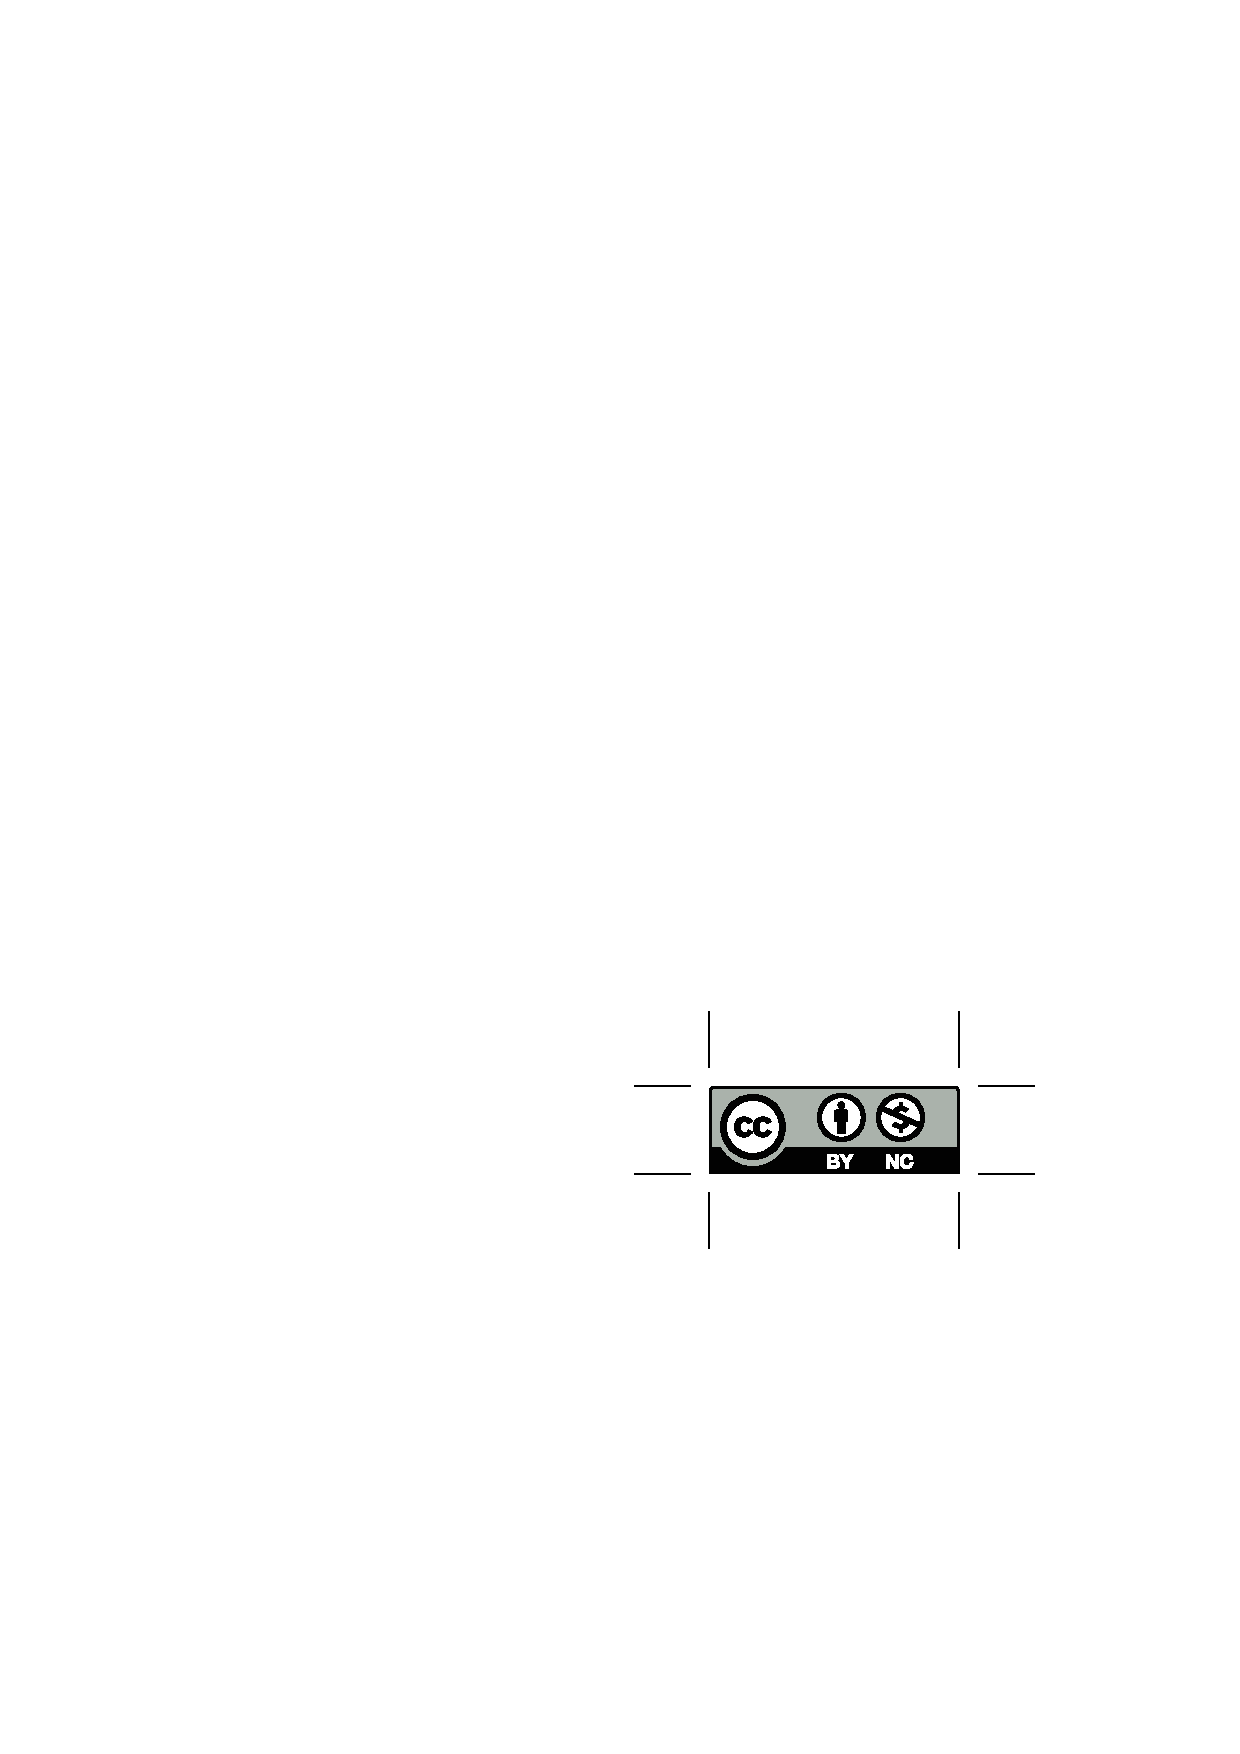
\includegraphics[width=2in]{text/by-nc} 
\end{center}
\end{minipage}
\begin{minipage}{3.3in}
Chapter 3 Copyright \copyright\ 2015 Gregory Hartman

Licensed under the Creative Commons Attribution-Noncommercial 4.0 International Public License
\end{minipage}

\bigskip

\bigskip

\bigskip

\noindent\hskip-1in\begin{minipage}{2.2in}
\begin{center}
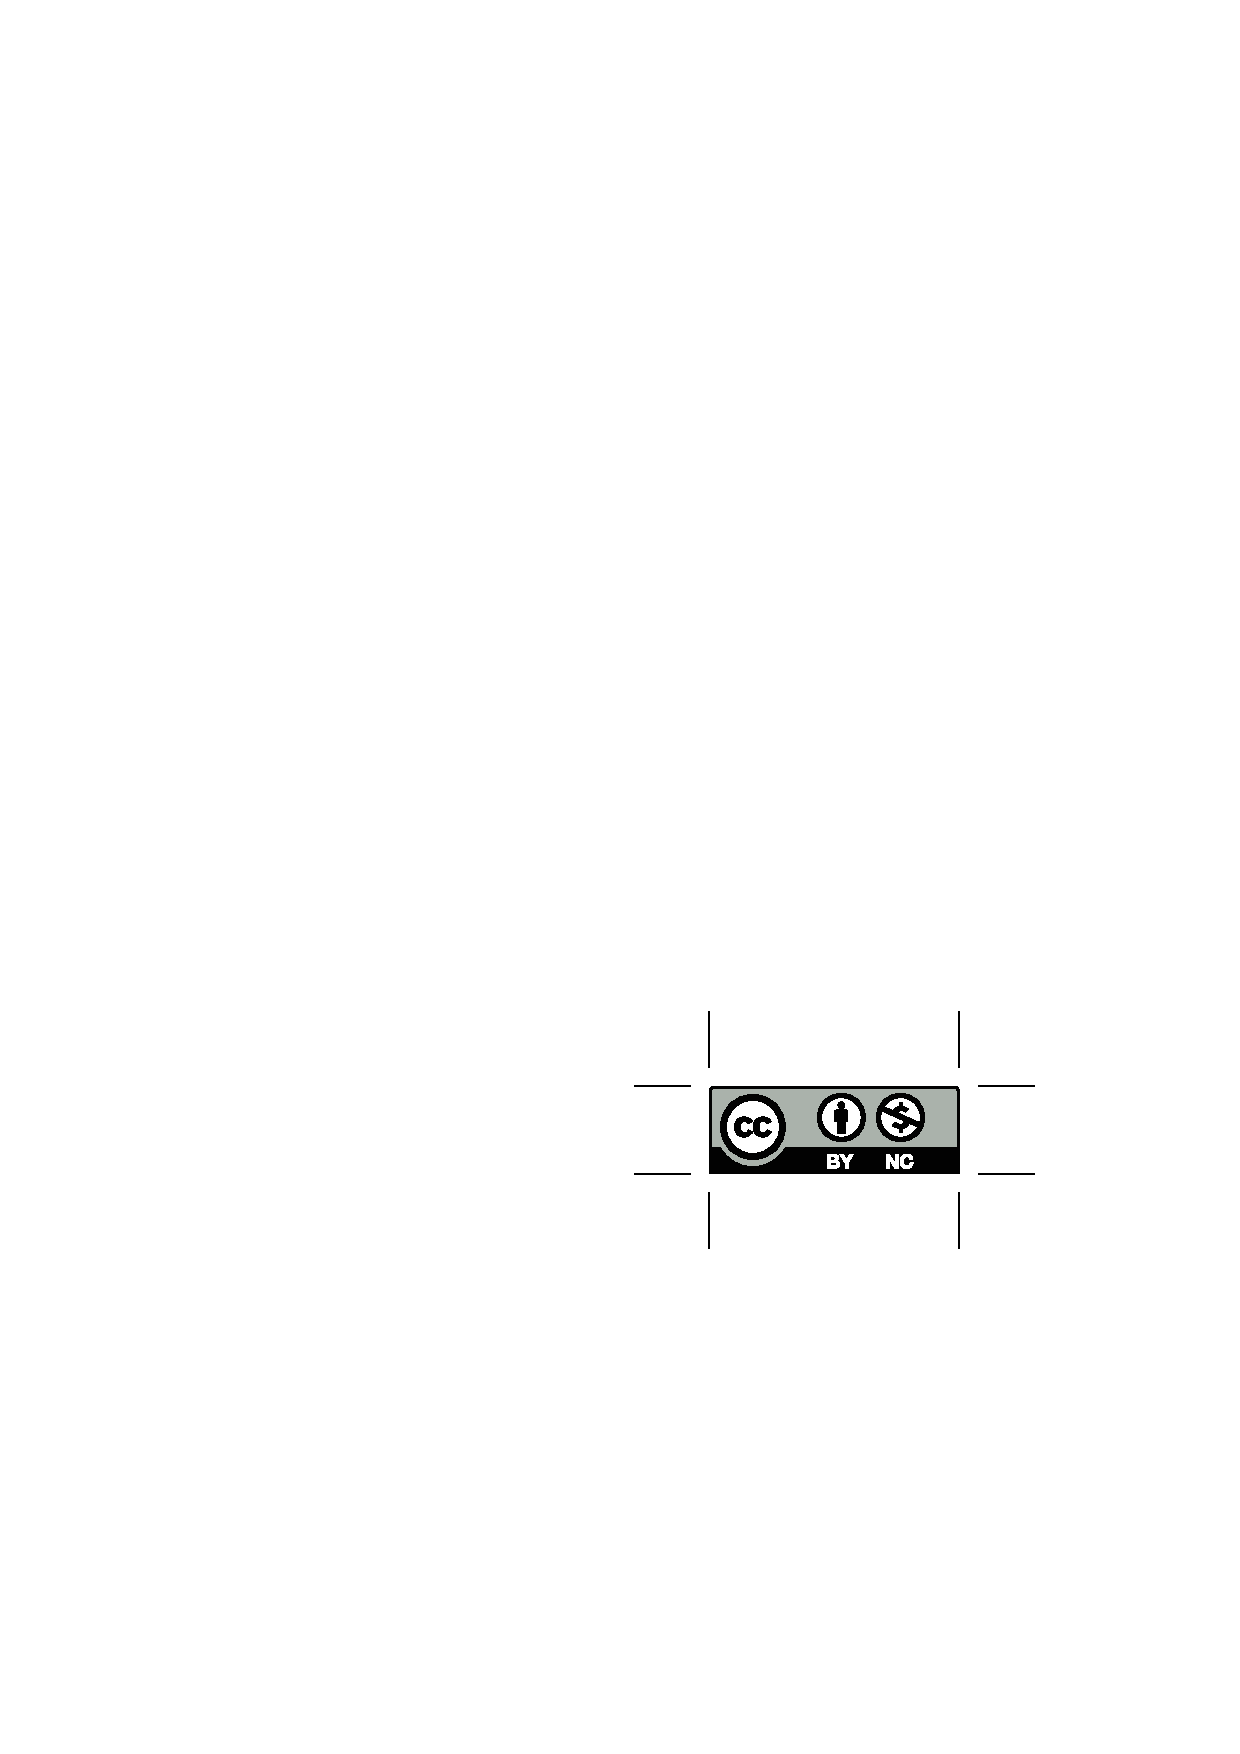
\includegraphics[width=2in]{text/by-nc}
\end{center}
\end{minipage}
\begin{minipage}{3.3in}
Chapters 4-8 Copyright \copyright\ 2011 Gregory Hartman, except as noted below.

Licensed under the Creative Commons Attribution-Noncommercial 3.0 United States License
\end{minipage}

\vspace{1in}


This version of the text was assembled and edited by Sean Fitzpatrick, University of Lethbridge, July-August, 2016. In addition to minor changes and additions throughout the text, supplementary content for this text was written by Sean Fitzpatrick, including all of Section 4.2, and parts of Sections 3.3-3.6, 4.1, 4.5, 6.1, 6.4, 7.4, and 8.1.

\medskip

This work is licensed under the Creative Commons Attribution-Noncommercial-ShareAlike 4.0 International Public License

\vspace{\stretch{1}} 
\thispagestyle{empty}
\clearpage


%\cleardoublepage
%%%%\phantomsection
%%%%\Huge
\noindent {\bf \textsc{Thanks}}\\

\vspace{1in}
\normalsize

This text took a great deal of effort to accomplish and I owe a great many people thanks. \\
\bigskip

I owe Michelle (and Sydney and Alex) much for their support at home. Michelle puts up with much as I continually read \LaTeX\ manuals, sketch outlines of the text, write exercises, and draw illustrations.\\

My thanks to the Department of Mathematics and Computer Science at Virginia Military Institute for their support of this project. Lee Dewald and Troy Siemers, my department heads, deserve special thanks for their special encouragement and recognition that this effort has been a worthwhile endeavor.\\

My thanks to all who informed me of errors in the text or provided ideas for improvement. Special thanks to Michelle Feole and Dan Joseph who each caught a number of errors.\\

This whole project would have been impossible save for the efforts of the \LaTeX\ community. This text makes use of about 15 different packages, was compiled using MiK\TeX, and edited using \TeX nicCenter, all of which was provided free of charge. This generosity helped convince me that this text should be made freely available as well.

\addtocontents{toc}{\protect\thispagestyle{empty}}
%%%%\addcontentsline{toc}{chapter}{Thanks} 
%%%%\clearpage{\pagestyle{empty}\cleardoublepage}
%%%%\phantomsection
%%%%\thispagestyle{empty}
\Huge
\noindent {\bf \textsc{Preface}}\\
\large
\emph{A Note on Using this Text}
\vspace{1in}
\normalsize

Thank you for reading this short preface. Allow us to share a few key points about the text so that you may better understand what you will find beyond this page.

This text comprises a three--volume series on Calculus. The first part covers material taught in many ``Calc 1'' courses: limits, derivatives, and the basics of integration, found in Chapters 1 through 6.1. The second text covers material often taught in ``Calc 2:'' integration and its applications, along with an introduction to sequences, series and Taylor Polynomials, found in Chapters 5 through 8. The third text covers topics common in ``Calc 3'' or ``multivariable calc:'' parametric equations, polar coordinates, vector--valued functions, and functions of more than one variable, found in Chapters 9 through 13. All three are available separately for free at \texttt{\href{http://apexcalculus.com}{www.apexcalculus.com}}. %These three texts are intended to work together and make one cohesive text, \textit{APEX Calculus}, which can also be downloaded from the website. 

Printing the entire text as one volume makes for a large, heavy, cumbersome book. One can certainly only print the pages they currently need, but some prefer to have a nice, bound copy of the text. Therefore this text has been split into these three manageable parts, each of which can be purchased for under \$15 at \href{http://amazon.com}{Amazon.com}.\\ 



%A result of this splitting is that sometimes a concept is said to be explored in a ``later section,'' though that section does not actually appear in this particular text. Downloading the .pdf of \textit{APEX Calculus} will ensure that you have all the content.  
%material is referenced that is not contained in the present text. The context should make it clear whether the ``missing'' material is in the \textit{Calculus I} or \textit{Calculus III} portion. Downloading the appropriate .pdf, or the whole \textit{APEX Calculus} .pdf, will give access to these topics.
% This splitting of the material also results in unfortunate page/chapter numberings. Chapter 5 of this text is Chapter 1 of \textit{Calculus II}. Apart from these numberings, page--for--page the content of the sections that appear in both \textit{Calculus I} and \textit{Calculus II} are identical.\\ %For instance, in this text, ``Theorem 20'' may be mentioned, although Theorem 20 is only presented in Part I. To minimize confusion, theorems, definitions and key ideas are referenced by their title or subject matter, not their number.

%The current publisher of this text does not allow one text to be split across multiple volumes, with continuity of chapters and page numberings. This is the one drawback of the current publishing model that has many advantages, highlighted below. Because of this, there are a few peculiarities 

\noindent\textbf{\large For Students: How to Read this Text}\\

Mathematics textbooks have a reputation for being hard to read. High--level mathematical writing often seeks to say much with few words, and this style often seeps into texts of lower--level topics. This book was written with the goal of being easier to read than many other calculus textbooks, without becoming too verbose. 

Each chapter and section starts with an introduction of the coming material, hopefully setting the stage for ``why you should care,'' and ends with a look ahead to see how the just--learned material helps address future problems. 

\textit{Please read the text;} it is written to explain the concepts of Calculus. There are numerous examples to demonstrate the meaning of definitions, the truth of theorems, and the application of mathematical techniques. When you encounter a sentence you don't understand, read it again. If it still doesn't make sense, read on anyway, as sometimes confusing sentences are explained by later sentences.

\textit{You don't have to read every equation.} The examples generally show ``all'' the steps needed to solve a problem. Sometimes reading through each step is helpful; sometimes it is confusing. When the steps are illustrating a new technique, one probably should follow each step closely to learn the new technique. When the steps are showing the mathematics needed to find a number to be used later, one can usually skip ahead and see how that number is being used, instead of getting bogged down in reading how the number was found.

\textit{Most proofs have been omitted.} In mathematics, \textit{proving} something is always true is extremely important, and entails much more than testing to see if it works twice. However, students often are confused by the details of a proof, or become concerned that they should have been able to construct this proof on their own. To alleviate this potential problem, we do not include the proofs to most theorems in the text. The interested reader is highly encouraged to find proofs online or from their instructor. In most cases, one is very capable of understanding what a theorem \textit{means} and \textit{how to apply it} without knowing fully \textit{why} it is true.
\\

\thispagestyle{empty}
\noindent\textbf{\large Interactive, 3D Graphics}\\

New to Version 3.0 is the addition of interactive, 3D graphics in the .pdf version. Nearly all graphs of objects in space can be rotated, shifted, and zoomed in/out so the reader can better understand the object illustrated. 

As of this writing, the only pdf viewers that support these 3D graphics are Adobe Reader \& Acrobat (and only the versions for PC/Mac/Unix/Linux computers, not tablets or smartphones). To activate the interactive mode, click on the image. Once activated, one can click/drag to rotate the object and use the scroll wheel on a mouse to zoom in/out. (A great way to investigate an image is to first zoom in on the page of the pdf viewer so the graphic itself takes up much of the screen, then zoom inside the graphic itself.) A CTRL-click/drag pans the object left/right or up/down. By right-clicking on the graph one can access a menu of other options, such as changing the lighting scheme or perspective. One can also revert the graph back to its default view. If you wish to deactive the interactivity, one can right-click and choose the ``Disable Content'' option. \\

\noindent\textbf{\large Thanks}\\

There are many people who deserve recognition for the important role they have played in the development of this text. First, I thank Michelle for her support and encouragement, even as this ``project from work'' occupied my time and attention at home. Many thanks to Troy Siemers, whose most important contributions extend far beyond the sections he wrote or the 227 figures he coded in Asymptote for 3D interaction.  He provided incredible support, advice and encouragement for which I am very grateful. My thanks to Brian Heinold and Dimplekumar Chalishajar for their contributions and to Jennifer Bowen for reading through so much material and providing great feedback early on. Thanks to Troy, Lee Dewald, Dan Joseph, Meagan Herald, Bill Lowe, John David, Vonda Walsh, Geoff Cox, Jessica Libertini and other faculty of VMI who have given me numerous suggestions and corrections based on their experience with teaching from the text. (Special thanks to Troy, Lee \& Dan for their patience in teaching Calc III while I was still writing the Calc III material.) Thanks to Randy Cone for encouraging his tutors of VMI's Open Math Lab to read through the text and check the solutions, and thanks to the tutors for spending their time doing so. A very special thanks to Kristi Brown and Paul Janiczek who took this opportunity far above \& beyond what I expected, meticulously checking every solution and carefully reading every example. Their comments have been extraordinarily helpful. I am also thankful for the support provided by Wane Schneiter, who as my Dean provided me with extra time to work on this project. I am blessed to have so many people give of their time to make this book better.\\

\noindent\textbf{\large \apex\  -- Affordable Print and Electronic teXts}\\

\apex\ is a consortium of authors  who collaborate to produce high--quality, low--cost textbooks. The current textbook--writing paradigm is facing a potential revolution as desktop publishing and electronic formats increase in popularity. However, writing a good textbook is no easy task, as the time requirements alone are substantial. It takes countless hours of work to produce text, write examples and exercises, edit and publish. Through collaboration, however, the cost to any individual can be lessened, allowing us to create texts that we freely distribute electronically and sell in printed form for an incredibly low cost. Having said that, nothing is entirely free; someone always bears some cost. This text ``cost'' the authors of this book their time, and that was not enough. \textit{APEX Calculus} would not exist had not the Virginia Military Institute, through a generous Jackson--Hope grant, given the lead author significant time away from teaching so he could focus on this text.

Each text is available as a free .pdf, protected by a Creative Commons Attribution - Noncommercial 4.0 copyright. That  means you can give the .pdf to anyone you like, print it in any form you like, and even edit the original content and redistribute it. If you do the latter, you must  clearly reference this work and you cannot sell your edited work for money.

We encourage others to adapt this work to fit their own needs. One might add sections that are ``missing'' or remove sections that your students won't need. The source files can be found at \texttt{\href{https://github.com/APEXCalculus}{github.com/APEXCalculus}}.

You can learn more at \texttt{\href{http://www.vmi.edu/APEX}{www.vmi.edu/APEX}}.
\thispagestyle{empty}


%%%%\addcontentsline{toc}{chapter}{Preface}
%%%%\clearpage{\pagestyle{empty}\cleardoublepage}
%%%%\phantomsection
%%%%

\addcontentsline{toc}{chapter}{Table of Contents}
\tableofcontents
\clearpage{\pagestyle{empty}\cleardoublepage}

\phantomsection
\prefacegeometry
\addcontentsline{toc}{chapter}{Preface}
\thispagestyle{empty}
\Huge
\noindent {\bf \textsc{Preface}}\\
\large
\emph{A Note on Using this Text}
\vskip 2\baselineskip
\normalsize

Thank you for reading this short preface. Allow us to share a few key points about the text so that you may better understand what you will find beyond this page.

This text is Part III of a three--text series on Calculus. The first part covers material taught in many ``Calc 1'' courses: limits, derivatives, and the basics of integration, found in Chapters 1 through 6.1. The second text covers material often taught in ``Calc 2:'' integration and its applications, along with an introduction to sequences, series and Taylor Polynomials, found in Chapters 5 through 8. The third text covers topics common in ``Calc 3'' or ``multivariable calc:'' parametric equations, polar coordinates, vector--valued functions, and functions of more than one variable, found in Chapters 9 through 13. All three are available separately for free at \texttt{\href{http://www.vmi.edu/APEX}{www.vmi.edu/APEX}}. These three texts are intended to work together and make one cohesive text, \textit{APEX Calculus}, which can also be downloaded from the website. 

Printing the entire text as one volume makes for a large, heavy, cumbersome book. One can certainly only print the pages they currently need, but some prefer to have a nice, bound copy of the text. Therefore this text has been split into these three manageable parts, each of which can be purchased for under \$15 at \href{http://amazon.com}{Amazon.com}. 

A result of this splitting is that sometimes a concept is said to be explored in an ``earlier section,'' though that section does not actually appear in this particular text. Also, the index makes reference to topics, and page numbers, that do not appear in this text. This is done intentionally to show the reader what topics are available for study.  Downloading the .pdf of \textit{APEX Calculus} will ensure that you have all the content.\\ 
%material is referenced that is not contained in the present text. The context should make it clear whether the ``missing'' material is in the \textit{Calculus I} or \textit{Calculus III} portion. Downloading the appropriate .pdf, or the whole \textit{APEX Calculus} .pdf, will give access to these topics.
  %For instance, in this text, ``Theorem 20'' may be mentioned, although Theorem 20 is only presented in Part I. To minimize confusion, theorems, definitions and key ideas are referenced by their title or subject matter, not their number.

%The current publisher of this text does not allow one text to be split across multiple volumes, with continuity of chapters and page numberings. This is the one drawback of the current publishing model that has many advantages, highlighted below. Because of this, there are a few peculiarities 

\noindent\textbf{\large For Students: How to Read this Text}\\

Mathematics textbooks have a reputation for being hard to read. High--level mathematical writing often seeks to say much with few words, and this style often seeps into texts of lower--level topics. This book was written with the goal of being easier to read than many other calculus textbooks, without becoming too verbose. 

Each chapter and section starts with an introduction of the coming material, hopefully setting the stage for ``why you should care,'' and ends with a look ahead to see how the just--learned material helps address future problems. 

\textit{Please read the text;} it is written to explain the concepts of Calculus. There are numerous examples to demonstrate the meaning of definitions, the truth of theorems, and the application of mathematical techniques. When you encounter a sentence you don't understand, read it again. If it still doesn't make sense, read on anyway, as sometimes confusing sentences are explained by later sentences.

\textit{You don't have to read every equation.} The examples generally show ``all'' the steps needed to solve a problem. Sometimes reading through each step is helpful; sometimes it is confusing. When the steps are illustrating a new technique, one probably should follow each step closely to learn the new technique. When the steps are showing the mathematics needed to find a number to be used later, one can usually skip ahead and see how that number is being used, instead of getting bogged down in reading how the number was found.

\textit{Most proofs have been omitted.} In mathematics, \textit{proving} something is always true is extremely important, and entails much more than testing to see if it works twice. However, students often are confused by the details of a proof, or become concerned that they should have been able to construct this proof on their own. To alleviate this potential problem, we do not include the proofs to most theorems in the text. The interested reader is highly encouraged to find proofs online or from their instructor. In most cases, one is very capable of understanding what a theorem \textit{means} and \textit{how to apply it} without knowing fully \textit{why} it is true.
\\

\thispagestyle{empty}
\noindent\textbf{\large Interactive, 3D Graphics}\\

New to Version 3.0 is the addition of interactive, 3D graphics in the .pdf version. Nearly all graphs of objects in space can be rotated, shifted, and zoomed in/out so the reader can better understand the object illustrated. 

As of this writing, the only pdf viewers that support these 3D graphics are Adobe Reader \& Acrobat (and only the versions for PC/Mac/Unix/Linux computers, not tablets or smartphones). To activate the interactive mode, click on the image. Once activated, one can click/drag to rotate the object and use the scroll wheel on a mouse to zoom in/out. (A great way to investigate an image is to first zoom in on the page of the pdf viewer so the graphic itself takes up much of the screen, then zoom inside the graphic itself.) A CTRL-click/drag pans the object left/right or up/down. By right-clicking on the graph one can access a menu of other options, such as changing the lighting scheme or perspective. One can also revert the graph back to its default view. If you wish to deactive the interactivity, one can right-click and choose the ``Disable Content'' option. \\

\noindent\textbf{\large Thanks}\\

There are many people who deserve recognition for the important role they have played in the development of this text. First, I thank Michelle for her support and encouragement, even as this ``project from work'' occupied my time and attention at home. Many thanks to Troy Siemers, whose most important contributions extend far beyond the sections he wrote or the 227 figures he coded in Asymptote for 3D interaction.  He provided incredible support, advice and encouragement for which I am very grateful. My thanks to Brian Heinold and Dimplekumar Chalishajar for their contributions and to Jennifer Bowen for reading through so much material and providing great feedback early on. Thanks to Troy, Lee Dewald, Dan Joseph, Meagan Herald, Bill Lowe, John David, Vonda Walsh, Geoff Cox, Jessica Libertini and other faculty of VMI who have given me numerous suggestions and corrections based on their experience with teaching from the text. (Special thanks to Troy, Lee \& Dan for their patience in teaching Calc III while I was still writing the Calc III material.) Thanks to Randy Cone for encouraging his tutors of VMI's Open Math Lab to read through the text and check the solutions, and thanks to the tutors for spending their time doing so. A very special thanks to Kristi Brown and Paul Janiczek who took this opportunity far above \& beyond what I expected, meticulously checking every solution and carefully reading every example. Their comments have been extraordinarily helpful. I am also thankful for the support provided by Wane Schneiter, who as my Dean provided me with extra time to work on this project. I am blessed to have so many people give of their time to make this book better.\\

\clearpage
\noindent\textbf{\large \apex\  -- Affordable Print and Electronic teXts}\\

\apex\ is a consortium of authors  who collaborate to produce high--quality, low--cost textbooks. The current textbook--writing paradigm is facing a potential revolution as desktop publishing and electronic formats increase in popularity. However, writing a good textbook is no easy task, as the time requirements alone are substantial. It takes countless hours of work to produce text, write examples and exercises, edit and publish. Through collaboration, however, the cost to any individual can be lessened, allowing us to create texts that we freely distribute electronically and sell in printed form for an incredibly low cost. Having said that, nothing is entirely free; someone always bears some cost. This text ``cost'' the authors of this book their time, and that was not enough. \textit{APEX Calculus} would not exist had not the Virginia Military Institute, through a generous Jackson--Hope grant, given the lead author significant time away from teaching so he could focus on this text.

Each text is available as a free .pdf, protected by a Creative Commons Attribution - Noncommercial 4.0 copyright. That  means you can give the .pdf to anyone you like, print it in any form you like, and even edit the original content and redistribute it. If you do the latter, you must  clearly reference this work and you cannot sell your edited work for money.

We encourage others to adapt this work to fit their own needs. One might add sections that are ``missing'' or remove sections that your students won't need. The source files can be found at \texttt{\href{https://github.com/APEXCalculus}{github.com/APEXCalculus}}.

You can learn more at \texttt{\href{http://www.vmi.edu/APEX}{www.vmi.edu/APEX}}.
\thispagestyle{empty}


\restoregeometry
\clearpage{\pagestyle{empty}\cleardoublepage}

%%%%
\mainmatter


%%%%
%		End block comment here
%%%%








%\chapter{Limits}\label{chapter:limits}
%\ifthenelse{\boolean{longpage}}{}{\thispagestyle{empty}}
%%
%\input{text/01_Limit_Introduction}
%\input{text/01_Limit_Definition}
%\input{text/01_Analytic_Limits}
%\input{text/01_One_Sided_Limits}
%\input{text/01_Continuity}
%\input{text/01_Limits_Involving_Infinity}


%%%\addtocounter{chapter}{1}
%
%\clearpage{\pagestyle{empty}\cleardoublepage}
%\chapter{Derivatives}\label{chapter:derivatives}
%\thispagestyle{empty}
%
%\input{text/02_Derivative}
%\input{text/02_Derivative_Meaning}
%\input{text/02_Derivative_Rules}
%\input{text/02_Product_Quotient_Rules}
%\input{text/02_Chain_Rule}
%\input{text/02_Implicit_Differentiation}
%\input{text/02_Derivative_Inverse_Functions}

%%\addtocounter{chapter}{2}

%\clearpage{\pagestyle{empty}\cleardoublepage}
%\chapter{The Graphical Behavior of Functions}\label{chapter:graphbehavior}
%\thispagestyle{empty}
%
%\input{text/03_Extreme_Values}
%\input{text/03_Mean_Value_Theorem}
%\input{text/03_Increasing_Decreasing}
%\input{text/03_Concavity}
%\input{text/03_Curve_Sketching}

%%\addtocounter{chapter}{3}
%
%\clearpage{\pagestyle{empty}\cleardoublepage}
%\chapter{Applications of the Derivative}\label{chapter:deriv_apps}
%\thispagestyle{empty}
%
%\input{text/04_NewtonsMethod}
%\input{text/04_Related_Rates}
%\input{text/04_Optimization}
%\input{text/04_Differentials}


%\addtocounter{chapter}{5}

%\clearpage{\pagestyle{empty}\cleardoublepage}

%\setcounterref{definitioncounter}{lastdefcount1}
%\addtocounter{definitioncounter}{-1}
%\setcounterref{theoremcounter}{lastthmcount1}
%\addtocounter{theoremcounter}{-1}
%\setcounterref{keyideacounter}{lastideacount1}
%\addtocounter{keyideacounter}{-1}
%\setcounterref{examplecounter}{lastexamplecount1}
%\addtocounter{examplecounter}{-1}
%\setcounter{page}{189}
%\thispagestyle{empty}

%\chapter{Integration}\label{chapter:integration}
%\addtocontents{toc}{\protect\enlargethispage{2\baselineskip}}
%\thispagestyle{empty}
%\setcounterpageref{page}{lastdefcount1}
%\addtocounter{page}{4}
%\input{text/05_Antiderivatives}
%\addtocontents{toc}{\protect\thispagestyle{empty}}
%\input{text/05_Definite_Integral}
%\input{text/05_Riemann_Sums}
%\input{text/05_FTC}
%\input{text/05_Numerical_Integration}


%%\addtocounter{chapter}{5}

%\clearpage{\pagestyle{empty}\cleardoublepage}
%\chapter{Techniques of Antidifferentiation}\label{chapter:anti_tech}
%\thispagestyle{empty}

%\input{text/06_Substitution}
%\input{text/06_Int_By_Parts}
%\input{text/06_Trigonometric_Integrals}
%\input{text/06_Trig_Sub}
%\input{text/06_Partial_Fractions}
%\input{text/06_Hyperbolic_Functions}
%\input{text/06_LHopitals_Rule}
%\input{text/06_Improper_Integration}

%%\addtocounter{chapter}{6}

%\clearpage{\pagestyle{empty}\cleardoublepage}
%\chapter{Applications of Integration}\label{chapter:app_of_int}
%\thispagestyle{empty}

%\input{text/07_Area_Between_Curves}
%\input{text/07_Disk_Washer_Method}
%\input{text/07_Shell_Method}
%\input{text/07_Arc_Length}
%\input{text/07_Work}
%\input{text/07_Fluid_Force}
\clearpage{\pagestyle{empty}\cleardoublepage}
\maketitle

\tableofcontents

\begin{quote}
This text is the based on the chapter on vectors from the APEX Calculus textbook by Hartman et al (www.apexcalculus.com) and compiled in this form by Sean Fitzpatrick.

\bigskip

Since this material originated in a Calculus textbook, some of the emphasis and notation will differ from your Linear Algebra textbook; however, most of the material here is covered in Math 1410, and it shouldn't be too difficult to make the connections between this text and the course textbook.

\bigskip

If you read this text using Adobe Reader, you should be able to interact with all of the 3D graphics in the text. This may be of help as you attempt to visualize lines and planes in three dimensions.
\end{quote}
\thispagestyle{empty}

%%\addtocounter{chapter}{7}

%
%%%\addtocounter{chapter}{9}
\clearpage{\pagestyle{empty}\cleardoublepage}
\chapter{Vectors}
\thispagestyle{empty}
%\input{text/10_Space_Intro_1410}
\section{An Introduction to Vectors}\label{sec:vector_intro}

Many quantities we think about daily can be described by a single number: temperature, speed, cost, weight and height. There are also many other concepts we encounter daily that cannot be described with just one number. For instance, a weather forecaster often describes wind with its speed and its direction (``$\ldots$ with winds from the south-east gusting up to 30 mph $\ldots$''). When applying a force, we are concerned with both the magnitude and direction of that force. In both of these examples, \textit{direction} is important. Because of this, we study \textit{vectors}, mathematical objects that convey both magnitude and direction information.\\

One ``bare--bones'' definition of a vector is based on what we wrote above: ``a vector is a mathematical object with magnitude and direction parameters.'' This definition leaves much to be desired, as it gives no indication as to how such an object is to be used. Several other definitions exist; we choose here a definition rooted in a geometric visualization of vectors. (In later chapters we will instead focus on algebraic aspects of vectors.) It is very simplistic but readily permits further investigation.

\definition{def:vector}{Vector}
{A \textbf{vector} is a directed line segment.\\

Given points $P$ and $Q$ (either in the plane or in space), we denote with $\overrightarrow{PQ}$ the vector \textit{from $P$ to $Q$}. The point $P$ is said to be the \textbf{initial point} of the vector, and the point $Q$ is the \textbf{terminal point}. \\

The \textbf{magnitude}, \textbf{length} or \textbf{norm} of $\overrightarrow{PQ}$ is the length of the line segment $\overline{PQ}$: $\norm{\overrightarrow{PQ}} = \norm{\overline{PQ}}$.\\

Two vectors are \textbf{equal} if they have the same magnitude and direction.
\index{vectors}\index{vectors!definition}\index{vectors!norm}\index{vectors!magnitude}\index{norm}\index{magnitude of vector}\index{terminal point}\index{initial point}
}

Figure \ref{fig:vectintro1} shows multiple instances of the same vector. Each directed line segment has the same direction and length (magnitude), hence each is the same vector.
\mfigure{.6}{Drawing the same vector with different initial points.}{fig:vectintro1}{figures/figvectintro1}

%Given two points $P$ and $Q$ (either in the plane or in space), the line segment that starts at $P$ and ends at $Q$ is a vector, denoted $\overrightarrow{PQ}$. The point $P$ is said to be the \textbf{initial} point of the vector, and the point $Q$ is the \textbf{terminal point}. We define the magnitude of $\overrightarrow{PQ}$ as the length of the line segment $\overline{PQ}$: $||\overrightarrow{PQ}|| = \norm{\overline{PQ}}$.

Following typical (but potentially confusing) mathematical convention, we use $\mathbb{R}^2$ (pronounced ``r two'') to represent all the vectors in the plane (as well as the plane itself), and use $\mathbb{R}^3$ (pronounced ``r three'') to represent all the vectors in space, as well as three-dimensional space itself.\index{r@$\mathbb{R}$}

\mfigure{.2}{Illustrating how equal vectors have the same displacement.}{fig:vectintro2}{figures/figvectintro2}
Consider the vectors $\overrightarrow{PQ}$ and $\overrightarrow{RS}$ as shown in Figure \ref{fig:vectintro2}. The vectors look to be equal; that is, they seem to have the same length and direction. Indeed, they are. Both vectors move 2 units to the right and 1 unit up from the initial point to reach the terminal point. One can analyze this movement to measure the magnitude of the vector, and the movement itself gives direction information (one could also measure the slope of the line passing through $P$ and $Q$ or $R$ and $S$). Since they have the same length and direction, these two vectors are equal.

This demonstrates that inherently all we care about is \textit{displacement}; that is, how far in the $x$, $y$ and possibly $z$ directions the terminal point is from the initial point. Both the vectors $\overrightarrow{PQ}$ and $\overrightarrow{RS}$ in Figure \ref{fig:vectintro2} have an $x$-displacement of 2 and a $y$-displacement of 1. This suggests a standard way of describing vectors in the plane. A vector whose $x$-displacement is $a$ and whose $y$-displacement is $b$ will have terminal point $(a,b)$ when the initial point is the origin, $(0,0)$. This leads us to a definition of a standard and concise way of referring to vectors.

\definition{def:vector_component}{Component Form of a Vector}
{\begin{enumerate}
	\item The \textbf{component form} of a vector $\vec{v}$ in $\mathbb{R}^2$, whose terminal point is $(a,b)$ when its initial point is $(0,0)$, is $\la a,b\ra.$ 
	
	\item	The \textbf{component form} of a vector $\vec{v}$ in $\mathbb{R}^3$, whose terminal point is $(a,b,c)$ when its initial point is $(0,0,0)$, is $\la a,b,c\ra.$ 
	
	%The component form of the vector $\overrightarrow{PQ}$, where $P=(x_1,y_1,z_1)$ and $Q=(x_2,y_2,z_2)$ is 
	%$$\overrightarrow{PQ} = \la x_2-x_1, y_2-y_1,z_2-z_1\ra.$$
\end{enumerate}
The numbers $a$, $b$ (and $c$, respectively) are the \textbf{components} of $\vec v$.
\index{vectors!component form}
}

\mnote{.82}{The component form of a vector allows us to identify a point $(a,b)$ (or $(a,b,c)$) with the corresponding vector $\langle a,b\rangle$ (or $\la a,b,c\ra$), so that vectors and points contain essentially the same information, presented in different contexts. This is why mathematicians don't mind using the notation $\mathbb{R}^n$ to refer to both a set of vectors and the set of points containing those vectors.}

\mnote{.65}{\textbf{Caution:} The notation $\la a,b,c\ra$ used in this chapter for a vector is common in geometry, physics, and calculus, but in later chapters we will use \textit{column vector} notation $\bbm a\\b\\c\ebm$ to represent the same vector. This notation is more natural in the context of matrix algebra.}


It follows from the definition that the component form of the vector $\overrightarrow{PQ}$, where $P=(x_1,y_1)$ and $Q=(x_2,y_2)$ is 
\[
\overrightarrow{PQ} = \la x_2-x_1, y_2-y_1\ra;
\]
in space, where $P=(x_1,y_1,z_1)$ and $Q=(x_2,y_2,z_2)$, the component form of $\overrightarrow{PQ}$ is	
\[
\overrightarrow{PQ} = \la x_2-x_1, y_2-y_1,z_2-z_1\ra.
\]
We practice using this notation in the following example.\\

\enlargethispage{2\baselineskip}

\example{ex_vect1}{Using component form notation for vectors}{
\begin{enumerate}
	\item Sketch the vector $\vec v=\la 2,-1\ra$ starting at $P=(3,2)$ and find its magnitude.
	\item		Find the component form of the vector $\vec w$ whose initial point is $R=(-3,-2)$ and whose terminal point is $S=(-1,2)$.
	\item	Sketch the vector $\vec u = \la 2,-1,3\ra$ starting at the point $Q = (1,1,1)$ and find its
magnitude.
\end{enumerate}
}
{\begin{enumerate}
	\item Using $P$ as the initial point, we move 2 units in the positive $x$-direction and $-1$ units in the positive $y$-direction to arrive at the terminal point $P\,'=(5,1)$, as drawn in Figure \ref{fig:vect1}(a).
	
	The magnitude of $\vec v$ is determined directly from the component form:
\[
\norm{\vec v} =\sqrt{2^2+(-1)^2} = \sqrt{5}. 
\]
	\mtable{.3}{Graphing vectors in Example \ref{ex_vect1}.}{fig:vect1}{%
	\begin{tabular}{c}
	\myincludegraphics{figures/figvectintro3}\\
	(a)\\[20pt]
	\myincludegraphicsthree{width=125pt,3Dmenu,activate=onclick,deactivate=onclick,
3Droll=0,
3Dortho=0.004,
3Dc2c=.3 .9 .3,
3Dcoo=49 42 58,
3Droo=150,
3Dlights=Headlamp,add3Djscript=asylabels.js}{scale=1.25,trim=5mm 5mm 5mm 5mm,clip=true}{figures/figvectintro3b}\\
%\myincludegraphics[scale=1.25,trim=5mm 5mm 5mm 5mm,clip=true]{figures/figvectintro3b}\\
	(b)
	\end{tabular}
	}
	
	\item		Using the note following Definition \ref{def:vector_component}, we have
\[
\overrightarrow{RS} = \la -1-(-3), 2-(-2)\ra = \la 2,4\ra.
\]
One can readily see from Figure \ref{fig:vect1}(a) that the $x$- and $y$-displacement of $\overrightarrow{RS}$ is 2 and 4, respectively, as the component form suggests.
	
	\item		Using $Q$ as the initial point, we move 2 units in the positive $x$-direction, $-1$ unit in the positive $y$-direction, and 3 units in the positive $z$-direction to arrive at the terminal point $Q' = (3,0,4)$, illustrated in Figure \ref{fig:vect1}(b).
	
	The magnitude of $\vec u$ is:
\[
\norm{\vec u} = \sqrt{2^2+(-1)^2+3^2} = \sqrt{14}.
\]
\end{enumerate}
\vskip-\baselineskip
}

\pagebreak

Now that we have defined vectors, and have created a nice notation by which to describe them, we start considering how vectors interact with each other. That is, we define an \textit{algebra} on vectors. 
%\clearpage

\definition{def:vector_algebra}{Vector Algebra}
{\begin{enumerate}
	\item Let $\vec u = \la u_1,u_2\ra$ and $\vec v = \la v_1,v_2\ra$ be vectors in $\mathbb{R}^2$, and let $c$ be a scalar. \index{vectors!algebra of}
				\begin{enumerate}
					\item The addition, or sum, of the vectors $\vec u$ and $\vec v$ is the vector
					\[
					\vec u+\vec v = \la u_1+v_1, u_2+v_2\ra.
					\]
					\item	The scalar product of $c$ and $\vec v$ is the vector 
					\[
					c\vec v = c\la v_1,v_2\ra = \la cv_1,cv_2\ra.
					\]
				\end{enumerate}
	\item Let $\vec u = \la u_1,u_2,u_3\ra$ and $\vec v = \la v_1,v_2,v_3\ra$ be vectors in $\mathbb{R}^3$, and let $c$ be a scalar. 
				\begin{enumerate}
					\item The addition, or sum, of the vectors $\vec u$ and $\vec v$ is the vector
					\[
					\vec u+\vec v = \la u_1+v_1, u_2+v_2, u_3+v_3\ra.
					\]
					\item	The scalar product of $c$ and $\vec v$ is the vector 
	\[
			c\vec v = c\la v_1,v_2,v_3\ra = \la cv_1,cv_2,cv_3\ra.
	\]
				\end{enumerate}
\end{enumerate}
}

In short, we say addition and scalar multiplication are computed ``component--wise.''\\

\example{ex_vect2}{Adding vectors}{
	Sketch the vectors $\vec u = \la1,3\ra$, $\vec v = \la 2,1\ra$ and $\vec u+\vec v$ all with initial point at the origin.}
	{We first compute $\vec u +\vec v$. 
	\begin{align*}
	\vec u+\vec v &= \la 1,3\ra + \la 2,1\ra\\
								&= \la 3,4\ra.
	\end{align*}
	\mfigure{.35}{Graphing the sum of vectors in Example \ref{ex_vect2}.}{fig:vect2}{figures/figvect2}
	These are all sketched in Figure \ref{fig:vect2}.
}\\
	
As vectors convey magnitude and direction information, the sum of vectors also convey length and magnitude information. Adding $\vec u+\vec v$ suggests the following idea:
\begin{quotation}
``Starting at an initial point, go out $\vec u$, then go out $\vec v$.''
\end{quotation}

This idea is sketched in Figure \ref{fig:vect2b}, where the initial point of $\vec v$ is the terminal point of $\vec u$. This is known as the ``Head to Tail Rule'' of adding vectors. Vector addition is very important. For instance, if the vectors $\vec u$ and $\vec v$ represent forces acting on a body, the sum $\vec u+\vec v$ gives the resulting force. Because of various physical applications of vector addition, the sum $\vec u+\vec v$ is often referred to as the \sword{resultant vector}, or just the ``resultant.''\index{vectors!resultant}\index{Parallelogram Law}\index{vectors!Parallelogram Law}\index{Head To Tail Rule}\index{vectors!Head To Tail Rule}\index{vectors!zero vector}

Analytically, it is easy to see that $\vec u+\vec v = \vec v+\vec u$. Figure \ref{fig:vect2b} also gives a graphical representation of this, using gray vectors. Note that the vectors $\vec u$ and $\vec v$, when arranged as in the figure, form a parallelogram. Because of this, the Head to Tail Rule is also known as the Parallelogram Law: the vector $\vec u+\vec v$ is defined by forming the parallelogram defined by the vectors $\vec u$ and $\vec v$; the initial point of $\vec u+\vec v$ is the common initial point of parallelogram, and the terminal point of the sum is the common terminal point of the parallelogram.

\mfigure{.75}{Illustrating how to add vectors using the Head to Tail Rule and Parallelogram Law.}{fig:vect2b}{figures/figvect2b}

While not illustrated here, the Head to Tail Rule and Parallelogram Law hold for vectors in $\mathbb{R}^3$ as well.

It follows from the properties of the real numbers and Definition \ref{def:vector_algebra} that 
\[
\vec u-\vec v = \vec u + (-1)\vec v.
\]
The Parallelogram Law gives us a good way to visualize this subtraction. We demonstrate this in the following example.\\

\example{ex_vect4}{Vector Subtraction}{
Let $\vec u = \la 3,1\ra$ and $\vec v=\la 1,2\ra.$ Compute and sketch $\vec u-\vec v$.
}
{The computation of $\vec u-\vec v$ is straightforward, and we show all steps below. Usually the formal step of multiplying by $(-1)$ is omitted and we ``just subtract.''
\begin{align*}
\vec u-\vec v &= \vec u + (-1)\vec v \\
							&= \la 3,1\ra + \la -1,-2\ra\\
							&= \la 2,-1\ra.
\end{align*}
\mfigure{.55}{Illustrating how to subtract vectors graphically.}{fig:vect4}{figures/figvect4}
Figure \ref{fig:vect4} illustrates, using the Head to Tail Rule, how the subtraction can be viewed as the  sum $\vec u + (-\vec v)$. The figure also illustrates how $\vec u-\vec v$ can be obtained by looking only at the terminal points of $\vec u$ and $\vec v$ (when their initial points are the same).
}\\

\enlargethispage{2\baselineskip}

\example{ex_vect3}{Scaling vectors}{
\begin{enumerate}
\item	Sketch the vectors $\vec v = \la 2,1\ra$ and  $2\vec v$ with initial point at the origin. 
\item Compute the magnitudes of $\vec v$ and $2\vec v$.
\end{enumerate}
}
{\begin{enumerate}
\item	We compute $2\vec v$:
	\begin{align*}
	2\vec v &= 2\la 2,1\ra\\
					&= \la 4,2\ra.
	\end{align*}
	\mfigure{.25}{Graphing vectors $\vec v$ and $2\vec v$ in Example \ref{ex_vect3}.}{fig:vect3}{figures/figvect3}
	Both $\vec v$ and $2\vec v$ are sketched in Figure \ref{fig:vect3}. Make note that $2\vec v$ does not start at the terminal point of $\vec v$; rather, its initial point is also the origin. 
	
\item		The figure suggests that $2\vec v$ is twice as long as $\vec v$. We compute their magnitudes to confirm this.
\begin{align*}
\norm{\vec v} &= \sqrt{2^2+1^2}\\
							&= \sqrt{5}.\\
\norm{2\vec v}&=\sqrt{4^2+2^2} \\
							&= \sqrt{20}\\
							&= \sqrt{4\cdot 5} = 2\sqrt{5}.
\end{align*}
As we suspected, $2\vec v$ is twice as long as $\vec v$.
\end{enumerate}
\vskip-\baselineskip
}

\pagebreak

In Example \ref{ex_vect3} above, we saw that $\len{2\vec v} = 2\len{\vec v}$, which makes sense geometrically: $2\vec v = \vec v+\vec v$, and adding a vector to itself should produce a vector twice as long with the same direction. The following theorem tells us that this is true in general.

\theorem{thm:vecscale}{Magnitude and scalar multiplication}{
For any vector $\vec v$ in $\R^2$ or $\R^3$, and any real number $c$, we have
\[
\len{c\vec v} = \abs{c}\len{\vec{v}}.
\]
}

In particular, Theorem \ref{thm:vecscale} tells us that if $c>0$, then $\len{c\vec{v}}=c\len{\vec{v}}$, so that $c\vec{v}$ is a vector in the \textit{same} direction as $\vec{v}$ whose magnitude has been stretched (if $c>1$) or shrunk (if $c<1$) by a factor of $c$ relative to that of $\vec{v}$. On the other hand, if $c<0$, then we have $\len{c\vec{v}}=-c\len{\vec{v}}$, so that $c\vec{v}$ points in the \textit{opposite} direction to that of $\vec{v}$.

\mnote{.7}{To prove Theorem \ref{thm:vecscale}, let $\vec{v}=\la a,b\ra$ be any vector in $\R^2$ (the proof for $\R^3$ is similar), and let $c$ be any scalar. Then
\begin{align*}
\len{c\vec{v}}  & = \len{c\la a,b\ra}\\
				& = \len{\la ca, cb\ra}\\
				& = \sqrt{(ca)^2+(cb)^2}\\
				& = \sqrt{c^2a^2+c^2b^2}\\
				& = \sqrt{c^2(a^2+b^2)}\\
				& = \sqrt{c^2}\sqrt{a^2+b^2}\\
				& = \abs{c}\len{\vec{v}},
\end{align*}
as required.\\
(Recall that $\sqrt{c^2}=\abs{c}$, the absolute value of $c$, since $c$ might be negative, but the square root is always positive.)}

The \textbf{zero vector} is the vector whose initial point is also its terminal point. It is denoted by $\vec 0$. Its component form, in $\mathbb{R}^2$, is $\la 0,0\ra$; in $\mathbb{R}^3$, it is $\la 0,0,0\ra$. Usually the context makes is clear whether $\vec 0$ is referring to a vector in the plane or in space.

Our examples have illustrated key principles in vector algebra: how to add and subtract vectors and how to multiply vectors by a scalar. The following theorem states formally the properties of these operations.
%\clearpage

\theorem{thm:vector_properties}{Properties of Vector Operations}
{The following are true for all scalars $c$ and $d$, and for all vectors $\vec u$, $\vec v$ and $\vec w$, where $\vec u$, $\vec v$ and $\vec w$ are all in $\mathbb{R}^2$ or where $\vec u$, $\vec v$ and $\vec w$ are all in $\mathbb{R}^3$:\index{vectors!algebraic properties}
\begin{enumerate}
	\item \parbox{150pt}{$\vec u+\vec v = \vec v+\vec u$}Commutative Property
	\item \parbox{150pt}{$(\vec u+\vec v)+\vec w = \vec u+(\vec v+\vec w)$}Associative Property
	\item \parbox{150pt}{$\vec v+\vec 0 = \vec v$}Additive Identity
	\item \parbox{150pt}{$(cd)\vec v= c(d\vec v)$}
	\item \parbox{150pt}{$c(\vec u+\vec v) = c\vec u+c\vec v$}Distributive Property
	\item \parbox{150pt}{$(c+d)\vec v = c\vec v+d\vec v$}Distributive Property
	\item \parbox{150pt}{$0\vec v = \vec 0$}
	\item	\parbox{150pt}{$\norm{c\vec v} = |c|\cdot\norm{\vec v}$}\label{thm:norm_prop}
	\item	$\vnorm u = 0$ if, and only if, $\vecu = \vec 0$.  \label{thm:zero_norm}
\end{enumerate}
}

%The result of the Example \ref{ex_vect3} leads us to the following theorem about multiplying vectors by a scalar.
%
%\theorem{thm:vector_scale}{Scaling Vectors}
%{Let $\vec v$ be a vector in $\mathbb{R}^2$ or $\mathbb{R^3}$ and let $c$ be a scalar. Then
%$$\norm{c\vec v} = |c|\cdot\norm{\vec v}.$$
%}

The verification of each of the properties in Theorem \ref{thm:vector_properties} is straightforward, and left as an exercises for the reader.

As stated before, each vector $\vec v$ conveys magnitude and direction information. We have a method of extracting the magnitude, which we write as $\norm{\vec v}$. \textit{Unit vectors} are a way of extracting just the direction information from a vector.

\definition{def:unit_vector}{Unit Vector}
{A \textbf{unit vector} is a vector $\vec v$ with a magnitude of 1; that is, 
\index{vectors!unit vector}\index{unit vector}
\[
\norm{\vec v}=1.
\]
}

Consider this scenario: you are given a vector $\vec v$ and are told to create a vector of length 10 in the direction of $\vec v$. How does one do that? If we knew that $\vec u$ was the unit vector in the direction of $\vec v$, the answer would be easy: $10\vec u$. So how do we find $\vec u$\,?

Property \ref{thm:norm_prop} of Theorem \ref{thm:vector_properties} holds the key. If we divide $\vec v$ by its magnitude, it becomes a vector of length 1. Consider:
\begin{align*}
\snorm{\frac{1}{\norm{\vec v}}\vec v} &= \frac{1}{\norm{\vec v}}\norm{\vec v} & \text{\small (we can pull out $\ds \frac{1}{\norm{\vec v}}$ as it is a scalar)}\\
								&= 1.
\end{align*}			
So the vector of length 10 in the direction of $\vec v$ is $\ds 10\frac{1}{\norm{\vec v}}\vec v.$ An example will make this more clear.\\

\example{ex_vect5}{Using Unit Vectors}{
Let $\vec v= \la 3,1\ra$ and let $\vec w = \la 1,2,2\ra$. 
\begin{enumerate}
	\item Find the unit vector in the direction of $\vec v$.
	\item	Find the unit vector in the direction of $\vec w$.
	\item	Find the vector in the direction of $\vec v$ with magnitude 5.
\end{enumerate}}
{\begin{enumerate}
	\item We find $\norm{\vec v} = \sqrt{10}$. So the unit vector $\vec u$ in the direction of $\vec v$ is 
	\[
	\vec u = \frac{1}{\sqrt{10}}\vec v = \la \frac{3}{\sqrt{10}},\frac{1}{\sqrt{10}}\ra.
	\]
	\item		We find $\norm{\vec w} = 3$, so the unit vector $\vec z$ in the direction of $\vec w$ is
	\[
	\vec u = \frac13\vec w = \la \frac13,\frac23,\frac23\ra.
	\]
	\item		To create a vector with magnitude 5 in the direction of $\vec v$, we multiply the unit vector $\vec u$ by 5. Thus $5\vec u = \la 15/\sqrt{10},5/\sqrt{10}\ra$ is the vector we seek. This is sketched in Figure \ref{fig:vect5}.
	\mfigure{.7}{Graphing vectors in Example \ref{ex_vect5}. All vectors shown have their initial point at the origin.}{fig:vect5}{figures/figvect5}
\end{enumerate}
\vskip-\baselineskip
}\\

The basic formation of the unit vector $\vec u$ in the direction of a vector $\vec v$ leads to a interesting equation. It is:
\[
\vec v = \norm{\vec v}\frac{1}{\norm{\vec v}}\vec v.
\]
We rewrite the equation with parentheses to make a point:
\[
\vec v = \underbrace{\rule[-9.5pt]{0pt}{15pt}\norm{\vec v}}_{\text{\scriptsize magnitude}}\cdot\underbrace{\left(\frac{1}{\norm{\vec v}}\vec v\right)}_{\text{\scriptsize direction}}.
\]

This equation illustrates the fact that a vector has both magnitude and direction, where we view a unit vector as supplying \textit{only} direction information. Identifying unit vectors with direction allows us to define \textbf{parallel vectors}.

\definition{def:parallel_vectors}{Parallel Vectors}
{\begin{enumerate}
	\item Unit vectors $\vec u_1$ and $\vec u_2$ are \textbf{parallel} if $\vec u_1 = \pm \vec u_2$.
	\index{vectors!parallel}\index{parallel vectors}
	\item	Nonzero vectors $\vec v_1$ and $\vec v_2$ are \textbf{parallel} if their respective unit vectors are parallel.
\end{enumerate}
}

It is equivalent to say that vectors $\vec v_1$ and $\vec v_2$ are parallel if there is a scalar $c\neq 0$ such that $\vec v_1 = c\vec v_2$ (see marginal note). 
\mnote{.7}{\textbf{Note:} $\vec 0$ is directionless; because $\vnorm{0}=0$, there is no unit vector in the ``direction'' of $\vec 0$. 

Some texts define two vectors as being parallel if one is a scalar multiple of the other. By this definition, $\vec 0$ is parallel to all vectors as $\vec 0 = 0\vec v$ for all $\vec v$.

For this chapter on vector \textit{geometry}, we will use Definition \ref{def:parallel_vectors} of parallel as it is grounded in the fact that unit vectors provide direction information. One may adopt the convention that $\vec 0$ is parallel to all vectors if they desire. (See also the marginal note on page \pageref{note:crossp}.)\label{note:parallel} In later chapters (once we move on to vector \textit{algebra}) it will be more convenient to say that a vector $\vec w$ is parallel to a given vector $\vec{v}$ if there exists a scalar $c$ such that $\vec w = c\vec v$.}

If one graphed all unit vectors in $\mathbb{R}^2$ with the initial point at the origin, then the terminal points would all lie on the unit circle $x^2+y^2=1$. Based on what we know from trigonometry, we can then say that the component form of all unit vectors in $\mathbb{R}^2$ is $\la \cos\theta,\sin\theta\ra$ for some angle $\theta$.

A similar construction in $\mathbb{R}^3$ shows that the terminal points all lie on the unit sphere $x^2+y^2+z^2=1$. These vectors also have a particular component form, but its derivation is not as straightforward as the one for unit vectors in $\mathbb{R}^2$. Important concepts about unit vectors are given in the  following Key Idea. 

\keyidea{idea:unit_vectors}{Unit Vectors}
{\begin{enumerate}
\item		The unit vector in the direction of $\vec v$ is 
\[
 \vec u = \frac1{\norm{\vec v}} \vec v.
\]

\item A vector $\vec u$ in $\mathbb{R}^2$ is a unit vector if, and only if, its component form is $\la \cos\theta,\sin\theta\ra$ for some angle $\theta$.
\index{unit vector!properties}\index{vectors!unit vector}
	\item		A vector $\vec u$ in $\mathbb{R}^3$ is a unit vector if, and only if, its component form is $\la \sin\theta\cos\varphi,\sin\theta\sin\varphi,\cos\theta\ra$ for some angles $\theta$ and $\varphi$.
\end{enumerate}
}

These formulas can come in handy in a variety of situations, especially the formula for unit vectors in the plane.\\

\mnote{.4}{\textbf{Note:} the component form given in Key Idea \ref{idea:unit_vectors} for a unit vector in $\R^3$ is derived from the \href{https://en.wikipedia.org/wiki/Spherical_coordinate_system}{\underline{spherical coordinate system}} for $\R^3$.}

\example{ex_vect6}{Finding Component Forces}{
Consider a weight of 50lb hanging from two chains, as shown in Figure \ref{fig:vect6}. One chain makes an angle of $30^\circ$ with the vertical, and the other an angle of $45^\circ$. Find the force applied to each chain.
\mfigure{.2}{A diagram of a weight hanging from 2 chains in Example \ref{ex_vect6}.}{fig:vect6}{figures/figvect6}}
{Knowing that gravity is pulling the 50lb weight straight down, we can create a vector $\vec F$ to represent this force. 
\[
\vec F = 50\la 0,-1\ra = \la 0,-50\ra.
\]

We can view each chain as ``pulling'' the weight up, preventing it from falling. We can represent the force from each chain with a vector. Let $\vec F_1$ represent the force from the chain making an angle of $30^\circ$ with the vertical, and let $\vec F_2$ represent the force form the other chain. Convert all angles to be measured from the horizontal (as shown in Figure \ref{fig:vect6b}), and apply Key Idea \ref{idea:unit_vectors}. As we do not yet know the magnitudes of these vectors, (that is the problem at hand), we use $m_1$ and $m_2$ to represent them.
\begin{align*}
\vec F_1 &= m_1\la \cos 120^\circ,\sin120^\circ\ra\\
\vec F_2 &= m_2\la \cos 45^\circ,\sin45^\circ\ra
\end{align*}
As the weight is not moving, we know the sum of the forces is $\vec 0$. This gives:
\begin{align*}
\vec 0 & = \vec F + \vec F_1 + \vec F_2 \\
& = \la 0,-50\ra + m_1\la \cos 120^\circ,\sin120^\circ\ra + m_2\la \cos 45^\circ,\sin45^\circ\ra 
\end{align*}

\mfigure{.8}{A diagram of the force vectors from Example \ref{ex_vect6}.}{fig:vect6b}{figures/figvect6b}
The sum of the entries in the first component is 0, and the sum of the entries in the second component is also 0. This leads us to the following two equations:
\begin{align*}
m_1\cos120^\circ + m_2\cos45^\circ &=0 \\
m_1\sin120^\circ + m_2\sin45^\circ &=50
\end{align*}
This is a simple 2-equation, 2-unknown system of linear equations. We leave it to the reader to verify that the solution is 
\[
m_1=50(\sqrt{3}-1) \approx 36.6;\qquad m_2=\frac{50\sqrt{2}}{1+\sqrt{3}} \approx 25.88.
\]

It might seem odd that the sum of the forces applied to the chains is more than 50lb. We leave it to a physics class to discuss the full details, but offer this short explanation. Our equations were established so that the \textit{vertical} components of each force sums to 50lb, thus supporting the weight. Since the chains are at an angle, they also pull against each other, creating an ``additional'' horizontal force while holding the weight in place.
}\\

Unit vectors were very important in the previous calculation; they allowed us to define a vector in the proper direction but with an unknown magnitude. Our computations were then computed component--wise. Because such calculations are often necessary, the \textit{standard unit vectors} can be useful.

\definition{def:standard_unit}{Standard Unit Vectors}
{\begin{enumerate}
	\item In $\mathbb{R}^2$, the standard unit vectors are
	\index{vectors!standard unit vector}\index{unit vector!standard unit vector}
	\[
	\vec i = \la 1,0\ra \quad \text{and}\quad \vec j = \la 0,1\ra.
	\]
	\item In $\mathbb{R}^3$, the standard unit vectors are
	\[
	\vec i = \la 1,0,0\ra \quad \text{and}\quad \vec j = \la 0,1,0\ra \quad \text{and}\quad \vec k = \la 0,0,1\ra.
	\]
\end{enumerate}
}

\example{ex_vect7}{Using standard unit vectors}{
\begin{enumerate}
	\item Rewrite $\vec v = \la 2,-3\ra$ using the standard unit vectors.
	\item	Rewrite $\vec w = 4\vec i - 5\vec j +2\vec k$ in component form.
\end{enumerate}\pagebreak
}
{\begin{enumerate}
	\item  \hfill$\displaystyle \begin{aligned}[t]
					\vec v &= \la 2,-3\ra \\
								&= \la 2,0\ra + \la 0,-3\ra \\
								&= 2\la 1,0\ra -3\la 0,1\ra\\
								&= 2\vec i - 3\vec j
				\end{aligned}$\hfill\null
	
	\item	\hfill $\displaystyle \begin{aligned}[t]
				\vec w &= 4\vec i - 5\vec j +2\vec k\\
							&= \la 4,0,0\ra +\la 0,-5,0\ra + \la 0,0,2\ra \\
							&= \la 4,-5,2\ra
							\end{aligned}$\hfill\null
\end{enumerate}
These two examples demonstrate that converting between component form and the standard unit vectors is rather straightforward. Many mathematicians prefer component form, and it is the preferred notation in this text. Many engineers prefer using the standard unit vectors, and many engineering texts use that notation.
}\\

\example{ex_vect8}{Finding Component Force}{
A weight of 25lb is suspended from a chain of length 2ft while a wind pushes the weight to the right with constant force of 5lb as shown in Figure \ref{fig:vect8}. What angle will the chain make with the vertical as a result of the wind's pushing? How much higher will the weight be?
\mfigure{.5}{A figure of a weight being pushed by the wind in Example \ref{ex_vect8}.}{fig:vect8}{figures/figvect8}
}
{The force of the wind is represented by the vector $\vec F_w = 5\vec i$. The force of gravity on the weight is represented by $\vec F_g = -25\vec j$. The direction and magnitude of the vector representing the force on the chain are both unknown. We represent this force with 
\[
\vec F_c = m\la \cos\varphi,\sin\varphi\ra = m\cos\varphi\, \vec i + m\sin\varphi\,\vec j
\]
for some magnitude $m$ and some angle with the horizontal $\varphi$. (Note: $\theta$ is the angle the chain makes with the \emph{vertical}; $\varphi$ is the angle with the \emph{horizontal}.)

As the weight is at equilibrium, the sum of the forces is $\vec0$:
\begin{align*}
\vec F_c + \vec F_w + \vec F_g &= \vec 0\\
m\cos\varphi\, \vec i + m\sin\varphi\,\vec j + 5\vec i - 25\vec j &=\vec 0
\end{align*}

 Thus the sum of the $\vec i$ and $\vec j$ components are 0, leading us to the following system of equations:
\begin{equation}
\begin{split}
5+m\cos\varphi &= 0\\
-25+m\sin\varphi &= 0
\end{split}\label{eq:vect8}
\end{equation}

This is enough to determine $\vec F_c$ already, as we know $m\cos \varphi = -5$ and $m\sin\varphi =25$. Thus $F_c = \la -5,25\ra.$ We can use this to find the magnitude $m$:
\[
m = \sqrt{(-5)^2+25^2} = 5\sqrt{26}\approx 25.5\text{lb}.
\]
We can then use either equality from Equation \eqref{eq:vect8} to solve for $\varphi$. We choose the first equality as using arccosine will return an angle in the $2^\text{nd}$ quadrant:
\[
5 + 5\sqrt{26}\cos \varphi = 0 \quad \Rightarrow \quad \varphi = \cos^{-1}\left(\frac{-5}{5\sqrt{26}}\right) \approx 1.7682\approx 101.31^\circ.
\]

Subtracting $90^\circ$ from this angle gives us an angle of $11.31^\circ$ with the vertical.

We can now use trigonometry to find out how high the weight is lifted. The diagram shows that a right triangle is formed with the 2ft chain as the hypotenuse with an interior angle of $11.31^\circ$. The length of the adjacent side (in the diagram, the dashed vertical line) is $2\cos 11.31^\circ \approx 1.96$ft. Thus the weight is lifted by about $0.04$ft, almost 1/2in.
}\\

The algebra we have applied to vectors is already demonstrating itself to be very useful. There are two more fundamental operations we can perform with vectors, the \emph{dot product} and the \emph{cross product}. The next two sections explore each in turn.

\printexercises{exercises/10_02_exercises}
\section{The Dot Product}\label{sec:dot_product}

The previous section introduced vectors and described how to add them together and how to multiply them by scalars. This section introduces \emph{a} multiplication on vectors called the \textbf{dot product}.

\definition{def:dot_product}{Dot Product}
{\begin{enumerate}
	\item Let $\vec u = \la u_1,u_2\ra$ and $\vec v = \la v_1,v_2\ra$  in $\mathbb{R}^2$. The \textbf{dot product} of $\vec u$ and $\vec v$, denoted \dotp uv, is 
	\index{dot product!definition}\index{vectors!dot product}
	\[
	\dotp uv = u_1v_1+u_2v_2.
	\]
	\item Let $\vec u = \la u_1,u_2,u_3\ra$ and $\vec v = \la v_1,v_2,v_3\ra$  in $\mathbb{R}^3$. The \textbf{dot product} of $\vec u$ and $\vec v$, denoted \dotp uv, is 
	\[
	\dotp uv = u_1v_1+u_2v_2+u_3v_3.
	\]
\end{enumerate}
}

Note how this product of vectors returns a \emph{scalar}, not another vector. We practice evaluating a dot product in the following example, then we will discuss why this product is useful.\\

\example{ex_dotp1}{Evaluating dot products}{
\begin{enumerate}
	\item Let $\vec u=\la 1,2\ra$, $\vec v=\la 3,-1\ra$ in $\mathbb{R}^2$. Find \dotp uv.
	\item Let $\vec x = \la 2,-2,5\ra $ and $\vec y = \la -1, 0, 3\ra$ in $\mathbb{R}^3$. Find \dotp xy.
\end{enumerate} 
}
{\begin{enumerate}
	\item Using Definition \ref{def:dot_product}, we have 
	\[
	\dotp uv = 1(3)+2(-1) = 1.
	\]
	\item	Using the definition, we have
	\[
	\dotp xy = 2(-1)  -2(0) + 5(3) = 13.
	\]
\end{enumerate}
\vskip-\baselineskip
}\\

The dot product, as shown by the preceding example, is very simple to evaluate. It is only the sum of products. While the definition gives no hint as to why we would care about this operation, there is an amazing connection between the dot product and angles formed by the vectors. Before stating this connection, we give a theorem stating some of the properties of the dot product.

\theorem{thm:dot_product_properties}{Properties of the Dot Product}
{Let $\vec u$, $\vec v$ and $\vec w$ be vectors in $\mathbb{R}^2$ or $\mathbb{R}^3$ and let $c$ be a scalar.\index{dot product!properties}\index{vectors!dot product}
\begin{enumerate}
	\item \parbox{150pt}{$\dotp uv = \dotp vu$}{Commutative Property}
	\item \parbox{150pt}{$\vec u\cdot(\vec v+\vec w) = \dotp uv + \dotp uw$}{Distributive Property}
	\item	$c(\dotp uv) = (c\vec u)\cdot \vec v = \vec u \cdot (c\vec v)$
	\item	$\dotp 0v = 0$
	\item	$\dotp vv=\norm{\vec v}^2 $
\end{enumerate}
}

\mnote{.77}{\textbf{Note:} proving Theorem \ref{thm:dot_product_properties} is straightforward and left to the reader. The reader is cautioned, however, that proofs must be \textit{general}: choosing particular numbers for the vectors $\vec u$, $\vec v$, etc. only shows that the properties hold for those particular numbers. Instead, one should write $\vec u = \la u_1, u_2, u_3\ra$, $\vec v = \la v_1,v_2,v_3\ra$, etc. and then proceed using the rules of algebra for real numbers in Section \ref{RealNumberArithmetic}. For example, $\dotp uv = \dotp vu$ since
\begin{align*}
\dotp uv & = u_1v_1+u_2v_2+u_3v_3\\
& = v_1u_1+v_2u_2+v_3u_3\\
& = \dotp vu,
\end{align*} 
and this argument is valid no matter what values are substituted for the components of the two vectors.}

The last statement of the theorem makes a handy connection between the magnitude of a vector and the dot product with itself. 
Our definition and theorem give properties of the dot product, but we are still likely wondering ``What does the dot product \emph{mean}?'' It is helpful to understand that the dot product of a vector with itself is connected to its magnitude.

The next theorem extends this understanding by connecting the dot product to magnitudes and angles. Given vectors $\vec u$ and $\vec v$ in the plane, an angle $\theta$ is clearly formed when $\vec u$ and $\vec v$ are drawn with the same initial point as illustrated in Figure \ref{fig:dotpangle}(a). (We always take $\theta$ to be the angle in $[0,\pi]$ as two angles are actually created.) 
\mtable{.42}{Illustrating the angle formed by two vectors with the same initial point.}{fig:dotpangle}{%
\begin{tabular}{c}
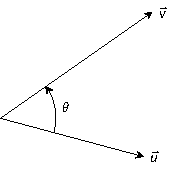
\includegraphics{figures/figdotpangle}\\
(a)\\[15pt]
\myincludegraphicsthree{width=125pt,3Dmenu,activate=onclick,deactivate=onclick,
3Droll=0,
3Dortho=0.0045,
3Dc2c=.54 .61 .58,
3Dcoo=0 0 40,
3Droo=170,
3Dlights=Headlamp,add3Djscript=asylabels.js}{}{figures/figdotpangle3D}\\
%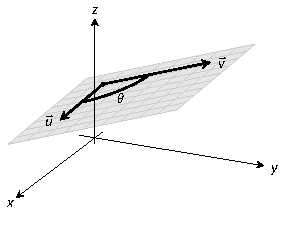
\includegraphics{figures/figdotpangle3D}\\
(b)
\end{tabular}
}

The same is also true of 2 vectors in space: given $\vec u$ and $\vec v$ in $\mathbb{R}^3$ with the same initial point, there is a plane that contains both $\vec u$ and $\vec v$. (When $\vec u$ and $\vec v$ are co-linear, there are infinite planes that contain both vectors.) In that plane, we can again find an angle $\theta$ between them (and again, $0\leq \theta\leq \pi$). This is illustrated in Figure \ref{fig:dotpangle}(b).

The following theorem connects this angle $\theta$ to the dot product of $\vec u$ and $\vec v$.

\theorem{thm:dot_product}{The Dot Product and Angles}
{Let $\vec u$ and $\vec v$ be vectors in $\mathbb{R}^2$ or $\mathbb{R}^3$. Then 
\[
\dotp uv = \norm{\vec u}\,\norm{\vec v} \cos\theta,
\]
where $\theta$, $0\leq\theta\leq \pi$, is the angle between $\vec u$ and $\vec v$.
\index{dot product!properties}\index{vectors!dot product}
}

\mfigure{.16}{Proving Theorem \ref{thm:dot_product}}{fig:dotprodproof}{figures/dotproductproof}

The proof of Theorem \ref{thm:dot_product} is an application of the \href{https://en.wikipedia.org/wiki/Law_of_cosines}{\underline{Law of Cosines}}, using the properties in Theorem \ref{thm:dot_product_properties}. Referring to Figure \ref{fig:dotprodproof}, if we let $a=\len{\vec u}$, $b=\len{\vec v}$, and $c = \len{\vec u-\vec v}$, then the Law of Cosines tells us that
\[
c^2 = a^2+b^2 - 2ab\cos(\theta).
\]
Thus, we have
\begin{align*}
\len{\vec{u}-\vec{v}}^2 & = \len{\vec{u}}^2+\len{\vec{v}}^2-2\len{\vec{u}}\len{\vec{v}}\cos\theta\\
(\vec u-\vec v)\boldsymbol{\cdot}(\vec u-\vec v) & = \dotp uu +\dotp vv -2\len{\vec{u}}\len{\vec{v}}\cos\theta\\
\dotp uu -\dotp uv - \dotp vu + \dotp vv & = \dotp uu +\dotp vv -2\len{\vec{u}}\len{\vec{v}}\cos\theta\\
-2\dotp uv &= -2\len{\vec{u}}\len{\vec{v}}\cos\theta\\
\dotp uv &= \len{\vec{u}}\len{\vec{v}}\cos\theta,
\end{align*}
as required.

When $\theta$ is an acute angle (i.e., $0\leq \theta <\pi/2$), $\cos \theta$ is positive; when $\theta = \pi/2$, $\cos \theta = 0$; when $\theta$ is an obtuse angle ($\pi/2<\theta \leq \pi$), $\cos \theta$ is negative. Thus the sign of the dot product gives a general indication of the angle between the vectors, illustrated in Figure \ref{fig:dotpsign}.

\begin{center}
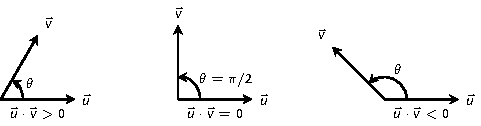
\includegraphics{figures/figdotpanglesign}
\captionsetup{type=figure}
\caption{Illustrating the relationship between the angle between vectors and the sign of their dot product.}
\label{fig:dotpsign}
\end{center}
\vskip\baselineskip

We \emph{can} use Theorem \ref{thm:dot_product} to compute the dot product, but generally this theorem is used to find the angle between known vectors (since the dot product is generally easy to compute). To this end, we rewrite the theorem's equation as
\[
\cos \theta = \frac{\dotp uv}{\norm{\vec u}\norm{\vec v}} \quad \Leftrightarrow \quad \theta = \cos^{-1}\left(\frac{\dotp uv}{\norm{\vec u}\norm{\vec v}}\right).
\]

We practice using this theorem in the following example.\\

\mfigure{.4}{Vectors used in Example \ref{ex_dotp2}.}{fig:dotp2}{figures/figdotp2}
\example{ex_dotp2}{Using the dot product to find angles}{
Let $\vec u = \la 3,1\ra$, $\vec v = \la -2,6\ra$ and $\vec w = \la -4,3\ra$, as shown in Figure \ref{fig:dotp2}. Find the angles $\alpha$, $\beta$ and $\theta$.
}
{We start by computing the magnitude of each vector.
\[
\norm{\vec u} = \sqrt{10};\quad \norm{\vec v} = 2\sqrt{10};\quad \norm{\vec w} = 5.
\]
We now apply Theorem \ref{thm:dot_product} to find the angles.
\begin{align*}
\alpha &= \cos^{-1}\left(\frac{\dotp uv}{(\sqrt{10})(2\sqrt{10})}\right) \\
			&= \cos^{-1}(0) = \frac{\pi}2 = 90^\circ.
\end{align*}
\begin{align*}
\beta &= \cos^{-1}\left(\frac{\dotp vw}{(2\sqrt{10})(5)}\right) \\
			&= \cos^{-1}\left(\frac{26}{10\sqrt{10}}\right) \\
					&\approx 0.6055 \approx 34.7^\circ.\\[10pt]
\theta &= \cos^{-1}\left(\frac{\dotp uw}{(\sqrt{10})(5)}\right) \\
				&= \cos^{-1}\left(\frac{-9}{5\sqrt{10}}\right) \\
				&\approx 2.1763 \approx 124.7^\circ
\end{align*}
\vskip-\baselineskip
}\\

We see from our computation that $\alpha + \beta = \theta$, as indicated by Figure \ref{fig:dotp2}. While we knew this should be the case, it is nice to see that this non-intuitive formula indeed returns the results we expected.

We do a similar example next in the context of vectors in space.\\

\example{ex_dotp3}{Using the dot product to find angles}{
Let $\vec u = \la 1,1,1\ra$, $\vec v = \la -1,3,-2\ra$ and $\vec w = \la -5,1,4\ra$, as illustrated in Figure \ref{fig:dotp3}. Find the angle between each pair of vectors.}
{\begin{enumerate}
	\item Between $\vec u$ and $\vec v$:
	\begin{align*}
	\theta &= \cos^{-1}\left(\frac{\dotp uv}{\norm{\vec u}\norm{\vec v}}\right)\\
					&= \cos^{-1}\left(\frac{0}{\sqrt{3}\sqrt{14}}\right)\\
					&= \frac{\pi}2.
	\end{align*}
	\item	Between $\vec u$ and $\vec w$:
	\begin{align*}
	\theta &= \cos^{-1}\left(\frac{\dotp uw}{\norm{\vec u}\norm{\vec w}}\right)\\
					&= \cos^{-1}\left(\frac{0}{\sqrt{3}\sqrt{42}}\right)\\
					&= \frac{\pi}2.
	\end{align*}
	\item	Between $\vec v$ and $\vec w$:
	\begin{align*}
	\theta &= \cos^{-1}\left(\frac{\dotp vw}{\norm{\vec v}\norm{\vec w}}\right)\\
					&= \cos^{-1}\left(\frac{0}{\sqrt{14}\sqrt{42}}\right)\\
					&= \frac{\pi}2.
	\end{align*}
\end{enumerate}
While our work shows that each angle is $\pi/2$, i.e.,  $90^\circ$, none of these angles looks to be a right angle in Figure \ref{fig:dotp3}. Such is the case when drawing three--dimensional objects on the page.
}\\

\mfigurethree{width=150pt,3Dmenu,activate=onclick,deactivate=onclick,
3Droll=0,
3Dortho=0.0045,
3Dc2c=.89 .4 .23,
3Dcoo=10 50 46,
3Droo=200,
3Dlights=Headlamp,add3Djscript=asylabels.js}{}{.7}{Vectors used in Example \ref{ex_dotp3}.}{fig:dotp3}{figures/figdotp3}%

All three angles between these vectors was $\pi/2$, or $90^\circ$. We know from geometry and everyday life that $90^\circ$ angles are ``nice'' for a variety of reasons, so it should seem significant that these angles are all $\pi/2$. Notice the common feature in each calculation (and also the calculation of $\alpha$ in Example \ref{ex_dotp2}): the dot products of each pair of angles was 0. We use this as a basis for a definition of the term \textbf{orthogonal}, which is essentially synonymous to \textit{perpendicular}.

\definition{def:orthogonal}{Orthogonal}
{Vectors $\vec u$ and $\vec v$ are \textbf{orthogonal} if their dot product is 0.
\index{orthogonal}\index{perpendicular|see{orthogonal}}\index{vectors!orthogonal}
}

\mnote{.22}{\textbf{Note:} The term \textit{perpendicular} originally referred to lines. As mathematics progressed, the concept of ``being at right angles to'' was applied to other objects, such as vectors and planes, and the term \emph{orthogonal} was introduced. It is especially used when discussing objects that are hard, or impossible, to visualize: two vectors in 5-dimensional space are orthogonal if their dot product is 0. It is not wrong to say they are \textit{perpendicular}, but common convention gives preference to the word \textit{orthogonal}.

Note also that Definition \ref{def:orthogonal} makes sense if either $\vec u$ or $\vec v$ is the zero vector, but this is not the case for the conventional understanding of the word perpendicular.
}

\pagebreak

\example{ex_dotp8}{Finding orthogonal vectors}{
Let $\vec u = \la 3,5\ra$ and $\vec v = \la 1,2,3\ra$. 
\begin{enumerate}
	\item Find two vectors in $\mathbb{R}^2$ that are orthogonal to $\vec u$.
	\item	Find two non--parallel vectors in $\mathbb{R}^3$ that are orthogonal to $\vec v$.
\end{enumerate}
}
{\begin{enumerate}
	\item Recall that a line perpendicular to a line with slope $m$ has slope $-1/m$, the ``opposite reciprocal slope.'' We can think of the slope of $\vec u$ as $5/3$, its ``rise over run.'' A vector orthogonal to $\vec u$ will have slope $-3/5$. There are many such choices, though all parallel:
	\[
	\la -5,3\ra \quad \text{or} \quad\la 5,-3\ra \quad \text{or} \quad \la -10,6\ra\quad \text{or} \quad \la 15,-9\ra,\text{etc.}
	\]
	\item		There are infinite directions in space orthogonal to any given direction, so there are an infinite number of non--parallel vectors orthogonal to $\vec v$. Since there are so many, we have great leeway in finding some.
	
	One way is to arbitrarily pick values for the first two components, leaving the third unknown. For instance, let $\vec v_1 = \la 2,7,z\ra$. If $\vec v_1$ is to be orthogonal to $\vec v$, then $\vec v_1\cdot\vec v = 0$, so 
	\[
	2+14+3z=0 \quad \Rightarrow z = \frac{-16}{3}.
	\]
	So $\vec v_1 = \la 2, 7, -16/3\ra$ is orthogonal to $\vec v$. We can apply a similar technique by leaving the first or second component unknown.
	
	Another method of finding a vector orthogonal to $\vec v$ mirrors what we did in part 1. Let $\vec v_2 = \la-2,1,0\ra$. Here we switched the first two components of $\vec v$, changing the sign of one of them (similar to the ``opposite reciprocal'' concept before). Letting the third component be 0 effectively ignores the third component of $\vec v$, and it is easy to see that 
	\[
	\vec v_2\cdot\vec v = \la -2,1,0\ra\cdot\la 1,2,3\ra = 0.
	\]
	Clearly $\vec v_1$ and $\vec v_2$ are not parallel.
\end{enumerate}
\vskip-1.5\baselineskip
}\\

An important construction is illustrated in Figure \ref{fig:dotpproj}, where vectors $\vec u$ and $\vec v$ are sketched. In part (a), a dotted line is drawn from the tip of $\vec u$ to the line containing $\vec v$, where the dotted line is orthogonal to $\vec v$. In part (b), the dotted line is replaced with the vector $\vec z$ and  $\vec w$ is formed, parallel to $\vec v$. It is clear by the diagram that $\vec u = \vec w+\vec z$. What is important about this construction is this: $\vec u$ is \emph{decomposed} as the sum of two vectors, one of which is parallel to $\vec v$ and one that is perpendicular to $\vec v$. It is hard to overstate the importance of this construction (as we'll see in upcoming examples). 

The vectors $\vec w$, $\vec z$ and $\vec u$ as shown in Figure \ref{fig:dotpproj} (b) form a right triangle, where the angle between $\vec v$ and $\vec u$ is labeled $\theta$. We can find $\vec w$ in terms of $\vec v$ and $\vec u$.

Using trigonometry, we can state that 
\begin{equation}
\norm{\vec w} = \norm{\vec u}\cos \theta. \label{eq:proj1}
\end{equation}
\mtable{.24}{Developing the construction of the \emph{orthogonal projection}.}{fig:dotpproj}{%
\begin{tabular}{c}
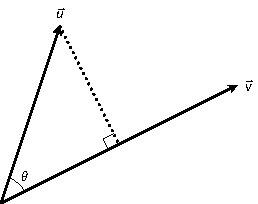
\includegraphics{figures/figdotpproja}\\
(a)\\[15pt]
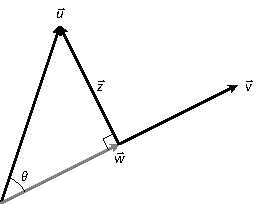
\includegraphics{figures/figdotpprojb}\\
(b)
\end{tabular}
}

We also know that $\vec w$ is parallel to to $\vec v$\,; that is, the direction of $\vec w$ is the direction of $\vec v$, described by the unit vector $\frac{1}{\norm{\vec v}}\vec v$. The vector $\vec w$ is the vector in the direction $\frac{1}{\norm{\vec v}}\vec v$ with magnitude $\norm{\vec u}\cos \theta$:

\begin{align*}
\vec w &= \Big(\norm{\vec u}\cos\theta \Big)\frac{1}{\norm{\vec v}}\vec v.\\
&= \left(\norm{\vec u}\frac{\dotp uv}{\norm{\vec u}\norm{\vec v}}\right)\frac{1}{\norm{\vec v}} \vec v \tag*{Replace $\cos\theta$ using Theorem \ref{thm:dot_product}}\\ 
			&= \frac{\dotp uv}{\norm{\vec v}^2}\vec v = \frac{\dotp uv}{\dotp vv}\vec v \tag*{Using Theorem \ref{thm:dot_product_properties}.}
\end{align*}

Since this construction is so important, it is given a special name.

\definition{def:orthogonal_projection}{Orthogonal Projection}
{Let $\vec u$ and $\vec v$ be given. The \textbf{orthogonal projection of $\vec u$ onto $\vec v$}, denoted $\proj uv$, is 
\index{orthogonal projection}\index{vectors!orthogonal projection}
\[
\proj uv = \left(\frac{\dotp uv}{\dotp vv}\right)\vec v.
\]
}\\

\enlargethispage{2\baselineskip}

\example{ex_dotp4}{Computing the orthogonal projection}{
\begin{enumerate}
	\item Let $\vec u= \la -2,1\ra$ and $\vec v=\la 3,1\ra$. Find $\proj uv$, and sketch all three vectors with initial points at the origin.
	\item	Let $\vec w = \la 2,1,3\ra$ and $\vec x = \la 1,1,1\ra$. Find $\proj wx$, and sketch all three vectors with initial points at the origin.
\end{enumerate}
}
{\begin{enumerate}
	\item Applying Definition \ref{def:orthogonal_projection}, we have
	\begin{align*}
	\proj uv &= \left(\frac{\dotp uv}{\dotp vv}\right)\vec v \\
					&= \frac{-5}{10}\la 3,1\ra\\
					&= \la -\frac32,-\frac12\ra.
	\end{align*}
	Vectors $\vec u$, $\vec v$ and $\proj uv$ are sketched in Figure \ref{fig:dotp4}(a). Note how the projection is parallel to $\vec v$; that is, it lies on the same line through the origin as $\vec v$, although it points in the opposite direction. That is because the angle between $\vec u$ and $\vec v$ is obtuse (i.e., greater than $90^\circ$).
\mtable{.37}{Graphing the vectors used in Example \ref{ex_dotp4}.}{fig:dotp4}{%
\begin{tabular}{c}
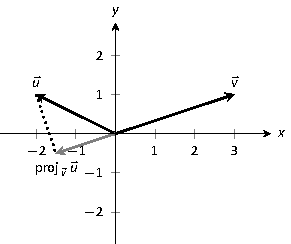
\includegraphics{figures/figdotp4a}\\
(a)\\[15pt]
\myincludegraphicsthree{width=100pt,3Dmenu,activate=onclick,deactivate=onclick,
3Droll=0,
3Dortho=0.0046,
3Dc2c=.9 .12 .42,
3Dcoo=0 50 30,
3Droo=250,
3Dlights=Headlamp,add3Djscript=asylabels.js}{}{figures/figdotp4b}\\
%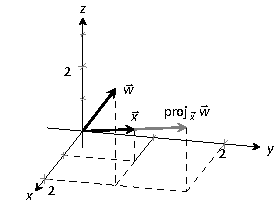
\includegraphics{figures/figdotp4b}\\
(b)\\[15pt]
\myincludegraphicsthree{width=100pt,3Dmenu,activate=onclick,deactivate=onclick,
3Droll=0,
3Dortho=0.0046,
3Dc2c=.29 .77 .56,
3Dcoo=50 0 40,
3Droo=250,
3Dlights=Headlamp,add3Djscript=asylabels.js}{}{figures/figdotp4c}\\
%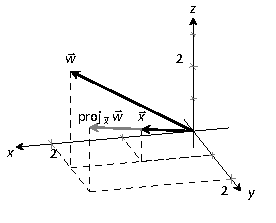
\includegraphics{figures/figdotp4c}\\
(c)\\[15pt]
\end{tabular}
}	
	
	\item		Apply the definition:
	\begin{align*}
	\proj wx &= \frac{\dotp wx}{\dotp xx}\vec x \\
					&= \frac{6}{3}\la 1,1,1\ra\\
					&= \la 2,2,2\ra.
	\end{align*}
	These vectors are sketched in Figure \ref{fig:dotp4}(b), and again in part (c) from a different perspective. Because of the nature of graphing these vectors, the sketch in part (b) makes it difficult  to recognize that the drawn projection has the geometric properties it should. The graph shown in part (c) illustrates these properties better.
\end{enumerate}
\vskip-\baselineskip
}

\pagebreak

Consider Figure \ref{fig:dotpprojc} where the concept of the orthogonal projection is again illustrated. It is clear that 
\begin{equation}
\vec u = \proj uv + \vec z.
\label{eq:orthogproj}
\end{equation} As we know what $\vec u$ and $\proj uv$ are, we can solve for $\vec z$ and state that
\[
\vec z = \vec u - \proj uv.
\]
This leads us to rewrite Equation \eqref{eq:orthogproj} in a seemingly silly way: 
\[
\vec u = \proj uv + (\vec u - \proj uv).
\]
This is not nonsense, as pointed out in the following Key Idea. (Notation note: the expression ``$\parallel \vec y$\,'' means ``is parallel to $\vec y$.'' We can use this notation to state ``$\vec x\parallel\vec y$\,'' which means ``$\vec x$ is parallel to $\vec y$.'' The expression ``$\perp \vec y$\,'' means ``is orthogonal to $\vec y$,'' and is used similarly.)

\mfigure{.73}{Illustrating the orthogonal projection.}{fig:dotpprojc}{figures/figdotpprojc}

\mnote{.4}{\textbf{Note:} The argument leading to Definition \ref{def:orthogonal_projection} is not quite a proof, since it depended on choices made in forming the diagram in Figure \ref{fig:dotpproj}. However, we can easily verify that the result in Key Idea \ref{idea:orthog_proj} is always valid: since
\begin{align*}
\vec v\boldsymbol{\cdot}(\vec u - \proj uv) & = \dotp vu - \vec v\boldsymbol{\cdot}\left(\frac{\dotp uv}{\len{\vec{v}}^2}\vec{v}\right)\\
& = \dotp vu -\frac{\dotp uv}{\dotp vv}(\dotp vv)\\
& = \dotp vu - \dotp uv = 0
\end{align*}
for \textbf{any} vectors $\vec u$ and $\vec v\neq \vec 0$, we are guaranteed that the vector $u-\proj uv$ will always be orthogonal to $\vec v$.}

\keyidea{idea:orthog_proj}{Orthogonal Decomposition of Vectors}
{Let $\vec u$ and $\vec v$ be given. Then $\vec u$ can be written as the sum of two vectors, one of which is parallel to $\vec v$, and one of which is orthogonal to $\vec v$:
\index{orthogonal decomposition of vectors}\index{orthogonal!decomposition}\index{vectors!orthogonal decomposition}
\[
\vec u = \underbrace{\proj uv}_{\parallel\ \vec v}\ +\  (\underbrace{\vec u-\proj uv}_{\perp\ \vec v}).
\]
}

We illustrate the use of this equality in the following example.\\

\example{ex_dotp5}{Orthogonal decomposition of vectors}{
\begin{enumerate}
	\item Let $\vec u = \la -2,1\ra $ and $\vec v = \la 3,1\ra$ as in Example \ref{ex_dotp4}. Decompose $\vec u$ as the sum of a vector parallel to $\vec v$ and a vector orthogonal to $\vec v$.
	\item	Let $\vec w =\la 2,1,3\ra$ and $\vec x  =\la 1,1,1\ra$ as in Example \ref{ex_dotp4}. Decompose $\vec w$ as the sum of a vector parallel to $\vec x$ and a vector orthogonal to $\vec x$.
\end{enumerate}
}
{\begin{enumerate}
	\item In Example \ref{ex_dotp4}, we found that $\proj uv = \la -1.5,-0.5\ra$. Let 
	\[
	\vec z = \vec u - \proj uv = \la -2,1\ra - \la -1.5,-0.5\ra = \la-0.5, 1.5\ra.
	\]
	Is $\vec z$ orthogonal to $\vec v$\,? (I.e, is $\vec z \perp\vec v$\ ?) We check for orthogonality with the dot product:
	\[
	\dotp zv = \la -0.5,1.5\ra \cdot \la 3,1\ra =0.
	\]
	Since the dot product is 0, we know $\vec z \perp \vec v$. Thus:
	\begin{align*}
	\vec u &= \proj uv\ +\ (\vec u - \proj uv) \\
	\la -2,1\ra &= \underbrace{\la -1.5,-0.5\ra}_{\parallel\ \vec v}\ +\ \underbrace{\la -0.5,1.5\ra}_{\perp \ \vec v}.
	\end{align*}
	
	\item	We found in Example \ref{ex_dotp4} that $\proj wx = \la 2,2,2\ra$. Applying the Key Idea, we have:
	\[
	\vec z = \vec w - \proj wx = \la 2,1,3\ra  - \la 2,2,2\ra = \la 0,-1,1\ra.
	\]
	We check to see if $\vec z \perp \vec x$:
\[
\dotp zx = \la 0,-1,1\ra \cdot \la 1,1,1\ra = 0.
\]
	Since the dot product is 0, we know the two vectors are orthogonal.
	We now write $\vec w$ as the sum of two vectors, one parallel and one orthogonal to $\vec x$:
	\begin{align*}
	\vec w &= \proj wx\ +\ (\vec w - \proj wx) \\
	\la 2,1,3\ra &= \underbrace{\la 2,2,2\ra}_{\parallel\ \vec x}\ +\ \underbrace{\la 0,-1,1\ra}_{\perp \ \vec x} 
	\end{align*}
\end{enumerate}
\vskip-\baselineskip
}\\

We give an example of where this decomposition is useful.\\

\example{ex_dotp6}{Orthogonally decomposing a force vector}{
Consider Figure \ref{fig:dotp6}(a), showing a box weighing 50lb on a ramp that rises 5ft over a span of 20ft. Find the components of force, and their magnitudes, acting on the box (as sketched in part (b) of the figure):
\mtable{.4}{Sketching the ramp and box in Example \ref{ex_dotp6}. Note: \textit{The vectors are not drawn to scale.}}{fig:dotp6}{%
\begin{tabular}{c}
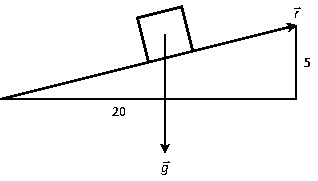
\includegraphics{figures/figdotp6}\\
(a)\\[15pt]
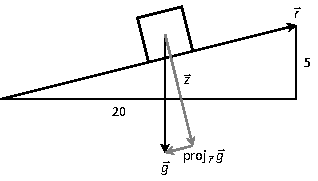
\includegraphics{figures/figdotp6b}\\
(b)
\end{tabular}
}
\begin{enumerate}
	\item in the direction of the ramp, and
	\item	orthogonal to the ramp.
\end{enumerate}
}
{As the ramp rises 5ft over a horizontal distance of 20ft, we can represent the direction of the ramp with the vector $\vec r= \la 20,5\ra$. Gravity pulls down with a force of 50lb, which we represent with $\vec g = \la 0,-50\ra$. 
\begin{enumerate}
	\item To find the force of gravity in the direction of the ramp, we compute $\proj gr$:
	\begin{align*}
	\proj gr &= \frac{\dotp gr}{\dotp rr}\vec r\\
					&=  \frac{-250}{425}\la 20,5\ra\\
					&= \la -\frac{200}{17},-\frac{50}{17}\ra \approx \la -11.76,-2.94\ra.
	\end{align*}
	The magnitude of $\proj gr$ is $\norm{\proj gr} = 50/\sqrt{17} \approx 12.13\text{lb}$. Though the box weighs 50lb, a force of about 12lb is enough to keep the box from sliding down the ramp.

\enlargethispage{2\baselineskip}
	
	\item		To find the component $\vec z$ of gravity orthogonal to the ramp, we use Key Idea \ref{idea:orthog_proj}.
	\begin{align*}
	\vec z &= \vec g - \proj gr \\
					&= \la \frac{200}{17},-\frac{800}{17}\ra \approx \la 11.76,-47.06\ra.
	\end{align*}
	The magnitude of this force is $\norm{\vec z} \approx 48.51$lb. In physics and engineering, knowing this force is important when computing things like static frictional force. (For instance, we could easily compute if the static frictional force alone was enough to keep the box from sliding down the ramp.)
\end{enumerate}
\vskip-\baselineskip
}

\pagebreak

\noindent\textbf{\large Application to Work}\\

In physics, the application of a force $F$ to move an object in a straight line a distance $d$ produces \emph{work}; the amount of work $W$ is $W=Fd$, (where $F$ is in the direction of travel). The orthogonal projection allows us to compute work when the force is not in the direction of travel.

Consider Figure \ref{fig:dotpwork}, where a force $\vec F$ is being applied to an object moving in the direction of $\vec d$. (The distance the object travels is the magnitude of $\vec d$.) The work done is the amount of force in the direction of $\vec d$, $\norm{\proj Fd}$, times $\vnorm d$:
\mfigure{.75}{Finding work when the force and direction of travel are given as vectors.}{fig:dotpwork}{figures/figdotpwork}

\begin{align*}
\norm{\proj Fd}\cdot\vnorm d &= \snorm{\frac{\dotp Fd}{\dotp dd}\vec d}\cdot \vnorm d \\
		&= \left|\frac{\dotp Fd}{\vnorm d^2}\right|\cdot \vnorm d\cdot\vnorm d\\
		&= \frac{\left|\dotp Fd\right|}{\vnorm d^2}\vnorm d^2\\
		&= \left|\dotp Fd\right|.
\end{align*}

The expression $\dotp Fd$ will be positive if the angle between $\vec F$ and $\vec d$ is acute; when the angle is obtuse (hence $\dotp Fd$ is negative), the force is causing motion in the opposite direction of $\vec d$, resulting in ``negative work.'' We want to capture this sign, so we drop the absolute value and find that $W = \dotp Fd$.

\definition{def:work}{Work}
{Let $\vec F$ be a constant force that moves an object in a straight line from point $P$ to point $Q$. Let $\vec d = \vv{PQ}$. The \textbf{work} $W$ done by $\vec F$ along $\vec d$ is $W = \dotp Fd$.
\index{work}
}

\example{ex_dotp7}{Computing work}{
A man slides a box along a ramp that rises 3ft over a distance of 15ft by applying 50lb of force as shown in Figure \ref{fig:dotp7}. Compute the work done.}
{The figure indicates that the force applied makes a $30^\circ$ angle with the horizontal, so $\vec F = 50\la \cos 30^\circ,\sin 30^\circ\ra \approx \la 43.3,25\ra.$ The ramp is represented by $\vec d  = \la 15,3\ra$. The work done is simply
\[
\dotp Fd = 50\la \cos 30^\circ,\sin 30^\circ\ra \cdot \la 15,3\ra \approx 724.5 \text{ft--lb}.
\]

\mfigure{.4}{Computing work when sliding a box up a ramp in Example \ref{ex_dotp7}.}{fig:dotp7}{figures/figdotp7}
Note how we did not actually compute the distance the object traveled, nor the magnitude of the force in the direction of travel; this is all inherently computed by the dot product!
}\\

The dot product is a powerful way of evaluating computations that depend on angles without actually using angles. The next section explores another ``product'' on vectors, the \emph{cross product.} Once again, angles play an important role, though in a much different way.

\printexercises{exercises/10_03_exercises}

\section{The Cross Product}\label{sec:cross_product}

``Orthogonality'' is immensely important. A quick scan of your current environment will undoubtedly reveal numerous surfaces and edges that are perpendicular to each other (including the edges of this page). The dot product provides a quick test for orthogonality:  vectors $\vec u$ and $\vec v$ are perpendicular if, and only if, $\dotp uv=0$. 

Given two non--parallel, nonzero vectors $\vec u$ and $\vec v$ in space, it is very useful to find a vector $\vec w$ that is perpendicular to both $\vec u$ and $\vec v$. There is a operation, called the \textbf{cross product}, that creates such a vector. This section defines the cross product, then explores its properties and applications.

\definition{def:cross_product}{Cross Product}
{Let $\vec u =\la u_1,u_2,u_3\ra$ and $\vec v = \la v_1,v_2,v_3\ra$ be vectors in $\mathbb{R}^3$. The \textbf{cross product of $\vec u$ and $\vec v$}, denoted $\crossp uv$, is the vector
\index{vectors!cross product}\index{cross product!definition}
\[
\crossp uv = \la u_2v_3-u_3v_2,u_3v_1-u_1v_3,u_1v_2-u_2v_1\ra.
\]
}

\mnote{.6}{The definition of the cross product may look strange (and complicated) at first, but it's more or less forced by the requirement that it be orthogonal to both $\vec u$ and $\vec v$. To begin to see why, suppose $\vec w = \la a,b,c\ra$ is an arbitrary vector such that $\dotp wu=0$ and $\dotp wv=0$. This gives us the pair of equations
\begin{align*}
u_1a+u_2b+u_3c&=0\\
v_1a+v_2b+v_3c&=0.
\end{align*}
This is a \textit{system of linear equations} in the variables $a$, $b$, and $c$. We'll learn the techniques for solving any such system in Chapter \ref{chapter:linear}, at which point we'll be able to see that (up to a scalar multiple) the solution is given by Definition \ref{def:cross_product}.}

This definition can be a bit cumbersome to remember. After an example we will give a convenient method for computing the cross product. For now, careful examination of the products and differences given in the definition should reveal a pattern that is not too difficult to remember. (For instance, in the first component only 2 and 3 appear as subscripts; in the second component, only 1 and 3 appear as subscripts. Further study reveals the order in which they appear.)

Let's practice using this definition by computing a cross product.\\

\example{ex_crossp1}{Computing a cross product}{
Let $\vec u = \la 2,-1,4\ra$ and $\vec v = \la 3,2,5\ra$. Find $\crossp uv$, and verify that it is orthogonal to both $\vec u$ and $\vec v$.
}
{Using Definition \ref{def:cross_product}, we have
\begin{align*}
\crossp uv &= \la u_2v_3-u_3v_2,u_3v_1-u_1v_3,u_1v_2-u_2v_1\ra\\
		   &= \la (-1)5-(4)2,(4)3-(2)5, (2)2-(-1)3\ra = \la -13,2,7\ra.
\end{align*}
(We encourage the reader to compute this product on their own, then verify their result.)

We test whether or not $\crossp uv$ is orthogonal to $\vec u$ and $\vec v$ using the dot product:
\begin{align*}
\big(\crossp uv\big) \cdot \vec u &= \la -13,2,7\ra \cdot \la 2,-1,4\ra = 0,\\
\big(\crossp uv\big) \cdot \vec v &= \la -13,2,7\ra \cdot \la 3,2,5 \ra = 0.
\end{align*}
Since both dot products are zero, $\crossp uv$ is indeed orthogonal to both $\vec u$ and $\vec v$.
}\\

We now introduce a method for computing the cross-product that is easier to remember, and has the added benefit of allowing us to preview \sword{determinants}, which we will return to in earnest in Section \ref{sec:determinant_1}. 

Consider a rectangular array $\bbm a&b\\c&d\ebm$ of four real numbers $a,b,c$, and $d$. A $2\times 2$ determinant takes any such array and assigns the number $ad-bc$. This is commonly denoted as follows:
\[
\bvm a&b\\c&d\evm = ad-bc.
\]
Most people find it easiest to remember this in terms of the two \textit{diagonals} of the array: we take the product of the two numbers on the \textit{main diagonal} (top-left to bottom-right), and subtract the product of the two numbers on the other diagonal:
\btz [baseline=-3pt,>=stealth]
\node at (0,0) {$\bvm a & b\\ c& d\evm$};
\draw[->,  thin] (-.5,.4) -- (.6,-.6) node[below right] {$ac\vphantom{bd}$};
\draw[->, thin] (0.4,.4) -- (-.6,-.6) node[below left ] {$bd$};
\etz

For example, we have $\bvm 4&-2\\6&3\evm = 4(3)-(-2)(6)=24$. Once we get comfortable with $2\times 2$ determinants, we can write the cross product in terms of them, as follows:
\begin{align}
\crossp uv &= \bvm u_2&u_3\\v_2&v_3\evm \veci - \bvm u_1&u_3\\v_1&v_3\evm\vecj + \bvm u_1&u_2\\v_1&v_2\evm\veck\label{eq:crossdet}\\ 
& = (u_2v_3-u_3v_2)\veci-(u_3v_1-u_1v_3)\vecj + (u_1v_2-u_2v_1)\veck,\nonumber
\end{align}
as before. Now, this might not seem like much of an improvement over the previous formula, so we take things one step further. First, we form a $3\times 3$ array as shown below. 
\[
\bvm \veci&\vecj&\veck\\u_1&u_2&u_3\\v_1&v_2&v_3\evm.
\]
The first row comprises the standard unit vectors $\vec i$, $\vec j$, and $\vec k$. The second and third rows are the vectors $\vec u$ and $\vec v$, respectively. Next, we \textit{expand} our $3\times 3$ array as a vector, where the coefficient of each standard unit vector is given by the $2\times 2$ determinant that's left over when we delete the row and column containing that unit vector. 

For example, if we use $\vec u$ and $\vec v$ from Example \ref{ex_crossp1}, we obtain the array
\[
\bvm \veci&\vecj&\veck \\  2&-1&4\\3&2&5\evm.
\]
The expansion process used to obtain the coefficients of $\veci, \vecj \veck$ looks like the following:

\btz [baseline=-3pt,>=stealth]
\node at (0,0) {$\bvm \fbox{\veci}&\vecj&\veck \\  2&-1&4\\3&2&5\evm\longrightarrow \bvm -1&4\\2&5\evm\veci = -13\veci$};
\draw[thin] (-2.3,.6) -- (-2.3, -.6);
\draw[thin] (-2.5,.4) -- (-.8,.4);
\etz

\btz [baseline=-3pt,>=stealth]
\node at (0,0) {$\bvm \veci&\fbox{\vecj}&\veck \\  2&-1&4\\3&2&5\evm\longrightarrow \bvm 2&4\\3&5\evm\vecj = -2\vecj$};
\draw[thin] (-1.45,.6) -- (-1.45, -.6);
\draw[thin] (-2.3,.4) -- (-.6,.4);
\etz

\btz [baseline=-3pt,>=stealth]
\node at (0,0) {$\bvm \veci&\vecj&\fbox{\veck} \\  2&-1&4\\3&2&5\evm\longrightarrow \bvm 2&-1\\3&2\evm\veck = 7\veck$};
\draw[thin] (-0.85,.6) -- (-0.85, -.6);
\draw[thin] (-2.3,.4) -- (-.6,.4);
\etz

There is one more important detail to note: notice in Equation \eqref{eq:crossdet} that there is a \textbf{minus sign} in front of the coefficient of the unit vector $\vecj$. We need to make sure that the signs in front of each $2\times 2$ determinant follow this $+,\,-,\,+$ pattern when we expand our array as a vector. For the vectors $\vec u$ and $\vec v$ in Example \ref{ex_crossp1}, we end up with the following:
\begin{align*}
\crossp uv & = \bvm \veci&\vecj&\veck \\  2&-1&4\\3&2&5\evm  = \bvm -1&4\\2&5\evm\veci - \bvm 2&4\\3&5\evm\vecj + \bvm 2&-1\\3&2\evm\veck\\
& = -13\veci - (-2)\vecj + 7\veck = \la -13, 2, 7\ra,
\end{align*}
as before. The method will become more clear with a bit of practice.\\

\mnote{.75}{\textbf{Note:} If the minus sign in front of the $\vecj$ coefficient seems out of place to you, it might help to imagine wrapping our $3\times 3$ array around a cylinder (like the label on a tin can). If we read from left to right, \textit{beginning in the $\vecj$ column}, then we should place the $\veck$ column first, followed by the $\veci$ column. For the vectors $\vec{u}$ and $\vec{v}$ in Example \ref{ex_crossp1}, this would result in the coefficient $\bvm 4&2\\5&2\evm = 2$ for the $\vecj$ component, which has the correct sign. However, since our habit is to read starting from the far left, we tend to write the $\veci$ column first, and then introduce the minus sign to compensate.}


\example{ex_crossp2}{Computing a cross product}{
Let $\vecu=\la 1,3,6\ra$ and $\vec v = \la -1,2,1\ra$. Compute both $\crossp uv$ and $\crossp vu$.}
{To compute $\crossp uv$, we form our $3\times 3$ array as prescribed above, and expand it into a vector:
\begin{align*}
\crossp uv &= \bvm \veci & \vecj & \veck\\ 1& 3& 6\\ -1& 2& 1\evm = \bvm 3& 6\\2 &1\evm \veci - \bvm 1 & 6\\ -1& 1\evm\vecj +\bvm 1& 3\\ -1 & 2\evm\veck\\
		& = (3(1)-6(2))\veci -(1(1)-6(-1))\vecj + (1(2)-3(-1))\veck\\
		& = -9\veci-7\vecj+5\veck = \la -9, -7, 5\ra.
\end{align*}
To compute $\crossp vu$, we switch the second and third rows of the above matrix, then expand as before:
\begin{align*}
\crossp vu & = \bvm \veci & \vecj& \veck\\ -1 & 2& 1\\ 1& 3& 6\evm = \bvm 2 &1\\3 &6\evm\veci - \bvm -1& 1\\ 1& 6\evm\vecj + \bvm -1& 2\\ 1 &3\evm\veck\\
		   & = (2(6)-1(3))\veci-((-1)(6)-1(1))\vecj + ((-1)(3)-2(1))\veck\\
		   & = 9\veci+7\vecj -5\veck = \la 9, 7, -5\ra = -\crossp uv.
\end{align*}
Note how with the rows being switched, the products that once appeared on the right now appear on the left, and vice--versa, so that the result is the opposite of $\crossp uv$. We leave it to the reader to verify that each of these vectors is orthogonal to $\vec u$ and $\vec v$.
}\\

\noindent\textbf{\large Properties of the Cross Product}\\

It is not coincidence that $\crossp vu = -(\crossp uv)$ in the preceding example; one can show using Definition \ref{def:cross_product} that this will always be the case. The following theorem states several useful properties of the cross product, each of which can be verified by referring to the definition.

\setboxwidth{15pt}
%\noindent\hskip-50pt\begin{minipage}{\linewidth}
\theorem{thm:cross_prod_prop}{Properties of the Cross Product}
{Let $\vecu$, $\vecv$ and $\vecw$ be vectors in $\mathbb{R}^3$ and let $c$ be a scalar. The following identities hold:
\index{vectors!cross product}\index{cross product!properties}
\begin{enumerate}
	\item \parbox{167pt}{$\crossp uv = -(\crossp vu)$} Anticommutative Property
	\item	\begin{enumerate}
		\item \parbox{145pt}{$(\vec u+\vec v)\times \vecw = \crossp uw+\crossp vw$} Distributive Properties
		\item	$\vec u \times (\vec v+\vec w) = \crossp uv+\crossp uw$
	\end{enumerate}
	\item		$c(\crossp uv) = (c\vecu) \times \vec v = \vecu \times (c\vecv)$
	\item		\begin{enumerate}
		\item \parbox{145pt}{$(\crossp uv)\cdot \vecu = 0$} Orthogonality Properties
		\item	$(\crossp uv)\cdot \vecv = 0$
	\end{enumerate}
	\item		$\crossp uu = \vec 0$
	\item		$\crossp u0 = \vec 0$
	\item		\parbox{167pt}{$\vecu \boldsymbol{\cdot} (\vecv\times\vecw) = (\crossp uv)\boldsymbol{\cdot} \vecw$} Scalar Triple Product
\end{enumerate}
}
%\end{minipage}
\restoreboxwidth

We introduced the cross product as a way to find a vector orthogonal to two given vectors, but we did not give a proof that the construction given in Definition \ref{def:cross_product} satisfies this property. Theorem \ref{thm:cross_prod_prop} asserts this property holds; we leave it as a problem in the Exercise section to verify this.

The algebraic properties of the cross product in Theorem \ref{thm:cross_prod_prop} also give us an additional method for computing the cross product in terms of the unit vectors $\veci, \vecj, \veck$. We know from Property 5 that
\[
\veci\times\veci = \vec 0, \vecj\times\vecj = \vec 0, \veck\times\veck = \vec 0,
\]
and it's easy to check that
\[
\veci\times\vecj = \veck, \vecj\times\veck = \veci, \veck\times\veci=\vecj,
\]
and then Property 1 guarantees that
\[
\vecj\times \veci = -\veck, \veck\times\vecj = -\veci, \veci\times\veck = -\vecj.
\]
Using Properties 2 and 3, we can then compute, for example,
\begin{align*}
\la 2,0,3\ra\times \la -1,4,2\ra & = (2\veci +3\veck)\times (-\veci +4\vecj +2\veck)\\
& = -2(\veci \times \veci)+8(\veci \times\vecj)+4(\veci \times\veck)\\
& \quad \quad-3(\veck\times\veci)+12(\veck\times\vecj)+6(\veck\times\veck)\\
& = \vec 0+8\veck -4\vecj -3\vecj -12\veci + \vec 0 = \la -12, -7, 8\ra.
\end{align*}

Property 5 from the theorem is also left to the reader to prove in the Exercise section, but it reveals something more interesting than ``the cross product of a vector with itself is $\vec 0$.'' Let $\vec u$ and $\vec v$ be parallel vectors; that is, let there be a scalar $c$ such that $\vecv = c\vecu$. Consider their cross product:
\begin{align*}
\crossp uv &= \vecu \times (c\vec u) \\
					&=	\parbox{50pt}{$c(\crossp uu)$}\text{(by Property 3 of Theorem \ref{thm:cross_prod_prop})}\\
					&= \parbox{50pt}{$\vec 0$.}\text{(by Property 5 of Theorem \ref{thm:cross_prod_prop})}
\end{align*}

We have just shown that the cross product of parallel vectors is $\vec 0$. This hints at something deeper. Theorem \ref{thm:dot_product} related the angle between two vectors and their dot product; there is a similar relationship relating the cross product of two vectors and the angle between them, given by the following theorem.

\theorem{thm:cross_product}{The Cross Product and Angles}
{Let $\vec u$ and $\vec v$ be vectors in $\mathbb{R}^3$. Then
\[
\norm{\crossp uv} = \vnorm u\, \vnorm v \sin\theta,
\]
where $\theta$, $0\leq \theta \leq \pi$, is the angle between $\vecu$ and $\vecv$.
\index{vectors!cross product}\index{cross product!properties}
}

\mnote{.52}{\textbf{Note:} Definition \ref{def:orthogonal} (through Theorem \ref{thm:dot_product}) defines $\vec u$ and $\vec v$ to be orthogonal if $\vec u\cdot\vec v=0$. We could use Theorem \ref{thm:cross_product} to define $\vec u$ and $\vec v$ are parallel if $\vec u\times \vec v = 0$. By such a definition, $\vec 0$ would be both orthogonal and parallel to every vector. Apparent paradoxes such as this are not uncommon in mathematics and can be very useful. (See also the first marginal note on page \pageref{note:parallel}.)\label{note:crossp}}
Note that this theorem makes a statement about the \emph{magnitude} of the cross product. When the angle between $\vecu$ and $\vecv$ is 0 or $\pi$ (i.e., the vectors are parallel), the magnitude of the cross product is 0. The only vector with a magnitude of 0 is $\vec 0$ (see Property \ref{thm:zero_norm} of Theorem \ref{thm:vector_properties}), hence the cross product of  parallel vectors is $\vec 0$.\\

We provide some anecdotal evidence of the truth of this theorem in the following example.\\

\example{ex_crossp3}{The cross product and angles}{
Let $\vec u = \la 1,3,6\ra$ and $\vec v = \la -1,2,1\ra$ as in Example \ref{ex_crossp2}. Verify Theorem \ref{thm:cross_product} by finding $\theta$, the angle between $\vecu$ and $\vecv$, and the magnitude of $\crossp uv$.}
{We use Theorem \ref{thm:dot_product} to find the angle between $\vecu$ and $\vecv$. 
\begin{align*}
\theta &= \cos^{-1}\left(\frac{\dotp uv}{\vnorm u\, \vnorm v}\right) \\
			&= \cos^{-1}\left(\frac{11}{\sqrt{46}\sqrt{6}}\right)\\
			&\approx 0.8471 = 48.54^\circ.
\end{align*}

Our work in Example \ref{ex_crossp2} showed that $\crossp uv = \la -9,-7,5\ra$, hence $\norm{\crossp uv} = \sqrt{155}.$ Is $\norm{\crossp uv} = \vnorm u\, \vnorm v\sin\theta$? Using numerical approximations, we find:
\begin{align*}
\norm{\crossp uv} &=\sqrt{155}  & \vnorm u\,\vnorm v \sin\theta & = \sqrt{46}\sqrt{6}\sin 0.8471\\
									&\approx 12.45. & &\approx 12.45.
\end{align*}
Numerically, they seem equal. Using a right triangle, one can show that 
\[
\sin\left(\cos^{-1}\left(\frac{11}{\sqrt{46}\sqrt{6}}\right)\right) = \frac{\sqrt{155}}{\sqrt{46}\sqrt{6}},
\]
which allows us to verify the theorem exactly.
}\\

To see that Theorem \ref{thm:cross_product} holds in general, let $\vec u=\la u_1,u_2,u_3\ra$ and $\vec v =\la v_1,v_2,v_3\ra$ be two arbitrary vectors in $\R^3$. Since the angle between $\vec u$ and $\vec v$ is defined to lie between 0 and $\pi$, we know that $\sin\theta\geq 0$, so that both sides of the equation $\len{\crossp uv} = \len{\vec{u}}\len{\vec v}\sin\theta$ are positive. Thus, we can show that both sides are equal if we can show that their squares are equal. We have
\begin{align*}
(\len{\vec u}\len{\vec v}\sin\theta)^2 & = \len{\vec u}^2\len{\vec v}^2\sin^2\theta\\
& = \len{\vec u}^2\len{\vec v}^2(1-\cos^2\theta) \tag*{since $\sin^2\theta+\cos^2\theta=1$}\\
& = \len{\vec u}^2\len{\vec v}^2-(\len{\vec u}\len{\vec v}\cos\theta)^2\\
& = \len{\vec u}^2\len{\vec v}^2-(\dotp uv)^2 \tag*{by Theorem \ref{thm:dot_product}}\\
& = (u_1^2+u_2^2+u_3^2)(v_1^2+v_2^2+v_3^2)-(u_1v_1+u_2v_2+u_3v_3)^2\\
& = u_2^2v_3^2 - 2u_2u_3v_2v_3 + u_3^2v_2^2 + u_1v_3^2 - 2u_1u_3v_1v_3 \tag*{$+ u_3^2v_1^2 + u_1^2v_2^2 - 2u_1u_2v_1v_2 + u_2^2v_1^2$}\\
& = (u_2v_3-u_3v_2)^2+(u_3v_1-u_1v_3)^2+(u_1v_2-u_2v_2)^2\\
& = \len{\crossp uv}^2,
\end{align*}
as required.\\




\noindent\textbf{Right Hand Rule}\\

The anticommutative property of the cross product demonstrates that $\crossp uv$ and $\crossp vu$ differ only by a sign -- these vectors have the same magnitude but point in the opposite direction. When seeking a vector perpendicular to $\vec u$ and $\vec v$, we essentially have two directions to choose from, one in the direction of $\crossp uv$ and one in the direction of $\crossp vu$. Does it matter which we choose? How can we tell which one we will get without graphing, etc.?

Another wonderful property of the cross product, as defined, is that it follows the \textbf{right hand rule.} Given $\vec u$ and $\vec v$ in $\mathbb{R}^3$ with the same initial point, point the index finger of your right hand in the direction of $\vecu$ and let your middle finger point in the direction of $\vecv$ (much as we did when establishing the right hand rule for the 3-dimensional coordinate system). Your thumb will naturally extend in the direction of $\crossp uv$. One can ``practice'' this using Figure \ref{fig:crossp_rhr}. If you switch, and point the index finder in the direction of $\vecv$ and the middle finger in the direction of $\vecu$, your thumb will now point in the opposite direction, allowing you to ``visualize'' the anticommutative property of the cross product.
\mfigurethree{width=150pt,3Dmenu,activate=onclick,deactivate=onclick,
3Droll=0,
3Dortho=0.0044,
3Dc2c=.78 .32 .53,
3Dcoo=0 0 34,
3Droo=150,
3Dlights=Headlamp,add3Djscript=asylabels.js}{scale=1.25,trim=5mm 5mm 5mm 5mm,clip=true}{.5}{Illustrating the Right Hand Rule of the cross product.}{fig:crossp_rhr}{figures/figcrossp_rhr}
%\mfigure[scale=1.25,trim=5mm 5mm 5mm 5mm,clip=true]{.5}{Illustrating the Right Hand Rule of the cross product.}{fig:crossp_rhr}{figures/figcrossp_rhr}

\vskip\baselineskip
\noindent\textbf{\large Applications of the Cross Product}\\

There are a number of ways in which the cross product is useful in mathematics, physics and other areas of science beyond ``just'' finding a vector perpendicular to two others. We highlight a few here.\index{cross product!applications}\\
%\enlargethispage{\baselineskip}
%	\clearpage\enlargethispage{2\baselineskip}

\noindent\textbf{Area of a Parallelogram}\\

It is a standard geometry fact that the area of a parallelogram is $A = bh$, where $b$ is the length of the base and $h$ is the height of the parallelogram, as illustrated in Figure \ref{fig:crossp_parallelogram}(a). As shown when defining the Parallelogram Law of vector addition, two vectors $\vecu$ and $\vecv$ define a parallelogram when drawn from the same initial point, as illustrated in Figure \ref{fig:crossp_parallelogram}(b). Trigonometry tells us that $h = \vnorm u \sin \theta$, hence the area of the parallelogram is 
\begin{equation}A = \vnorm u\,\vnorm v\sin\theta = \norm{\crossp uv},\label{eq:crossp1}\end{equation}
where the second equality comes from Theorem \ref{thm:cross_product}.
\mtable{.23}{Using the cross product to find the area of a parallelogram.}{fig:crossp_parallelogram}{%
\begin{tabular}{c}
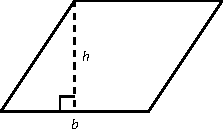
\includegraphics{figures/figcrossp_parallelogram1}\\
(a) \\[15pt]
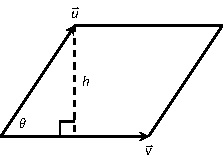
\includegraphics{figures/figcrossp_parallelogram2}\\
(b) \\
\end{tabular}
}
We illustrate using Equation \eqref{eq:crossp1} in the following example.
\index{cross product!applications!area of parallelogram}\\

\example{ex_crossp4}{Finding the area of a parallelogram}{
\begin{enumerate}
	\item Find the area of the parallelogram defined by the vectors $\vecu = \la 2,1\ra$ and $\vecv = \la 1,3\ra$.
	\item	Verify that the points $A = (1,1,1)$, $B = (2,3,2)$, $C = (4,5,3)$ and $D = (3,3,2)$ are the vertices of a parallelogram. Find the area of the parallelogram.
\end{enumerate}
}
{\begin{enumerate}
	\item Figure \ref{fig:crossp4}(a) sketches the parallelogram defined by the vectors $\vec u$ and $\vec v$. We have a slight problem in that our vectors exist in $\mathbb{R}^2$, not $\mathbb{R}^3$, and the cross product is only defined on vectors in $\mathbb{R}^3$. We skirt this issue by viewing $\vec u$ and $\vecv$ as vectors in the $x-y$ plane of $\mathbb{R}^3$, and rewrite them as $\vec u = \la 2,1,0\ra$ and $\vecv =\la 1,3,0\ra$. We can now compute the cross product. 
	It is easy to show that $\crossp uv = \la 0,0,5\ra$; therefore the area of the parallelogram is $A = \norm{\crossp uv} = 5$.
	\mtable{.65}{Sketching the parallelograms in Example \ref{ex_crossp4}.}{fig:crossp4}{%
	\begin{tabular}{c}
	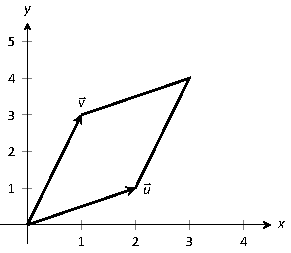
\includegraphics{figures/figcrossp4b}\\
	(a)\\[15pt]
	\myincludegraphicsthree{width=125pt,3Dmenu,activate=onclick,deactivate=onclick,
3Droll=0,
3Dortho=0.004,
3Dc2c=.42 .87 .26,
3Dcoo=61 60 63,
3Droo=250,
3Dlights=Headlamp,add3Djscript=asylabels.js}{scale=1.25,trim=4mm 5mm 4mm 5mm,clip=true}{figures/figcrossp4a}\\
	%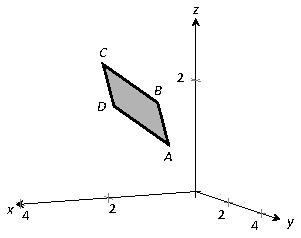
\includegraphics{figures/figcrossp4a}\\
	(b)
	\end{tabular}
	}
	\item		To show that the quadrilateral $ABCD$ is a parallelogram (shown in Figure \ref{fig:crossp4}(b)), we need to show that the opposite sides are parallel. We can quickly show that $\overrightarrow{AB} =\overrightarrow{DC} = \la 1,2,1\ra$ and $\overrightarrow{BC} = \overrightarrow{AD} = \la 2,2,1\ra$. We find the area by computing the magnitude of the cross product of $\overrightarrow{AB}$ and $\overrightarrow{BC}$:
\[
\overrightarrow{AB} \times \overrightarrow{BC} = \la 0,1,-2\ra \quad \Rightarrow \quad \norm{\overrightarrow{AB}\times\overrightarrow{BC}} = \sqrt{5} \approx 2.236.
\]
\end{enumerate}
\vskip-\baselineskip
}\\

This application is perhaps more useful in finding the area of a triangle (in short, triangles are used more often than parallelograms). We illustrate this in the following example.\\

\mfigure{.25}{Finding the area of a triangle in Example \ref{ex_crossp5}.}{fig:crossp5}{figures/figcrossp5}

\example{ex_crossp5}{Area of a triangle}{
Find the area of the triangle with vertices $A=(1,2)$, $B=(2,3)$ and $C=(3,1)$, as pictured in Figure \ref{fig:crossp5}.}
{We found the area of this triangle in Example \ref{ex_abc4} to be $1.5$ using integration. There we discussed the fact that finding the area of a triangle can be inconvenient using the ``$\frac12bh$'' formula as one has to compute the height, which generally involves finding angles, etc. Using a cross product is much more direct.

We can choose any two sides of the triangle to use to form vectors; we choose $\overrightarrow{AB} = \la 1,1\ra$ and $\overrightarrow{AC}=\la 2,-1\ra$. As in the previous example, we will rewrite these vectors with a third component of 0 so that we can apply the cross product. The area of the triangle is
\[
\frac12\norm{\overrightarrow{AB}\times\overrightarrow{AC}} = \frac12\norm{\la 1,1,0\ra \times \la 2,-1,0\ra} = \frac12\norm{\la 0,0,-3\ra} = \frac32.
\]
We arrive at the same answer as before with less work.
}\\



\pagebreak

\noindent\textbf{Volume of a Parallelepiped}

The three dimensional analogue to the parallelogram is the \textbf{parallelepiped}. Each face is parallel to the face opposite face, as illustrated in Figure \ref{fig:crossp_parallelepiped}. The volume of any three-dimensional solid whose cross-sectional area is a constant is given by $V=B\cdot h$, where $B$ is the area of the base (the constant cross-sectional area), and $h$ is the height. To determine a formula for the volume, we refer to Figure \ref{fig:parallelepiped_volume}. By crossing $\vec v$ and $\vec w$, one gets a vector whose magnitude is the area of the base, and whose direction is perpendicular to the parallelogram forming the base of the solid. We can then see that the height of the parallelepiped is equal to the length of the projection of the vector $\vec u$ onto $\crossp vw$. Thus, our volume is given by:
\begin{align*}
V & = B\cdot h\\
  & = \len{\crossp vw}\cdot \len{\operatorname{proj}_{\crossp vw}\vec{u}}\\
  & = \len{\crossp vw}\cdot\len{\left(\frac{\vec{u}\boldsymbol{\cdot}(\crossp vw)}{\len{\crossp vw}^2}\right)(\crossp vw)}\\
  & = \len{\crossp vw}\frac{\abs{\vec{u}\boldsymbol{\cdot}(\crossp vw)}}{\len{\crossp vw}^2}\len{\crossp vw}\\
  & = \abs{\vec{u}\boldsymbol{\cdot}(\crossp vw)}.
\end{align*}

\mfigurethree{width=75pt,3Dmenu,activate=onclick,deactivate=onclick,
3Droll=0,
3Dortho=0.0045,
3Dc2c=.84 .46 .26,
3Dcoo=0 110 86,
3Droo=150,
3Dlights=Headlamp,add3Djscript=asylabels.js}{}{.8}{A parallelepiped is the three dimensional analogue to the parallelogram.}{fig:crossp_parallelepiped}{figures/figcrosspparallelpiped}
%\mfigure{.53}{A parallelepiped is the three dimensional analogue to the parallelogram.}{fig:crossp_parallelepiped}{figures/figcrosspparallelpiped}
\index{cross product!applications!volume of parallelepiped}

Thus the volume of a parallelepiped defined by vectors $\vecu$, $\vecv$ and $\vec w$ is 
\begin{equation}
V = \abs{\vecu\boldsymbol{\cdot} (\crossp vw)}.\label{eq:crossp2}
\end{equation}
Note how this is the Scalar Triple Product, first seen in Theorem \ref{thm:cross_prod_prop}. Applying the identities given in the theorem shows that we can apply the Scalar Triple Product in any ``order'' we choose to find the volume. That is,
\[
V = |\vecu\boldsymbol{\cdot}(\crossp vw)| = |\vec u\boldsymbol{\cdot} (\crossp wv)| = |(\crossp uv)\boldsymbol{\cdot} \vecw|,\quad \text{etc.}
\]

\mfigure[width=0.95\marginparwidth]{.55}{Determining the volume of a parallelepiped}{fig:parallelepiped_volume}{figures/parallelepiped2}

\example{ex_crossp6}{Finding the volume of parallelepiped}{
Find the volume of the parallelepiped defined by the vectors $\vecu = \la 1,1,0\ra$, $\vecv = \la -1,1,0\ra$ and $\vecw = \la 0,1,1\ra$. 
}
{We apply Equation \eqref{eq:crossp2}. We first find $\crossp vw =\la 1,1,-1\ra$. Then
\[
|\vec u\cdot(\crossp vw)| = |\la 1,1,0\ra \cdot \la1,1,-1\ra| = 2.
\]
So the volume of the parallelepiped is 2 cubic units.
\mfigurethree{width=125pt,3Dmenu,activate=onclick,deactivate=onclick,
3Droll=0,
3Dortho=0.0045,
3Dc2c=4 4 2,
3Dcoo=0 50 50,
3Droo=150,
3Dlights=Headlamp,add3Djscript=asylabels.js}{}{.3}{A parallelepiped in Example \ref{ex_crossp6}.}{fig:crossp6}{figures/figcrossp6}
%\mfigure{.3}{A parallelepiped in Example \ref{ex_crossp6}.}{fig:crossp6}{figures/figcrossp6}
}\\

Let's take another look at how Equation \eqref{eq:crossp2} is computed in terms of our formulas for the dot and cross products. With $\vec u = \la u_1, u_2, u_3\ra, \vec v = \la v_1, v_2, v_3\ra$, and $\vec w = \la w_1, w_2, w_3\ra$, we have
\begin{align*}
\vec{u}\boldsymbol{\cdot}(\crossp vw) & = \la u_1, u_2, u_3\ra \boldsymbol{\cdot}\left\langle \bvm v_2 & v_3\\w_2&w_3\evm, -\bvm v_1 & v_3\\ w_1 & w_3\evm, \bvm v_1 & v_2\\ w_1 & w_2\evm\right\rangle\\
 & = u_1\bvm v_2 & v_3\\w_2&w_3\evm - u_2\bvm v_1 & v_3\\ w_1 & w_3\evm + u_3\bvm v_1 & v_2\\ w_1 & w_2\evm.
\end{align*}
Compare this with our determinant formula for computing the cross product,
\[
\crossp vw = \bvm \veci & \vecj & \veck\\ v_1 & v_2 & v_3\\ w_1 & w_2 & w_3\evm = \bvm v_2 & v_3\\w_2&w_3\evm\veci - \bvm v_1 & v_3\\ w_1 & w_3\evm\vecj + \bvm v_1 & v_2\\ w_1 & w_2\evm\veck.
\]
If we replace the unit vectors $\veci, \vecj, veck$ in the above equation with the components of $\vec{u}$, we arrive at our first instance of a \textbf{$3\times 3$ determinant}, along with a method for computing such an object:
\[
\bvm u_1 & u_2 & u_3\\ v_1 & v_2 & v_3\\ w_1 & w_2 & w_3\evm = u_1 \bvm v_2 & v_3\\ w_2 & w_3\evm - u_2\bvm v_1 & v_3\\ w_1 & w_3\evm + u_3\bvm v_1 & v_2\\ w_1 & w_2\evm = \vec u\boldsymbol{\cdot}(\crossp vw).
\]
We will return to our study of determinants in Section \ref{sec:determinant_1}, where we will learn techniques for efficiently computing determinants of any size.

While this application of the Scalar Triple Product is interesting, it is not used all that often: parallelepipeds are not a common shape in physics and engineering. (It is, however, essential to understanding the change of variables formula for multiple integrals in Calculus.) The last application of the cross product is very applicable in engineering.\\

\noindent\textbf{Torque}\\

\textbf{Torque} is a measure of the turning force applied to an object. A classic scenario involving torque is the application of a wrench to a bolt. When a force is applied to the wrench, the bolt turns. When we represent the force and wrench with vectors $\vec F$ and $\vec \ell$, we see that the bolt moves (because of the threads) in a  direction orthogonal to $\vec F$ and $\vec \ell$. Torque is usually represented by the Greek letter $\tau$, or tau, and has units of N$\cdot$m, a Newton--meter, or ft$\cdot$lb, a foot--pound.\index{cross product!applications!torque}

While a full understanding of torque is beyond the purposes of this book, when a force $\vec F$ is applied to a lever arm $\vec \ell$, the resulting torque is \begin{equation}\vec \tau = \crossp \ell F.\label{eq:crossp3}\end{equation}

\example{ex_crossp7}{Computing torque}{
A lever of length 2ft makes an angle with the horizontal of $45^\circ$. Find the resulting torque when a force of 10lb is applied to the end of the level where:
\begin{enumerate}
	\item the force is perpendicular to the lever, and
	\item	the force makes an angle of $60^\circ$ with the lever, as shown in Figure \ref{fig:crossp7}.
\end{enumerate}
}
{\begin{enumerate}
	\item We start by determining vectors for the force and lever arm. Since the lever arm makes a $45^\circ$ angle with the horizontal and is 2ft long, we can state that $\vec \ell = 2\la \cos 45^\circ,\sin 45^\circ\ra = \la \sqrt2,\sqrt2\ra.$
	
	Since the force vector is perpendicular to the lever arm (as seen in the left hand side of Figure \ref{fig:crossp7}), we can conclude it is making an angle of $-45^\circ$ with the horizontal. As it has a magnitude of 10lb, we can state $\vec F = 10\la \cos (-45^\circ), \sin(-45^\circ)\ra = \la 5\sqrt2,-5\sqrt2\ra.$
	
	Using Equation \eqref{eq:crossp3} to find the torque requires a cross product. We again let the third component of each vector be 0  and compute the cross product:
	\begin{align*}
	\vec\tau &= \crossp \ell F \\
				&= \la \sqrt2,\sqrt2,0\ra \times \la 5\sqrt2,-5\sqrt2,0\ra \\
				&= \la 0,0,-20\ra
	\end{align*}
	This clearly has a magnitude of 20 ft-lb.
	
	We can view the force and lever arm vectors as lying ``on the page''; our computation of $\vec\tau$ shows that the torque goes ``into the page.'' This follows the Right Hand Rule of the cross product, and it also matches well with the example of the wrench turning the bolt. Turning a bolt clockwise moves it in.
	
	\item		Our lever arm can still be represented by $\vec \ell = \la \sqrt2,\sqrt2\ra$. As our force vector makes a $60^\circ$ angle with $\vec \ell$, we can see (referencing the right hand side of the figure) that $\vec F$ makes a $-15^\circ$ angle with the horizontal. Thus 
	\begin{align*}
	\vec F = 10\la \cos-15^\circ,\sin-15^\circ\ra &= \la \frac{5(1+\sqrt3)}{\sqrt2},-\frac{5(1+\sqrt3)}{\sqrt2}\ra \\
	&\approx \la 9.659,-2.588\ra.\end{align*}
	
	We again make the third component 0 and take the cross product to find the torque:
	\begin{align*}
	\vec\tau &= \crossp \ell F\\
					&= \la \sqrt2,\sqrt2,0\ra \times  \la \frac{5(1+\sqrt3)}{\sqrt2},-\frac{5(1+\sqrt3)}{\sqrt2},0\ra\\
					&= \la 0,0,-10\sqrt3\ra\\
					&\approx \la 0,0,-17.321\ra.
	\end{align*}
	As one might expect, when the force and lever arm vectors \textit{are} orthogonal, the magnitude of force is greater than when the vectors \textit{are not} orthogonal.
\end{enumerate}
\vskip-\baselineskip
}\\

\mfigure{.6}{Showing a force being applied to a lever in Example \ref{ex_crossp7}.}{fig:crossp7}{figures/figcrossp7}

While the cross product has a variety of applications (as noted in this chapter), its fundamental use is finding a vector perpendicular to two others. Knowing a vector is orthogonal to two others is of incredible importance, as it allows us to find the equations of lines and planes in a variety of contexts. The importance of the cross product, in some sense, relies on the importance of lines and planes, which see widespread use throughout engineering, physics and mathematics. We study lines and planes in the next two sections. 

\printexercises{exercises/10_04_exercises}


\section{Lines}\label{sec:lines}

\index{lines}
To find the equation of a line in the $x$-$y$ plane, we need two pieces of information: a point and the slope. The slope conveys \textit{direction} information. As vertical lines have an undefined slope, the following statement is more accurate:

\begin{quotation}
\noindent To define a line, one needs a point on the line and the direction of the line.
\end{quotation}

This holds true for lines in space.\\

Let $P$ be a point in space, let $\vec p$ be the vector with initial point at the origin and terminal point at $P$ (i.e., $\vec p$ ``points'' to $P$), and let $\vec d$ be a vector. Consider the points on the line through $P$ in the direction of $\vec d$. 

Clearly one point on the line is $P$; we can say that the \emph{vector} $\vec p$ lies at this point on the line. To find another point on the line, we can start at $\vec p$ and move in a  direction parallel to $\vec d$. For instance, starting at $\vec p$ and traveling one length of $\vec d$ places one at another point on the line. Consider Figure \ref{fig:lines_intro} where certain points along the line are indicated. 
\mfigurethree{width=125pt,3Dmenu,activate=onclick,deactivate=onclick,
3Droll=0,
3Dortho=0.0045,
3Dc2c=.84 .46 .26,
3Dcoo=0 70 0,
3Droo=150,
3Dlights=Headlamp,add3Djscript=asylabels.js}{scale=1.25,trim=5mm 5mm 5mm 5mm,clip=true}{.7}{Defining a line in space.}{fig:lines_intro}{figures/figlines_intro}
%\mfigure[scale=1.25,trim=5mm 5mm 5mm 5mm,clip=true]{.7}{Defining a line in space.}{fig:lines_intro}{figures/figlines_intro}

The figure illustrates how every point on the line can be obtained by starting with $\vec p$ and moving a certain distance in the direction of $\vec d$. That is, we can define the line as a function of $t$:
\begin{equation}\vec\ell(t) = \vec p + t\ \vec d.\label{eq:lines1}\end{equation}

In many ways, this is \textit{not} a new concept. Compare Equation \eqref{eq:lines1} to the familiar ``$y=mx+b$'' equation of a line:

\begin{center}
\begin{tikzpicture}[>=stealth]
	\draw (0,0) node (L) {\large $y\ =\ b\ +\ m\,x$};
	\draw (5,0) node (R) {\large $\vec \ell(t)\ =\ \vec p\ +\ t\,\vec d$};
\node (A) at (1,1.5) [align=center,] {Starting\\ Point};
\node (B) at (4,1.5) [align=center] {Direction};
\node (C) at (2.5,-1.5) [align=center] {How Far To\\  Go In That \\Direction};
\draw [->,thick] (A) -- ($(R)+(-1pt,8pt)$);	
\draw [->,thick] (A) -- ($(L)+(-0pt,10pt)$);
\draw [->,thick] (B) -- (.9,.2);
\draw [->,thick] (B) -- ($(R)+(30pt,7pt)$);
\draw [->,thick] (C) -- (1.3,-.15);
\draw [->,thick] (C) -- ($(R)+(25pt,-7pt)$);
\end{tikzpicture}
\captionsetup{type=figure}%
\caption{Understanding the vector equation of a line.}
\label{fig:lines_eq}
\end{center}


%\begin{center}
%\begin{tikzpicture}[>=stealth]
	%\draw (0,0) node {\large $y\ =\ b\ +\ m\,x$};
%\node (A) at (-1,-1) [align=center,] {Starting\\ Point};
%\node (B) at (1,-1) [align=center] {Direction};
%\node (C) at (3,-1) [align=center] {How Far To\\  Go In That \\Direction};
%\draw [->,thick] (A) -- (-.3,-.2);	
%\draw [->,thick] (B) -- (.8,-.2);
%\draw [->,thick] (C) -- (1.3,-.15);
%\end{tikzpicture}
%\end{center}
%Now compare this to the formula given in Equation \eqref{eq:lines1}:
%\begin{center}
%\begin{tikzpicture}[>=stealth]
	%\draw (0,0) node {\large $\vec \ell(t)\ =\ \vec p\ +\ t\,\vec d$};
%\node (A) at (-1,-1) [align=center,] {Starting\\ Point};
%\node (B) at (.5,.75) [align=center] {Direction};
%\node (C) at (2,-1.25) [align=center] {How Far To\\  Go In That \\Direction};
%\draw [->,thick] (A) -- (-.05,-.2);	
%\draw [->,thick] (B) -- (1.2,.3);
%\draw [->,thick] (C) -- (1.0,-.2);
%\end{tikzpicture}
%\end{center}

The equations exhibit the same structure: they give a starting point, define a direction, and state how far in that direction to travel.

Equation \eqref{eq:lines1} is an example of a \textbf{vector--valued function}; the input of the function is a real number and the output is a vector. We will cover vector--valued functions extensively in the next chapter.

There are other ways to represent a line. Let $\vec p = \la x_0,y_0,z_0\ra$ and let $\vec d = \la a,b,c\ra$. Then the equation of the line through $\vec p$ in the direction of $\vec d$ is:
\begin{align*}
\vec\ell(t) &= \vec p + t\vec d \\
						&= \la x_0,y_0,z_0\ra + t\la a,b,c\ra \\
						&= \la x_0 + at, y_0+bt, z_0+ct\ra.
\end{align*}

The last line states the the $x$ values of the line are given by $x=x_0+at$, the $y$ values are given by $y = y_0+bt$, and the $z$ values are given by $z = z_0 + ct$. These three equations, taken together, are the \textbf{parametric equations of the line} through $\vec p$ in the direction of $\vec d$.

Finally, each of the equations for $x$, $y$ and $z$ above contain the variable $t$. We can solve for $t$ in each equation:
\begin{align*}
x = x_0+at \quad&\Rightarrow\quad t=\frac{x-x_0}{a},\\
y=y_0+bt \quad&\Rightarrow\quad t = \frac{y-y_0}{b},\\
z = z_0+ct \quad&\Rightarrow\quad t = \frac{z-z_0}{c},\\
\end{align*}
assuming $a,b,c\neq 0$.
Since $t$ is equal to each expression on the right, we can set these equal to each other, forming the \textbf{symmetric equations of the line} through $\vec p$ in the direction of $\vec d$:
\[
\frac{x-x_0}{a} = \frac{y-y_0}{b}=\frac{z-z_0}{c}.
\]
Each representation has its own advantages, depending on the context. We summarize these three forms in the following definition, then give examples of their use.
%\clearpage

\definition{def:lines}{Equations of Lines in Space}
{Consider the line in space that passes through $\vec p = \la x_0,y_0,z_0\ra$ in the direction of $\vec d = \la a,b,c\ra.$\index{lines!equations for}
\begin{enumerate}
	\item The \textbf{vector equation} of the line is 
	\[
	\vec \ell(t) = \vec p+t\vec d.
	\]
	\item	The \textbf{parametric equations} of the line are
	\[
	x = x_0+at, \quad y=y_0+bt, \quad z = z_0+ct .
	\]
	\item	The \textbf{symmetric equations} of the line are
	\[
	\frac{x-x_0}{a} = \frac{y-y_0}{b}=\frac{z-z_0}{c}.
	\]
\end{enumerate}
}

\example{ex_lines1}{Finding the equation of a line}{
Give all three equations, as given in Definition \ref{def:lines}, of the line through $P = (2,3,1)$ in the direction of $\vec d = \la -1,1,2\ra$. Does the point $Q=(-1,6,6)$ lie on this line?}
{We identify the point $P=(2,3,1)$ with the vector $\vec p =\la 2,3,1\ra$. Following the definition, we have
\begin{itemize}
	\item the vector equation of the line is $\vec\ell(t) = \la 2,3,1\ra + t\la -1,1,2\ra$;
	\item	the parametric equations of the line are
	\[
	x = 2-t,\quad y = 3+t,\quad z = 1+2t; \text{ and}
	\]
	\item	the symmetric equations of the line are
	\[
	\frac{x-2}{-1}=\frac{y-3}{1} = \frac{z-1}{2}.
	\]
\end{itemize}
\mfigurethree{width=125pt,3Dmenu,activate=onclick,deactivate=onclick,
3Droll=0,
3Dortho=0.0045,
3Dc2c=.78 .53 .32,
3Dcoo=0 70 50,
3Droo=150,
3Dlights=Headlamp,add3Djscript=asylabels.js}{scale=1.25,trim=2mm 2mm 2mm 2mm,clip=true}{.2}{Graphing a line in Example \ref{ex_lines1}.}{fig:lines1}{figures/figlines1}
%\mfigure[scale=1.25,trim=2mm 2mm 2mm 2mm,clip=true]{.5}{Graphing a line in Example \ref{ex_lines1}.}{fig:lines1}{figures/figlines1}

The first two equations of the line are useful when a $t$ value is given: one can immediately find the corresponding point on the line. These forms are good when calculating with a computer; most software programs easily handle equations in these formats. (For instance, to make Figure \ref{fig:lines1}, a certain graphics program was given the input \texttt{(2-x,3+x,1+2*x)}. This particular program requires the variable always be ``$x$'' instead of ``$t$'').

Does the point $Q = (-1,6,6)$ lie on the line? The graph in Figure \ref{fig:lines1} makes it clear that it does not. We can answer this question without the graph using any of the three equation forms. Of the three, the symmetric equations are probably best suited for this task. Simply plug in the values of $x$, $y$ and $z$ and see if equality is maintained:
\[
 \frac{-1-2}{-1} \stackrel{?}{=} \frac{6-3}{1} \stackrel{?}{=} \frac{6-1}{2} \quad \Rightarrow \quad 3=3\neq2.5.
 \]
We see that $Q$ does not lie on the line as it did not satisfy the symmetric equations.
}\\

\example{ex_lines6}{Finding the equation of a line through two points}{
Find the parametric equations of the line through the points $P=(2,-1,2)$ and $Q = (1,3,-1)$.}
{Recall the statement made at the beginning of this section: to find the equation of a line, we need a point and a direction. We have \emph{two} points; either one will suffice. The direction of the line can be found by the vector with initial point $P$ and terminal point $Q$: $\overrightarrow{PQ} = \la -1,4,-3\ra$.

The parametric equations of the line $\ell$ through $P$ in the direction of $\overrightarrow{PQ}$ are:
\[
\ell: \quad x= 2-t\quad y=-1+4t \quad z=2-3t.
\]
\mfigurethree{width=125pt,3Dmenu,activate=onclick,deactivate=onclick,
3Droll=0,
3Dortho=0.0045,
3Dc2c=.4 .87 .32,
3Dcoo=58 8.7 4.6,
3Droo=150,
3Dlights=Headlamp,add3Djscript=asylabels.js}{scale=1.25}{.5}{A graph of the line in Example \ref{ex_lines6}.}{fig:lines6}{figures/figlines6}
%\mfigure[scale=1.25]{.6}{A graph of the line in Example \ref{ex_lines6}.}{fig:lines6}{figures/figlines6}

A graph of the points and line are given in Figure \ref{fig:lines6}. Note how in the given parametrization of the line, $t=0$ corresponds to the point $P$, and $t=1$ corresponds to the point $Q$. This relates to the understanding of the vector equation of a line described in Figure \ref{fig:lines_eq}. The parametric equations ``start'' at the point $P$, and $t$ determines how far in the direction of $\overrightarrow{PQ}$ to travel. When $t=0$, we travel 0 lengths of $\overrightarrow{PQ}$; when $t=1$, we travel one length of $\overrightarrow{PQ}$, resulting in the point $Q$.
}\\

\noindent \textbf{\large Parallel, Intersecting and Skew Lines}\\

In the plane, two \emph{distinct} lines can either be parallel or they will intersect at exactly one point. In space, given equations of two lines, it can sometimes be difficult to tell whether the lines are distinct or not (i.e., the same line can be represented in different ways). Given lines $\vec\ell_1(t) = \vec p_1 + t\vec d_1$ and $\vec \ell_2(t) = \vec p_2+t\vec d_2$, we have four possibilities: $\vec \ell_1$ and $\vec \ell_2$ are
\index{lines!skew}\index{lines!parallel}\index{lines!intersecting}

\begin{center}
\begin{tabular}{p{100pt}p{150pt}}
the same line & they share all points; \\
intersecting lines & share only 1 point;\\
parallel lines & $\vec d_1\parallel \vec d_2$, no points in common; or \\
skew lines & $\vec d_1\nparallel \vec d_2$, no points in common. 
\end{tabular}
\end{center}

The next two examples investigate these possibilities.\\

\example{ex_lines2}{Comparing lines}{
Consider lines $\ell_1$ and $\ell_2$, given in parametric equation form:
\[
\ell_1: \begin{array}{ccc} x&=&1+3t \\ y&=&2-t\\z&=&t\end{array}\qquad\qquad \ell_2:\begin{array}{ccc} x&=&-2+4s\\y&=&3+s\\z&=&5+2s.\end{array}
\]
Determine whether $\ell_1$ and $\ell_2$ are the same line, intersect, are parallel, or skew.}
{We start by looking at the directions of each line. Line $\ell_1$ has the direction given by $\vec d_1=\la 3,-1,1\ra$ and line $\ell_2$ has the direction given by $\vec d_2 = \la 4,1,2\ra$. It should be clear that $\vec d_1$ and $\vec d_2$ are not parallel, hence $\ell_1$ and $\ell_2$ are not the same line, nor are they parallel. Figure \ref{fig:lines2} verifies this fact (where the points and directions indicated by the equations of each line are identified).
\mfigurethree{width=125pt,3Dmenu,activate=onclick,deactivate=onclick,
3Droll=0,
3Dortho=0.0045,
3Dc2c=.42 .80 .43,
3Dcoo=0 30 50,
3Droo=150,
3Dlights=Headlamp,add3Djscript=asylabels.js}{scale=1.25,trim=5mm 5mm 5mm 5mm,clip=true}{.6}{Sketching the lines from Example \ref{ex_lines2}.}{fig:lines2}{figures/figlines2}
%\mfigure[scale=1.25,trim=5mm 5mm 5mm 5mm,clip=true]{.6}{Sketching the lines from Example \ref{ex_lines2}.}{fig:lines2}{figures/figlines2}

We next check to see if they intersect (if they do not, they are skew lines). To find if they intersect, we look for $t$ and $s$ values such that the respective $x$, $y$ and $z$ values are the same. That is, we want $s$ and $t$ such that:
\[
\begin{array}{ccccc}
1+3t &=&x&=&-2+4s\\
2-t&=&y&=&3+s\\
t&=&z&=&5+2s.
\end{array}
\]
This is a relatively simple system of linear equations. Since the last equation is already solved for $t$, substitute that value of $t$ into the equation above it:
\[
2-(5+2s) = 3+s \quad \Rightarrow \quad s=-2,\ t=1.
\]
A key to remember is that we have \emph{three} equations; we need to check if $s=-2,\ t=1$ satisfies the first equation as well:
\[
1+3(1) \neq -2+4(-2).
\]
It does not. Therefore, we conclude that the lines $\ell_1$ and $\ell_2$ are skew.
}\\

\mnote{.4}{We say that a system of equations with no solution, such as the one in Example \ref{ex_lines2}, is \textit{inconsistent}. Although it is possible to find values that work for any two of the three equations, there is no set of values for $s$ and $t$ that work for all three equations simultaneously. We'll develop general techniques for studying systems of linear equations in Chapter \ref{chapter:linear}.}

\example{ex_lines8}{Comparing lines}{
Consider the lines $\ell_1$ and $\ell_2$ given by the vector equations
\begin{align*}
\vec\ell_1(s) & = \langle 2, -1, 4\rangle + s\langle 0, 4, -8\rangle\\
\vec\ell_2(t) & = \langle -3, 4, -6\rangle + t\langle 2, -1, 2\rangle.
\end{align*}
Determine if the lines are parallel, skew, or intersecting.}
{We can immediately see that the lines cannot be parallel, since the $x$-component of the direction vector for $\ell_1$ is zero, but this is not the case for the direction vector of $\ell_2$. (There is no scalar $c$ such that $c(0)=2$.) To determine if the lines intersect, we proceed as in the previous example. We must have
\[
\begin{array}{ccccc}
2 & = & x & = &-3+2t\\
-1+4s & = &  y & = & 4-t\\
4-8s & = & z & = & -6+2t.
\end{array}
\]
The first equation immediately gives us $2t=5$, so $t=\frac{5}{2}$. Plugging this into the second equation gives us
\[
4s = 4-\frac{5}{2}+1 = \frac{5}{2} \quad \Rightarrow \quad s=\frac{5}{8}.
\]
We now need to check to see if these values satisfy the third equation as well: we have
\[
4-8s = 4-5=-1,
\]
and
\[
-6+2t = -6+5=-1,
\]
so the values $s=\frac{5}{8}$, $t=\frac{5}{2}$ work for all three equations, and since
\begin{align*}
\vec\ell_1\left(\frac{5}{8}\right) &= \langle 2, -1, 4\rangle +\frac{5}{8}\langle 0, 4, -8\rangle = \langle 2, \frac{3}{2}, -1\rangle \tag*{and}\\
\vec\ell_2\left(\frac{5}{2}\right) & = \langle -3, 4, -6\rangle+\frac{5}{2}\langle 2, -1, 2\rangle = \langle 2, \frac{3}{2}, -1\rangle,
\end{align*}
our point of intersection is $(2, \frac{3}{2}, -1)$.
}\\


\example{ex_lines3}{Comparing lines}{
Consider lines $\ell_1$ and $\ell_2$, given in parametric equation form:
\[
\ell_1: \begin{array}{ccc} x&=&-0.7+1.6t \\ y&=&4.2+2.72t\\z&=&2.3-3.36t\end{array}\qquad\qquad \ell_2:\begin{array}{ccc} x&=&2.8-2.9s\\y&=&10.15-4.93s\\z&=&-5.05+6.09s.\end{array}
\]
Determine whether $\ell_1$ and $\ell_2$ are the same line, intersect, are parallel, or skew.}
{It is obviously very difficult to simply look at these equations and discern anything. This is done intentionally. In the ``real world,'' most equations that are used do not have nice, integer coefficients. Rather, there are lots of digits after the decimal and the equations can look ``messy.''

We again start by deciding whether or not each line has the same direction. The direction of $\ell_1$ is given by $\vec d_1 = \la 1.6,2.72,-3.36\ra$ and the direction of $\ell_2$ is given by $\vec d_2 = \la -2.9,-4.93,6.09\ra$. When it is not clear through observation whether two vectors are parallel or not, the standard way of determining this is by comparing their respective unit vectors. Using a calculator, we find:
\begin{align*}
\vec u_1 &= \frac{\vec d_1}{\norm{\vec d_1}} = \la 0.3471,0.5901,-0.7289\ra\\
 \vec u_2 &= \frac{\vec d_2}{\norm{\vec d_2}} = \la -0.3471,-0.5901,0.7289\ra.
\end{align*}

%\enlargethispage{\baselineskip}
The two vectors seem to be parallel (at least, their components are equal to 4 decimal places). In most situations, it would suffice to conclude that the lines are at least parallel, if not the same. One way to be sure is to rewrite $\vec d_1$ and $\vec d_2$ in terms of fractions, not decimals. We have 
\[
\vec d_1 =\la \frac{16}{10},\frac{272}{100},-\frac{336}{100}\ra \qquad \vec d_2 = \la -\frac{29}{10},-\frac{493}{100},\frac{609}{100}\ra.
\]
One can then find the magnitudes of each vector in terms of fractions, then compute the unit vectors likewise. After a lot of manual arithmetic (or after briefly using a computer algebra system), one finds that 
\[
\vec u_1 = \la \sqrt{\frac{10}{83}},\frac{17}{\sqrt{830}},-\frac{21}{\sqrt{830}}\ra \qquad \vec u_2 = \la -\sqrt{\frac{10}{83}},-\frac{17}{\sqrt{830}},\frac{21}{\sqrt{830}}\ra.
\]
We can now say without equivocation that these lines are parallel.

Are they the same line? The parametric equations for a line describe one point that lies on the line, so we know that the point $P_1 = (-0.7,4.2,2.3)$ lies on $\ell_1$. To determine if this point also lies on $\ell_2$, plug in the $x$, $y$ and $z$ values of $P_1$ into the symmetric equations for $\ell_2$:

\[
\begin{array}{ccccc}
\frac{(-0.7)-2.8}{-2.9} &\stackrel{?}{=}& \frac{(4.2)-10.15}{-4.93} &\stackrel{?}{=}& \frac{(2.3)-(-5.05)}{6.09}\\
 1.2069 &=& 1.2069 &=& 1.2069.
\end{array}
\]

\mfigurethree{width=125pt,3Dmenu,activate=onclick,deactivate=onclick,
3Droll=0,
3Dortho=0.0045,
3Dc2c=.56 .8 .22,
3Dcoo=0 0 0,
3Droo=150,
3Dlights=Headlamp,add3Djscript=asylabels.js}{scale=1.25,trim=2mm 0mm 0mm 0mm,clip=true}{.6}{Graphing the lines in Example \ref{ex_lines3}.}{fig:lines3}{figures/figlines3}
%\mfigure[scale=1.25,trim=2mm 0mm 0mm 0mm,clip=true]{.35}{Graphing the lines in Example \ref{ex_lines3}.}{fig:lines3}{figures/figlines3}
The point $P_1$ lies on both lines, so we conclude they are the same line, just parametrized differently. Figure \ref{fig:lines3} graphs this line along with the points and vectors described by the parametric equations. Note how $\vec d_1$ and $\vec d_2$ are parallel, though point in opposite directions (as indicated by their unit vectors above). 
}\\

\noindent\textbf{\large Distances}\\

Given a point $Q$ and a line $\vec\ell(t) = \vec p+t\vec d$ in space, it is often useful to know the distance from the point to the line. (Here we use the standard definition of ``distance,'' i.e., the length of the shortest line segment from the point to the line.) Identifying $\vec p$ with the point $P$, Figure \ref{fig:lines_dist1} will help establish a general method of computing this distance $h$.

\mfigure{.25}{Establishing the distance from a point to a line.}{fig:lines_dist1}{figures/figlines_dist1}

From trigonometry, we know $h = \norm{\overrightarrow{PQ}}\sin\theta$. We have a similar identity involving the cross product: $\norm{\overrightarrow{PQ}\times \vec d} = \norm{\overrightarrow{PQ}}\, \vnorm{d}\sin\theta.$ Divide both sides of this latter equation by $\vnorm{d}$ to obtain $h$:
\begin{equation}
h = \frac{\norm{\overrightarrow{PQ}\times \vec d}}{\vnorm{d}}.
\label{eq:lines2}
\end{equation}

We put Equation \eqref{eq:lines2} to use in the following example.\\

\example{ex_lines4}{Finding the distance from a point to a line}{
Find the distance from the point $Q=(1,1,3)$ to the line $\vec\ell(t) = \la 1,-1,1\ra+t\la 2,3,1\ra.$}
{The equation of the line line gives us the point $P=(1,-1,1)$ that lies on the line, hence $\overrightarrow{PQ} = \la 0,2,2\ra$. The equation also gives $\vec d= \la 2,3,1\ra$. Using Equation \eqref{eq:lines2}, we have the distance as 
\begin{align*}
h &= \frac{\norm{\overrightarrow{PQ}\times \vec d}}{\vnorm{d}}\\
	&= \frac{\norm{\la -4,4,-4\ra}}{\sqrt{14}}\\
	&=\frac{4\sqrt{3}}{\sqrt{14}}.
\end{align*}
}\\

While Equation \eqref{eq:lines2} gives us a convenient formula for computing the distance, you are probably better off making sure you understand the argument used to obtain the formula. For one thing, a formula is easily forgotten. For another, understanding the method will allow you to adapt it to similar situations still to come, such as computing the distance between skew lines, or from a point to a plane. The general method for these types of problems can be outlined as follows.

\keyidea{idea:distance_method}{Steps for solving shortest distance problems}{
Suppose you are asked to find the distance between two objects, or to determine an object (such as a point) that is closest to a given object (a line or plane). Your solution to the problem should always include the following steps:
\begin{enumerate}
\item Make a list of all the information provided in the problem.
\item Make a note of what quantities you're asked to determine.
\item \textbf{Draw a diagram}. Label all relevant points and vectors, including those you know, and those you want to find.
\item Using your diagram as a reference, compute any unknown points or vectors.
\end{enumerate}
}

\mnote{.6}{\textbf{Note:} We can't overemphasize the fact that the diagram referred to in Key Idea \ref{idea:distance_method} \textbf{does not have to be accurate} with respect to the coordinates and directions involved. It simply has to be capable of representing the information in the problem. Note that in Figure \ref{fig:linedistsetup} in Example \ref{ex_lines4a} we've drawn a line, some points, and some vectors that represent the problem, without reference to a coordinate system. The goal is to provide enough detail to allow us to set up the problem.}

We put the method in Key Idea \ref{idea:distance_method} to use in the following example. Note that in this example we're asked not just for the distance from a point to a line, but also for the point on the line that is \textit{closest} to the given point, so simply using Equation \eqref{eq:lines2} is not enough.

\mfigure{.4}{Setting up the solution in Example \ref{ex_lines4a}}{fig:linedistsetup}{figures/pointlinedist}

\example{ex_lines4a}{Finding the closest point on a line}{
Find the distance from the point $Q=(1,3,-2)$ to the line $\vec\ell$ that passes through the point $P=(2,0,-1)$ in the direction of $\vec d = \la 1,-1,0\ra$, and find the point $R$ on $\vec\ell$ that is closest to $Q$.}
{We're given a point $P$ on the line, along with a direction vector $\vec d$, and a point $Q$ not on the line. We seek the point $R$ on the line that is closest to $Q$, as well as the distance from $Q$ to $R$. We begin by diagramming the information in Figure \ref{fig:linedistsetup}. From the given points $P$ and $Q$ we can immediately construct the vector
\[
\overrightarrow{PQ}=\la 1-2, 3-0, -2-(-1)\ra = \la -1, 3, -1\ra.
\]
Rather than use Formula \eqref{eq:lines2} to find the distance, we begin instead by finding the point $R$ on the line that is closest to $Q$. From our diagram, we can see that the vector $\overrightarrow{PR}$ from $P$ to $R$ is equal to the projection of $\overrightarrow{PQ}$ onto the distance vector $\vec{d}$:
\[
\overrightarrow{PR}=\operatorname{proj}_{\vec{d}}\overrightarrow{PQ}= \left(\frac{\la -1,3,-1\ra\boldsymbol{\cdot}\la 1,-1,0\ra}{\la 1,-1,0\ra\boldsymbol{\cdot}\la 1,-1,0\ra}\right)\la 1,-1,0\ra = \la -2,2,0\ra.
\]
Now, we need to pause and take care that we don't make a very common mistake: the vector $\overrightarrow{PR}$ does \textbf{not} give the coordinates of the point $R$. Instead, $\overrightarrow{PR}$ tells us how to get \textit{from} the point $P$ \textit{to} the point $R$. Letting $O$ denote the origin, we can write $\overrightarrow{OP}$ and $\overrightarrow{OR}$ for the position vectors of $P$ and $R$, respectively. Since $\overrightarrow{PR} = \overrightarrow{OR}-\overrightarrow{OP}$ using the ``tip minus tail'' rule for computing the vector between two points, we have
\[
\overrightarrow{OR} = \overrightarrow{OP}+\overrightarrow{PR} = \la 2, 0, -1\ra + \la -2, 2, 0\ra = \la 0, 2, -1\ra.
\]
Thus, we have $R=(0,2,-1)$ as the point on the line closest to the point $Q$. We can now find the distance from $Q$ to the line using the distance formula:
\[
D= \sqrt{(1-0)^2+(3-2)^2+(-2-(-1))^2} = \sqrt{3}.
\]
(You should verify that this agrees with the distance given by Formula \eqref{eq:lines2}.)
An alternative way of computing the distance is to make use of the orthogonal decomposition in Key Idea \ref{idea:orthog_proj}. By definition of the distance from a point to a line, we know that the vector $\overrightarrow{RQ}$ must be orthogonal to the line, and thus to the direction vector $\vec{d}$. Using Key Idea \ref{idea:orthog_proj}, we have that
\[
\overrightarrow{RQ}= \overrightarrow{PQ}-\overrightarrow{PR} = \la -1, 3, -1\ra - \la -2, 2, 0\ra = \la -1, 1, 1\ra,
\]
and the shortest distance is given by $\len{\overrightarrow{RQ}}=\sqrt{3}$, as before.
}\\

It is also useful to determine the distance between lines, which we define as the length of the shortest line segment that connects the two lines. This line segment is necessarily perpendicular to both lines. Let lines $\vec\ell_1(t) = \vec p_1 + t\vec d_1$ and $\vec\ell_2(t) = \vec p_2 + t\vec d_2$ be given, as shown in Figure \ref{fig:lines_dist2}. To find the direction orthogonal to both $\vec d_1$ and $\vec d_2$, we take the cross product: $\vec c = \vec d_1\times \vec d_2$. The magnitude of the orthogonal projection of $\overrightarrow{P_1P_2}$ onto $\vec c$ is the distance $h$ we seek:
\begin{align}
h&=		\snorm{\text{proj}\,_{\vec c}\,\overrightarrow{P_1P_2}} = \snorm{\frac{\overrightarrow{P_1P_2}\cdot\vec c}{\dotp cc}\vec c} \nonumber\\
	&=\frac{\lvert\overrightarrow{P_1P_2}\cdot \vec c\rvert}{\vnorm c^2}\vnorm c =\frac{\abs{\overrightarrow{P_1P_2}\cdot \vec c}}{\vnorm c}.\label{eq:skewlinesdist}
\end{align}
A problem in the Exercise section is to show that this distance is 0 when the lines intersect. Note the use of the Triple Scalar Product: $\overrightarrow{P_1P_2}\cdot c = \overrightarrow{P_1P_2}\cdot (\vec d_1\times \vec d_2).$\\

\mnote{.25}{\textbf{Note:} Skew lines always lie in parallel \textit{planes}. In the next section we'll see that a plane can be determined by two non-parallel direction vectors and a point on the plane. The distance between the two skew lines is then equal to the distance between the two parallel planes, which is given by the length of a line segment perpendicular to both planes, and therefore, to both lines.}

\mfigurethree{width=125pt,3Dmenu,activate=onclick,deactivate=onclick,
3Droll=6.34,
3Dortho=0.0076,
3Dc2c=.009 -.76 .65,
3Dcoo=2.92 11.35 23.78,
3Droo=150,
3Dlights=Headlamp,add3Djscript=asylabels.js}{}{.45}{Establishing the distance between lines.}{fig:lines_dist2}{figures/figlines_dist2}
%\mfigure{.45}{Establishing the distance between lines.}{fig:lines_dist2}{figures/figlines_dist2}

%The following Key Idea restates these two distance formulas.

%\keyidea{idea:line_distance}{Distances to Lines}
%{\begin{enumerate}
%	\item Let $P$ be a point on a line $\ell$ that is parallel to $\vec d$. The distance $h$ from a point $Q$ to the line $\ell$ is:
%	\index{distance!between point and line}\index{distance!between lines}\index{lines!distances between}
%	\[
%	h =\frac{\norm{\overrightarrow{PQ}\times \vec d}}{\vnorm{d}}.
%	\]
%	\item	Let $P_1$ be a point on line $\ell_1$ that is parallel to $\vec d_1$, and let $P_2$ be a point on line $\ell_2$ parallel to $\vec d_2$, and let $\vec c = \vec d_1\times \vec d_2$, where lines $\ell_1$ and $\ell_2$ are not parallel. The distance $h$ between the two lines is:
%	\[
%	h=\frac{|\overrightarrow{P_1P_2}\cdot \vec c|}{\vnorm c}.
%	\]
%\end{enumerate}
%}



\example{ex_lines5}{Finding the distance between lines}{
Find the distance between the lines 
\[
\ell_1: \begin{array}{ccc} x&=&1+3t \\ y&=&2-t\\z&=&t\end{array}\qquad\qquad \ell_2:\begin{array}{ccc} x&=&-2+4s\\y&=&3+s\\z&=&5+2s.\end{array}
\]
}
{These are the sames lines as given in Example \ref{ex_lines2}, where we showed them to be skew. The equations allow us to identify the following points and vectors:
\begin{align*}
P_1 = (1,2,0)\quad P_2 &= (-2,3,5) \quad \Rightarrow \quad \overrightarrow{P_1P_2} = \la -3,1,5\ra.\\
\vec d_1 = \la 3,-1,1\ra \quad \vec d_2 &= \la 4,1,2\ra \quad \Rightarrow \quad \vec c = \vec d_1\times \vec d_2 = \la -3,-2,7\ra.
\end{align*}
Using Equation \eqref{eq:skewlinesdist} we have that the distance $h$ between the two lines is
\[
h = \frac{|\overrightarrow{P_1P_2}\cdot \vec c|}{\vnorm c}=\frac{42}{\sqrt{62}}\approx 5.334.
\]
}\\

Once again, we do not recommend attempting to memorize Equation \eqref{eq:skewlinesdist}. Unless you somehow find yourself at a point in your life where you need to find the distances between a whole lot of pairs of skew lines, you will be better served by learning the skills required to set up and think through a problem than you will be by memorizing a formula to plug numbers into. In the case of skew lines, the key observation is that if we take the vector between \textbf{any} pair of points, one on each line, and project it onto the vector $\vec c = \vec{d}_1\times\vec{d}_2$, the length of the resulting vector is the distance we seek.

Somewhat more challenging is the problem of finding the points on each line that actually \textit{realize} this shortest distance.\\

\example{ex_lines7}{Finding the closest points on skew lines}{
Find the points $R_1$ on $\vec\ell_1$ and $R_2$ on $\vec\ell_2$, where $\vec\ell_1$ and $\vec\ell_2$ are the lines from Example \ref{ex_lines5}, such that the distance from $R_1$ to $R_2$ is a minimum.}
{Since $R_1$ is a point on $\vec\ell_1$, we know that 
\begin{equation}\label{eq:skewpoint1}
R_1 = (1+3t, 2-t, t), \quad \text{ for some real number } t,
\end{equation}
and similarly, 
\begin{equation}\label{eq:skewpoint2}
R_2 = (-2+4s, 3+s, 5+2s), \quad \text{ for some real number } s.
\end{equation}
The vector $\overrightarrow{R_1R_2}$ is therefore given by
\[
\overrightarrow{R_1R_2}=\la -3+4s-3t, 1+s+t, 5+2s-t\ra,
\]
for some pair of real numbers $s$ and $t$. We know that the line segment $\overline{R_1R_2}$ must be perpendicular to both $\vec\ell_1$ and $\vec\ell_2$ in order to minimize the distance, so the vector $\overrightarrow{R_1R_2}$ must be orthogonal to both $\vec{d}_1$ and $\vec{d}_2$. Thus,
\begin{align*}
0 = \vec{d}_1\boldsymbol{\cdot}\overrightarrow{R_1R_2} & = 3(-3+4s-3t)-1(1+s+t)+1(5+2s-t)\\
 &=13s-11t-5, \text{ and}\\
0 = \vec{d}_2\boldsymbol{\cdot}\overrightarrow{R_1R_2} & = 4(-3+4s-3t)+1(1+s+t)+2(5+2s-t)\\
& = 21s-13t-1.
\end{align*}
We end up having to solve a \textit{system} of two linear equations in the two variables, $s$ and $t$, given by
\[
\begin{array}{ccccc}
13s&-&11t&=&5,\\
21s&-&13t&=&1.
\end{array}
\]
You probably had to solve such systems in high school. One option is to solve graphically, by plotting the lines given by each equation, and seeing where they intersect. However, this method has little hope of providing an accurate answer. Instead, we try a little algebra. Multiplying the first equation by 21 and the second by 13 gives us the equations $273s-231t=105$ and $273s-169t=13$, respectively. Subtracting the second equation from the first, we have $-62t = 92$, so $t=-\frac{92}{62}=-\frac{46}{31}$. Plugging this value back into any of the previous equations gives us $s=-\frac{351}{403}=-\frac{27}{31}$. (We didn't promise that the numbers would work out nicely!) Plugging these values back into equations \eqref{eq:skewpoint1} and \eqref{eq:skewpoint2}, we find
\[
R_1 = \left(-\frac{107}{31}, \frac{108}{31}, -\frac{46}{31}\right) \quad \text{ and } \quad R_2 = \left(-\frac{170}{31}, \frac{66}{31}, \frac{101}{31}\right).
\]
Our vector $\overrightarrow{R_1R_2}$ is then given by
\[
\overrightarrow{R_1R_2} = \left\langle -\frac{63}{31}, -\frac{42}{31}, \frac{147}{31}\right\rangle = \frac{1}{31}\la -63, -42, 147\ra,
\]
and the distance between the two lines is given by
\[
\len{\overrightarrow{R_1R_2}} = \frac{1}{31}\sqrt{63^2+42^2+147^2} = \frac{42}{\sqrt{62}},
\]
as before.
}\\

\mnote{.25}{You might be thinking, ``Are those two values really the same?'' A calculator can verify this of course, by computing the decimal approximations for the results in Examples \ref{ex_lines5} and \ref{ex_lines7}. Alternatively, you can verify that
\[
63^2+42^2+147^2 = 27,342 = 2(21)^2(31),
\]
so
\begin{align*}
\frac{\sqrt{63^2+42^2+147^2}}{31} &= \sqrt{2(21^2)(31)}{31}\\
& = \frac{21\sqrt{2}\sqrt{31}}{31}\\
& = \frac{21\sqrt{2}}{\sqrt{31}}\\
& = \frac{21(2)}{\sqrt{31}\sqrt{2}}\\
& = \frac{42}{\sqrt{62}}.
\end{align*}}


Example \ref{ex_lines7} required us to solve a system of two linear equations in two unknowns $s$ and $t$. Although this involved some messy fractions, the algebra involved was fairly straightforward. In many real life problems it is necessary to be able to solve systems involving hundreds or even thousands of equations and variables. We will begin our study of how to systematically solve such systems in the next chapter.


One of the key points to understand from this section is this: to describe a line, we need a point and a direction. Whenever a problem is posed concerning a line, one  needs to take whatever information is offered and glean point and direction information. Many questions can be asked (and \emph{are} asked in the Exercise section) whose answer immediately follows from this understanding. 

Lines are one of two fundamental objects of study in space. The other fundamental object is the \emph{plane}, which we study in detail in the next section. Many complex three dimensional objects are studied by approximating their surfaces with lines and planes.

\printexercises{exercises/10_05_exercises}





\section{Planes}\label{sec:planes}

Any flat surface, such as a wall, table top or stiff piece of cardboard can be thought of as representing part of a plane. Consider a piece of cardboard with a point $P$ marked on it. One can take a nail and stick it into the cardboard at $P$ such that the nail is perpendicular to the cardboard; see Figure \ref{fig:planes_intro}% -- that is, the line containing the nail is perpendicular to any line drawn on the cardboard through $P$.
\mfigurethree{width=125pt,3Dmenu,activate=onclick,deactivate=onclick,
3Droll=-41.9,
3Dortho=0.0045,
3Dc2c=.97 .05 .23,
3Dcoo=65.14276885986328 3.0251121520996094 21.06670570373535,
3Droo=150,
3Dlights=Headlamp,add3Djscript=asylabels.js}{}{.8}{Illustrating defining a plane with a sheet of cardboard and a nail.}{fig:planes_intro}{figures/figplanes_intro}
%\mfigure{.8}{Illustrating defining a plane with a sheet of cardboard and a nail.}{fig:planes_intro}{figures/figplanes_intro}

This nail provides a ``handle'' for the cardboard. Moving the cardboard around moves $P$ to different locations in space. Tilting the nail (but keeping $P$ fixed) tilts the cardboard. Both moving and tilting the cardboard defines a different plane in space. In fact, we can define a plane by: 1) the location of $P$ in space, and 2) the direction of the nail.

The previous section showed that one can define a line given a point on the line and the direction of the line (usually given by a vector). One can make a similar statement about planes: we can define a plane in space given a point on the plane and the direction the plane ``faces'' (using the description above, the direction of the nail). Once again, the direction information will be supplied by a vector, called a \textbf{normal vector}, that is orthogonal to the plane.
\index{vectors!normal vector}\index{normal vector}\index{planes!normal vector}

What exactly does ``orthogonal to the plane'' mean? Choose any two points $P$ and $Q$ in the plane, and consider the vector $\overrightarrow{PQ}$. We say a vector $\vec n$ is orthogonal to the plane if $\vec n$ is perpendicular to $\overrightarrow{PQ}$ for all choices of $P$ and $Q$; that is, if $\vec n\cdot \overrightarrow{PQ}=0$ for all $P$ and $Q$.

This gives us way of writing an equation describing the plane. Let $P=(x_0,y_0,z_0)$ be a point in the plane and let $\vec n = \la a,b,c\ra $ be a normal vector to the plane. A point $Q = (x,y,z)$ lies in the plane defined by $P$ and $\vec n$ if, and only if, $\overrightarrow{PQ}$ is orthogonal to $\vec n$. Knowing $\overrightarrow{PQ} = \la x-x_0,y-y_0,z-z_0\ra$, consider:

\begin{align}
  \overrightarrow{PQ}\cdot\vec n &= 0 \notag\\
  \la x-x_0,y-y_0,z-z_0\ra\cdot \la a,b,c\ra &=0\notag\\
  a(x-x_0)+b(y-y_0)+c(z-z_0) &=0 \label{eq:planes1}
\end{align}
More algebra produces:
\begin{equation}\label{eq:planes2}
ax+by+cz =d,
\end{equation}
where $d = ax_0+by_0+cz_0$ is a real number. Both of the equations \eqref{eq:planes1} or \eqref{eq:planes2} are referred to as \textbf{scalar equations} for the plane. Note that choosing the numbers $a, b, c$ for the normal vector defines a whole \textit{family} of parallel planes; the value of the constant $d$ determines a particular member of that family.

As long as $c\neq 0$, we can solve for $z$:
\begin{equation}
z = \frac1c(d-ax-by).\label{eq:planes3}
\end{equation}
Equation \eqref{eq:planes3} is especially useful as many computer programs can graph functions in this form. Equations \eqref{eq:planes1} and \eqref{eq:planes2} have specific names, given next.

\definition{def:planes}{Equations of a Plane in Standard and General Forms}
{The plane passing through the point $P=(x_0,y_0,z_0)$ with normal vector $\vec n=\la a,b,c\ra$ can be described by an equation with \textbf{standard form} 
\[
a(x-x_0)+b(y-y_0)+c(z-z_0) =0;
\]
the equation's \textbf{general form} is 
\index{planes!equations of}
\[
ax+by+cz = d.
\]
}

A key to remember throughout this section is this: to find the equation of a plane, we need a point and a normal vector. We will give several examples of finding the equation of a plane, and in each one different types of information are given. In each case, we need to use the given information to find a point on the plane and a normal vector.\\

\example{ex_planes1}{Finding the equation of a plane.}{
Write the equation of the plane that passes through the points $P=(1,1,0)$, $Q = (1,2,-1)$ and $R = (0,1,2)$ in standard form.}
{We need a vector $\vec n$ that is orthogonal to the plane. Since $P$, $Q$ and $R$ are in the plane, so are the vectors $\overrightarrow{PQ}$ and $\overrightarrow{PR}$; $\overrightarrow{PQ}\times\overrightarrow{PR}$ is orthogonal to $\overrightarrow{PQ}$ and $\overrightarrow{PR}$ and hence the plane itself.

It is straightforward to compute $\vec n = \overrightarrow{PQ}\times\overrightarrow{PR} = \la 2,1,1\ra$. We can use any point we wish in the plane (any of $P$, $Q$ or $R$ will do) and we arbitrarily choose $P$. Following Definition \ref{def:planes}, the equation of the plane in standard form is 
\[
2(x-1) + (y-1)+z = 0.
\]
The plane is sketched in Figure \ref{fig:planes1}.
\mfigurethree{width=125pt,3Dmenu,activate=onclick,deactivate=onclick,
3Droll=-0.8901640937366284,
3Dortho=0.005352090112864971,
3Dc2c=0.16529597342014313 0.9668735861778259 0.19450663030147552,
3Dcoo=7.7291765213012695 11.105842590332031 32.345008850097656,
3Droo=150.00000744992093,
3Dlights=Headlamp,add3Djscript=asylabels.js}{scale=1.25,trim=2mm 0mm 2mm 2mm,clip=true}{.5}{Sketching the plane in Example \ref{ex_planes1}.}{fig:planes1}{figures/figplanes1}
%\mfigure[scale=1.25,trim=2mm 0mm 2mm 2mm,clip=true]{.5}{Sketching the plane in Example \ref{ex_planes1}.}{fig:planes1}{figures/figplanes1}
}\\

We have just demonstrated the fact that any three non-collinear points define a plane. (This is why a three-legged stool does not ``rock;'' it's three feet always lie in a plane. A four-legged stool will rock unless all four feet lie in the same plane.)\\

\example{ex_planes2}{Finding the equation of a plane.}{
Verify that lines $\ell_1$ and $\ell_2$, whose parametric equations are given below, intersect, then give the equation of the  plane that contains these two lines in general form.
\[
 \ell_1: \begin{array}{ccc} x&=&-5+2s \\ y&=&1+s \\ z&=&-4+2s\end{array} \qquad\qquad
				\ell_2: \begin{array}{ccc} x &=& 2+3t\\ y&=&1-2t \\ z&=&1+t\end{array}
\]
}
{The lines clearly are not parallel. If they do not intersect, they are skew, meaning there is not a plane that contains them both. If they do intersect, there is such a plane. 

To find their point of intersection, we set the $x$, $y$ and $z$ equations equal to each other and solve for $s$ and $t$:
\[
\begin{array}{ccc}
-5+2s &=&2+3t \\ 1+s &=& 1-2t \\ -4+2s &=& 1+t 
\end{array}\quad  \Rightarrow  \quad s=2,\quad t=-1.
\]

When $s=2$ and $t=-1$, the lines intersect at the point $P= (-1,3,0)$. 

Let $\vec d_1 = \la 2,1,2\ra$ and $\vec d_2=\la 3,-2,1\ra$ be the directions of lines $\ell_1$ and $\ell_2$, respectively. A normal vector to the plane containing these the two lines will also be orthogonal to $\vec d_1$ and $\vec d_2$. Thus we find a normal vector $\vec n$ by computing $\vec n = \vec d_1 \times \vec d_2= \la 5,4-7\ra$.

We can pick any point in the plane with which to write our equation; each line gives us infinite choices of points. We choose $P$, the point of intersection. We follow Definition \ref{def:planes} to write the plane's equation in general form:
\begin{align*}
5(x+1) +4(y-3) -7z &= 0 \\
5x + 5 + 4y-12 -7z &= 0\\
5x+4y-7z &= 7.
\end{align*}
The plane's equation in general form is $5x+4y-7z=7$; it is sketched in Figure \ref{fig:planes2}.
\mfigurethree{width=125pt,3Dmenu,activate=onclick,deactivate=onclick,
3Droll=2.9217762747959766,
3Dortho=0.005,
3Dc2c=-0.8846508860588074 0.46156787872314453 0.06593840569257736,
3Dcoo=-0.8311560153961182 6.697127819061279 -4.196700572967529,
3Droo=149.99999773205013,
3Dlights=Headlamp,add3Djscript=asylabels.js}{}{.75}{Sketching the plane in Example \ref{ex_planes2}.}{fig:planes2}{figures/figplanes2}
%\mfigure{.7}{Sketching the plane in Example \ref{ex_planes2}.}{fig:planes2}{figures/figplanes2}
}\\

The two previous examples hint at an alternative method for describing a plane in $\R^3$: instead of providing a single direction orthogonal to the plane (given by the normal vector), we can give two directions that are \textit{parallel} to the plane, such as the vectors $\overrightarrow{PQ}$ and $\overrightarrow{PR}$ in Figure \ref{fig:planes1} of the direction vectors $\vec{d}_1$ and $\vec{d}_2$ to the lines in Figure \ref{fig:planes2}. Suppose $(x,y,z)$ is a point on the plane $5x+4y-7z=7$ from Example \ref{ex_planes2}. We can treat the point $(-1,3,0)$ where the lines $\vec\ell_1$ and $\vec\ell_2$ intersect as our point of reference on the plane. From this point, we can reach the point $(x,y,z)$ by first travelling some distance in the direction of $\vec{d}_1$ (parallel to $\vec\ell_1$), and then some distance in the direction of $\vec{d}_2$ (parallel to $\vec\ell_2$). We can express this mathematically as follows:
\begin{align}
\la x,y,z\ra & = \la -1, 3, 0\ra + s\vec{d}_1+t\vec{d}_2\label{eq:planes2a}\\
 & = \la -1 +2s+3t, 3+s-2t, 2s+t\ra.\notag
\end{align}
Equation \eqref{eq:planes2a} can be viewed as a two-dimensional analogue of the vector equation of a line given in the previous section. It tells us that to get from the origin $(0,0,0)$ to the point $(x,y,z)$ on the plane, we should first travel to the point $(-1,3,0)$ on the plane, and then move parallel to the lines $\vec\ell_1$ and $\vec\ell_2$ until we reach our point. This vector equation for a plane is not particularly useful in Science or Engineering applications, but it is useful mathematically. In particular, if we wanted to describe a two-dimensional plane in $\R^4$ (or any higher-dimensional space), we would have to resort to this method. (Keeping this method for describing a plane in mind will also help us to access some geometric intuition when we discuss span and linear independence later in the text.)\\

\mnote{.55}{We can think of the point $(-1,3,0)$ in Example \ref{ex_planes2} as defining a point of ``origin'' on the plane, and, even though they are not perpendicular, we can think of the lines $\vec\ell_1$ and $\vec\ell_2$ as defining a pair of coordinate axes on the plane. Any other point can be located with respect to these axes. (Any two non-parallel lines define a coordinate system in a plane; perpendicular lines are simply more convenient.)}

\example{ex_planes3}{Finding the equation of a plane}{
Give the equation, in standard form, of the plane that passes through the point $P=(-1,0,1)$ and is orthogonal to the line with vector equation $\vec \ell(t) = \la -1,0,1\ra + t\la 1,2,2\ra$.}
{As the plane is to be orthogonal to the line, the plane must be orthogonal to the direction of the line given by $\vec d = \la 1,2,2\ra$. We use this as our normal vector. Thus the plane's equation, in standard form, is 
\[
(x+1) +2y+2(z-1)=0.
\]
The line and plane are sketched in Figure \ref{fig:planes3}.
\mfigurethree{width=125pt,3Dmenu,activate=onclick,deactivate=onclick,
3Droll=-0.19776251118795246,
3Dortho=0.0055,
3Dc2c=0.7284952998161316 0.6353668570518494 0.2561318576335907,
3Dcoo=-0.8311604261398315 6.69713020324707 -4.196701526641846,
3Droo=149.99999682944613,
3Dlights=Headlamp,add3Djscript=asylabels.js}{scale=1.25,trim=5mm 0mm 5mm 5mm,clip=true}{.75}{The line and plane in Example \ref{ex_planes3}.}{fig:planes3}{figures/figplanes3}
%\mfigure[scale=1.25,trim=5mm 0mm 5mm 5mm,clip=true]{.35}{The line and plane in Example \ref{ex_planes3}.}{fig:planes3}{figures/figplanes3}
}\\

%The next example shows how to find the intersection of two planes using the techniques we have developed so far. In the next chapter we will be able to devise a much more elegant solution by treating the equations of the two planes as a system of linear equations.\\

\example{ex_planes4}{Finding the intersection of two planes}{
Give the parametric equations of the line that is the intersection of the planes $p_1$ and $p_2$, where:
\begin{gather*}
p_1: x-(y-2)+(z-1) =0 \\
p_2: -2(x-2)+(y+1)+(z-3)=0
\end{gather*}
}
{To find an equation of a line, we need a point on the line and the direction of the line. 

We can find a point on the line by solving each equation of the planes for $z$:
\begin{gather*}
p_1: z = -x+y-1 \\
p_2: z = 2x-y-2
\end{gather*}
We can now set these two equations equal to each other (i.e., we are finding values of $x$ and $y$ where the planes have the same $z$ value):
\begin{align*}
-x+y-1 &= 2x-y-2 \\
2y &= 3x-1\\
y &= \frac12(3x-1)
\end{align*}
We can choose any value for $x$; we choose $x=1$. This determines that $y=1$. We can now use the equations of either plane to find $z$: when $x=1$ and $y=1$, $z=-1$ on both planes. We have found a point $P$  on the line: $P= (1,1,-1)$. 

We now need the direction of the line. Since the line lies in each plane, its direction is orthogonal to a normal vector for each plane. Considering the equations for $p_1$ and $p_2$, we can quickly determine their normal vectors. For $p_1$, $\vec n_1 = \la 1,-1,1\ra$ and for $p_2$, $\vec n_2 = \la -2,1,1\ra.$ A direction orthogonal to both of these directions is their cross product: $\vec d = \vec n_1\times \vec n_2 = \la -2,-3,-1\ra.$

The parametric equations of the line through $P=(1,1,-1)$ in the direction of $d=\la -2,-3,-1\ra$ is:
\[
\ell: \quad x= -2t+1\quad y = -3t+1\quad z=-t-1.
\]
The planes and line are graphed in Figure \ref{fig:planes4}.
\mfigurethree{width=125pt,3Dmenu,activate=onclick,deactivate=onclick,
3Droll=-1.123268578351379,
3Dortho=0.0046491301618516445,
3Dc2c=0.3357679545879364 0.7699711322784424 0.5425903797149658,
3Dcoo=-0.8311622142791748 6.697126388549805 -4.196705341339111,
3Droo=149.99999623071383,
3Dlights=Headlamp,add3Djscript=asylabels.js}{scale=1.25,trim=5mm 0mm 5mm 5mm,clip=true}{.45}{Graphing the planes and their line of intersection in Example \ref{ex_planes4}.}{fig:planes4}{figures/figplanes4}
%\mfigure[scale=1.25,trim=5mm 0mm 5mm 5mm,clip=true]{.5}{Graphing the planes and their line of intersection in Example \ref{ex_planes4}.}{fig:planes4}{figures/figplanes4}
}\\

\example{ex_planes5}{Finding the intersection of a plane and a line}{
Find the point of intersection, if any, of the line $\ell(t) = \la 3,-3,-1\ra +t\la-1,2,1\ra$ and the plane with equation in general form $2x+y+z=4$.
}
{The equation of the plane shows that the vector $\vec n = \la 2,1,1\ra$ is a normal vector to the plane, and the equation of the line shows that the line moves parallel to $\vec d = \la -1,2,1\ra$. Since these are not orthogonal, we know there is a point of intersection. (If there were orthogonal, it would mean that the plane and line were parallel to each other, either never intersecting or the line was in the plane itself.)

To find the point of intersection, we need to find a $t$ value such that $\ell(t)$ satisfies the equation of the plane. Rewriting the equation of the line with parametric equations will help:
\[
\ell(t) = \left\{\begin{aligned} x&= 3-t\\ y&=-3+2t\\ z&= -1+t \end{aligned}\right..
\]
Replacing $x$, $y$ and $z$ in the equation of the plane with the expressions containing $t$ found in the equation of the line allows us to determine a $t$ value that indicates the point of intersection:
\begin{align*}
2x+y+z &=4 \\
2(3-t) + (-3+2t) + (-1+t) &= 4 \\
t&=2.
\end{align*}
When $t=2$, the point on the line satisfies the equation of the plane; that point is $\ell(2) = \la 1,1,1\ra$. Thus the point $(1,1,1)$ is the point of intersection between the plane and the line, illustrated in Figure \ref{fig:planes5}.
\mfigurethree{width=125pt,3Dmenu,activate=onclick,deactivate=onclick,
3Droll=1.7009339618393229,
3Dortho=0.0046491301618516445,
3Dc2c=0.6873484253883362 0.6952667832374573 0.2101338654756546,
3Dcoo=7.167160511016846 -9.016068458557129 21.630752563476562,
3Droo=149.9999995928182,
3Dlights=Headlamp,add3Djscript=asylabels.js}{scale=1.25,trim=2mm 0mm 2mm 0mm,clip}{.8}{Illustrating the intersection of a line and a plane in Example \ref{ex_planes5}.}{fig:planes5}{figures/figplanes5}
%\mfigure[scale=1.25,trim=2mm 0mm 2mm 0mm,clip]{.7}{Illustrating the intersection of a line and a plane in Example \ref{ex_planes5}.}{fig:planes5}{figures/figplanes5}
}\\
%\pagebreak

\noindent\textbf{\large Distances}\\

Just as it was useful to find distances between points and lines in the previous section, it is also often necessary to find the distance from a point to a plane. 

Consider Figure \ref{fig:planes_dist}, where a plane with normal vector $\vec n$ is sketched containing a point $P$ and a point $Q$, not on the plane, is given. We measure the distance from $Q$ to the plane by measuring the length of the projection of $\overrightarrow{PQ}$ onto $\vec n$. That is, we want:
\begin{equation}\snorm{\text{proj}_{\,\vec n}\,{\overrightarrow{PQ}}} = \snorm{\frac{\vec n\cdot \overrightarrow{PQ}}{\vnorm n^2}\vec n} = \frac{|\vec n\cdot \overrightarrow{PQ}|}{\vnorm n}\label{eq:plane_dist}
\end{equation}

\mnote{.5}{\textbf{Note:} Equation \eqref{eq:plane_dist} is useful as it does more than just give the distance between a point and a plane. We will see how it allows us to find several other distances as well: the distance between parallel planes and the distance from a line and a plane. %Because Equation \eqref{eq:plane_dist} is important, we restate it as a Key Idea.

However, as with the distance problems in the previous section, learning to follow the steps in Key Idea \ref{idea:distance_method} will pay off more in the long run than memorizing a formula. Here, our key steps are to draw a diagram such as Figure \ref{fig:planes_dist}, which doesn't need to be accurate, but does need to contain all the  information needed to construct the projection whose length gives us the desired distance.}

\mfigurethree{width=125pt,3Dmenu,activate=onclick,deactivate=onclick,
3Droll=1.7009341752827345,
3Dortho=0.007484772708266974,
3Dc2c=0.6873484253883362 0.6952667832374573 0.2101338654756546,
3Dcoo=1.2409521341323853 -5.606988430023193 29.735889434814453,
3Droo=149.9999995928182,
3Dlights=Headlamp,add3Djscript=asylabels.js}{scale=1.25}{.25}{Illustrating finding the distance from a point to a plane.}{fig:planes_dist}{figures/figplanes_dist}
%\mfigure[scale=1.25]{.4}{Illustrating finding the distance from a point to a plane.}{fig:planes_dist}{figures/figplanes_dist}

%\keyidea{idea:planes_dist}{Distance from a Point to a Plane}
%{Let a plane with normal vector $\vec n$ be given, and let $Q$ be a point. The distance $h$ from $Q$ to the plane is 
%\[
%h = \frac{|\vec n\cdot \overrightarrow{PQ}|}{\vnorm n},
%\]
%where $P$ is any point in the plane.
%\index{planes!distance between point and plane}\index{distance!between point and plane}
%}

\example{ex_planes6}{Distance between a point and a plane}{
Find the distance bewteen the point $Q = (2,1,4)$ and the plane with equation $2x-5y+6z=9$.}
{Referring to Figure \ref{fig:planes_dist}, we need to determine the normal vector $\vec n$ and a point $P$ on the plane. Using the equation of the plane, we find the normal vector $\vec n = \la 2,-5,6\ra$. To find a point on the plane, we can let $x$ and $y$ be anything we choose, then let $z$ be whatever satisfies the equation. Letting $x$ and $y$ be 0 seems simple; this makes $z = \frac{3}{2}$. Thus we let $P = \la 0,0,\frac{3}{2}\ra$, and $\overrightarrow{PQ} = \la 2,1,\frac{5}{2}\ra.$

We can now compute the projection of $\overrightarrow{PQ}$ onto $\vec n$. We have:
\begin{align*}
\operatorname{proj}_{\vec n}\overrightarrow{PQ} & = \left(\frac{\overrightarrow{PQ}\boldsymbol{\cdot}\vec n}{\len{\vec n}^2}\right)\vec n\\
 & = \left(\frac{\la 2, 1, \frac{5}{2}\ra \boldsymbol{\cdot} \la 2, -5, 6\ra}{(2^2+5^2+6^2)}\right)\la 2, -5, 6\ra\\
 & = \frac{14}{65}\la 2, -5, 6\ra.
\end{align*}
The desired distance is then given by
\[
\len{\operatorname{proj}_{\vec n}\overrightarrow{PQ}} = \frac{14}{65}\len{\la 2, -5, 6\ra} = \frac{14}{\sqrt{65}}.
\]
\vskip-2\baselineskip
}\\

Although it was not requested in Example \ref{ex_planes6}, note that we can also find the point $R$ on the plane that is closest to $Q$. The desired point must be such that $\overrightarrow{RQ} = \operatorname{proj}_{\vec n}\overrightarrow{PQ}$. Since we know the point $Q$ and the vector $\overrightarrow{RQ}$, we can find the point $R$: since $\overrightarrow{RQ} = \overrightarrow{OQ}-\overrightarrow{OR}$, we find that
\begin{align*}
\overrightarrow{OR} & = \overrightarrow{OQ}-\overrightarrow{RQ}\\
 & = \la 2, 1, 4\ra - \frac{14}{65}\la 2, -5, 6\ra\\
 & = \frac{1}{65}\la 102, 135, 176\ra.
\end{align*}
The desired point $R$ thus has coordinates $\left(\dfrac{102}{65}, \dfrac{135}{65}, \dfrac{176}{65}\right)$. To make sure that we haven't made any mistakes, let's make sure that this point is indeed on the plane. We have
\[
2\left(\frac{102}{65}\right)-5\left(\frac{135}{65}\right)+6\left(\frac{176}{65}\right) = \frac{1}{65}(204-675+1056) = \frac{585}{65}=9,
\]
as expected.\\

\example{ex_planes7}{Distance between a line and a plane}{
Let $\ell$ be the line with vector equation
\[
\vec\ell(t) = \la 3, 2, -4\ra + t\la 3, 1, -1\ra,
\]
and let $p$ be the plane with equation $x-2y+z=4$. Verify that the $\ell$ is parallel to the plane $p$, and find the distance between them.
}
{From the vector equation for $\ell$ we have the direction vector $\vec{d} = \la 3, 1, -1\ra$, and from the equation for $p$ we can read off the normal vector $\vec{n} = \la 1, -2, 1\ra$. Since
\[
\dotp dn = 3(1)+1(-2)-1(1) = 0,
\]
we know that $\vec{d}$ is orthogonal to $\vec{n}$, and thus $\ell$ is parallel to $p$. To find the distance from $\ell$ to $p$, we first choose a point on each object. From the vector equation for $\ell$ we have the point $P=(2,0,-4)$, and setting $y=z=0$ in the equation for $p$, we get $x=4$ and the point $Q=(4,0,0)$.

From these two points we can construct the vector 
\[
\vec v = \overrightarrow{PQ} = \la 1, -2, 4\ra
\]
which begins on $\ell$ and ends on $p$. The distance from $\ell$ to $p$ is then given by the normal component of $\vec{v}$: we have
\[
h = \len{\operatorname{proj}_{\vec{n}}\vec{v}} = \frac{\abs{\dotp nv}}{\len{\vec{n}}} = \frac{9}{6} = \frac{3}{2}.
\]}\\

In the previous section we used Equation \eqref{eq:skewlinesdist} to find the shortest distance between a pair of skew lines. Although we provided some discussion of how this formula was obtained, it's once again the case that memorizing such a formula is not as effective as understanding the process that leads to it. In the next example, we repeat Example \ref{ex_lines5}, but this time we try to understand the problem using planes.\\

\example{ex_planes8}{Distance between skew lines}{
Find the distance between the skew lines
\begin{align*}
\ell_1: \langle x, y, z\rangle & = \langle 1, 2, 0\rangle + t\langle 3, -1, 1\rangle\\
\ell_2: \langle x, y, z\rangle & = \langle -2, 3, 5\rangle +t\langle 4, 1, 2\rangle.
\end{align*}
}
{We already found the distance between these two lines in Example \ref{ex_lines5} using Equation \eqref{eq:skewlinesdist}. Supposing that we forgot this formula, how would we proceed? The key is to realize that whenever we have a pair of skew lines, we also have a pair of parallel planes, each of which contains one of the lines. To see this, we first compute the cross product of the direction vectors $\vec{d}_1 = \langle 3, -1, 1\rangle$ and $\vec{d}_2 = \langle 4, 1, 2\rangle$ for the two lines. We find
\[
\vec{n} = \vec{d}_1\times\vec{d}_2 =  \langle -3, -2, 7\rangle,
\]
which is the same as the cross product we computed in Example \ref{ex_lines5}. Since $\vec{n}$ is orthogonal to $\vec{d}_1$, the plane through the point $(1,2,0)$ with normal vector $\vec{n}$ contains the line $\ell_1$. Similarly, the plane through $(-2,3,5)$ with normal vector $\vec{n}$ contains $\ell_2$. We now have our parallel planes.

The next step is to realize that at this point, the problem is no different from the one we solved in Example \ref{ex_planes6}: the distance from $\ell_1$ to $\ell_2$ is the same as the distance between the parallel planes, and the distance between parallel planes is equal to the distance between the first plane, and any point on the second plane.

By definition, the point $P_1 = (1,2,0)$ on $\ell_1$ lies on the first plane, and the point $P_2 = (-2, 3, 5)$ on $\ell_2$ lies on the second plane. We compute the vector $\overrightarrow{P_1P_2} = \langle -3, 1, 5\rangle$, and then find the projection of this vector onto $\vec{n}$, as in Example \ref{ex_planes6}. We have
\begin{align*}
\operatorname{proj}_{\vec n}\overrightarrow{P_1P_2} & = \left(\frac{\overrightarrow{P_1P_2}\boldsymbol{\cdot}\vec n}{\len{\vec n}^2}\right)\vec n\\
 & = \left(\frac{\la -3, 1, 5\ra \boldsymbol{\cdot} \la -3, -2, 7\ra}{(3^2+2^2+7^2)}\right)\la -3, -2, 7\ra\\
 & = \frac{42}{62}\la -3, -2, 7\ra.
\end{align*}
The distance is then given by
\[
\len{\operatorname{proj}_{\vec n}\overrightarrow{P_1P_2}} = \frac{42}{\sqrt{62}},
\]
as before.
}\\

These past two sections have not explored lines and planes in space as merely an exercise of mathematical curiosity. There are many, many applications of these fundamental concepts. Complex shapes can be modelled (or, \textit{approximated}) using planes. For instance, part of the exterior of an aircraft may have a complex, yet smooth, shape, and engineers will want to know how air flows across this piece as well as how heat might build up due to air friction. Many equations that help determine air flow and heat dissipation are difficult to apply to arbitrary surfaces, but simple to apply to planes. By approximating a surface with millions of small planes one can more readily model the needed behaviour.

The focus of this chapter was on the geometry of vectors. In the next chapter, we'll study vectors from an algebraic point of view. Algebraically, there is no need to restrict ourselves to two or three dimensions: the properties given in Theorem \ref{thm:vector_properties} are valid for vectors with three, four, or even thousands of components. Vectors give us the ability to systematically organize and manipulate information involving any number of variables, making vectors an important tool in many quantitative fields, from the physical sciences to finance and economics.

\printexercises{exercises/10_06_exercises}





%%%\layout

% counters are reset in the Taylor Polynomial section, not here
% I do not recall why this didn't seem to work here
%
\refstepcounter{definitioncounter}
\label{lastdefcount2}
\refstepcounter{theoremcounter}
\label{lastthmcount2}
\refstepcounter{keyideacounter}
\label{lastideacount2}
\refstepcounter{examplecounter}
\label{lastexamplecount2}
%\clearpage


\appendix
\clearpage{\pagestyle{empty}\cleardoublepage}
%%%%%
%%%%\makeexercisesection{Solutions To Selected Problems}
\pagenumbering{arabic}\renewcommand{\thepage}{A.\arabic{page}}
\makeexercisesection{Solutions To Selected Problems}
%%%\printexercisesection


%
%
%%%%
%%%%%%%%%
%%%%%%%		 The following makes the index and includes
%%%%%%%		it in the file
%%%%%%%%%
%%%
%%%\clearpage{\pagestyle{empty}\cleardoublepage}
%%%\phantomsection
%%%\addcontentsline{toc}{chapter}{\indexname}
%%%\printindex
%%
%


\qendheader
\eendgeometry

\phantomsection
\cleardoublepage
\addcontentsline{toc}{chapter}{\indexname}
\printindex
%\includepdf[pages={863-868}]{Calculus.pdf}

%\cleardoublepage
%%\documentclass[10pt]{book}
%%\usepackage[paperheight=11in,paperwidth=8.5in,%
%%						inner=1in,textheight=7in,textwidth=320pt,marginparwidth=150pt,%
%%						marginparsep=32pt,bottom=3in,footskip=1.5in]{geometry}
%\usepackage[paperheight=11in,paperwidth=8.5in,inner=72pt,%
						%outer=72pt,textheight=10in,%textwidth=320pt,
						%marginparwidth=150pt,%
						%marginparsep=32pt%,%
						%%bottom=3in,footskip=1.5in
						%]{geometry}
												%
%\usepackage{ifthen}
%\usepackage{lipsum}
%\usepackage{tikz}
%\usepackage{amsmath}
%
%\ifthenelse{\boolean{xetex}}%
	%{\sffamily
	%%%\usepackage{fontspec}
	%\usepackage{mathspec}
	%\setallmainfonts[Mapping=tex-text]{Calibri}
	%\setmainfont[Mapping=tex-text]{Calibri}
	%\setsansfont[Mapping=tex-text]{Calibri}
	%\setmathsfont(Greek){[cmmi10]}}
	%{}
\pagestyle{empty}

%\newcommand{\myrule}{\rule[-10pt]{0pt}{15pt}}
%\newcommand{\ds}{\displaystyle}
%\newcommand{\myds}{\ds\myrule}
%\newcommand{\deriv}[2]{\ensuremath{\myds\frac{d}{dx}\left(#1\right)=#2}}
%\newcommand{\myint}[2]{\ensuremath{\myds\int #1\ dx=} \ensuremath{\ds #2}}

%\begin{document}
\noindent\textbf{\large Differentiation Rules}\\
\footnotesize
\noindent\begin{minipage}[t]{.20\linewidth}
\begin{enumerate}
\item \deriv{cx}{c}
\item	\deriv{u\pm v}{u'\pm v'}
\item	\deriv{u\cdot v}{uv'+ u'v}
\item	\deriv{\frac uv}{\frac{vu'-uv'}{v^2}}
\item	\deriv{u(v)}{u'(v)v'}
\item	\deriv{c}{0}
\item	\deriv{x}{1}
\item	\deriv{x^n}{nx^{n-1}}
\item	\deriv{e^x}{e^x}
\end{enumerate}
\end{minipage}
\begin{minipage}[t]{.23\linewidth}
\begin{enumerate}\addtocounter{enumi}{9}
\item	\deriv{a^x}{\ln a\cdot a^x}
\item	\deriv{\ln x}{\frac{1}{x}}
\item	\deriv{\log_a x}{\frac{1}{\ln a}\cdot \frac1x}
\item	\deriv{\sin x}{\cos x}
\item	\deriv{\cos x}{-\sin x}
\item	\deriv{\csc x}{-\csc x\cot x}
\item	\deriv{\sec x}{\sec x\tan x}
\item	\deriv{\tan x}{\sec^2 x}
\item	\deriv{\cot x}{-\csc^2 x}
\end{enumerate}
\end{minipage}
\begin{minipage}[t]{.25\linewidth}
\begin{enumerate}\addtocounter{enumi}{18}
\item	\deriv{\sin^{-1}x}{\frac{1}{\sqrt{1-x^2}}}
\item	\deriv{\cos^{-1}x}{\frac{-1}{\sqrt{1-x^2}}}
\item	\deriv{\csc^{-1}x}{\frac{-1}{|x|\sqrt{x^2-1}}}
\item	\deriv{\sec^{-1}x}{\frac{1}{|x|\sqrt{x^2-1}}}
\item	\deriv{\tan^{-1}x}{\frac{1}{1+x^2}}
\item	\deriv{\cot^{-1}x}{\frac{-1}{1+x^2}}
\item	\deriv{\cosh x}{\sinh x}
\item \deriv{\sinh x}{\cosh x}
\item \deriv{\tanh x}{\sech^2 x}
\end{enumerate}
\end{minipage}
\begin{minipage}[t]{.25\linewidth}
\begin{enumerate}\addtocounter{enumi}{27}
\item \deriv{\sech x}{-\sech x\tanh x}
\item	\deriv{\csch x}{-\csch x\coth x}
\item	\deriv{\coth x}{-\csch^2 x}
\item	\deriv{\cosh^{-1}x}{\frac1{\sqrt{x^2-1}}}
\item	\deriv{\sinh^{-1}x}{\frac1{\sqrt{x^2+1}}}
\item	\deriv{\sech^{-1}x}{\frac{-1}{x\sqrt{1-x^2}}}
\item	\deriv{\csch^{-1}x}{\frac{-1}{|x|\sqrt{1+x^2}}}
\item	\deriv{\tanh^{-1}x}{\frac1{1-x^2}}
\item	\deriv{\coth^{-1}x}{\frac1{1-x^2}}
\end{enumerate}
\end{minipage}
\vskip4\baselineskip
\noindent\textbf{\large Integration Rules}\\

\noindent%
\begin{minipage}[t]{.30\linewidth}
\begin{enumerate}
\item	\myint{c\cdot f(x)}{c\int f(x)\ dx}
\item	\myint{f(x)\pm g(x)}{}\\
$\ds \int f(x)\ dx \pm \int g(x)\ dx$
\item	\myint{0}{C}
\item	\myint{1}{x+C}
\item	\myint{x^n}{\frac{1}{n+1}x^{n+1}+C, \ n\neq -1}\\
$\ n\neq -1$
\item	\myint{e^x}{e^x+C}
\item	\myint{a^x}{\frac{1}{\ln a}\cdot a^x+C}
\item	\myint{\frac{1}{x}}{\ln |x| + C}
\item	\myint{\cos x}{\sin x+C}
\item	\myint{\sin x}{-\cos x+C}
\end{enumerate}
\end{minipage}
\begin{minipage}[t]{.31\linewidth}
\begin{enumerate}\addtocounter{enumi}{10}
\item	\myint{\tan x}{-\ln |\cos x|+C}
\item	\myint{\sec x}{\ln |\sec x+\tan x|+C}
\item	\myint{\csc x}{-\ln |\csc x+\cot x|+C}
\item	\myint{\cot x}{\ln |\sin x|+C}
\item	\myint{\sec^2 x}{\tan x+C}
\item	\myint{\csc^2x}{-\cot x+C}
\item	\myint{\sec x\tan x}{\sec x+C}
\item	\myint{\csc x\cot x}{-\csc x+C}
\item	\myint{\cos^2x}{\frac12x+\frac14\sin\big(2x\big)+C}
\item	\myint{\sin^2x}{\frac12x-\frac14\sin\big(2x\big)+C}
\item	\myint{\frac{1}{x^2+a^2}}{\frac1a\tan^{-1}\left(\frac xa\right)+C}
\end{enumerate}
\end{minipage}
\begin{minipage}[t]{.38\linewidth}
\begin{enumerate}\addtocounter{enumi}{21}
\item	\myint{\frac{1}{\sqrt{a^2-x^2}}}{\sin^{-1}\left(\frac xa\right)+C}
\item	\myint{\frac{1}{x\sqrt{x^2-a^2}}}{\frac1a\sec^{-1}\left(\frac{|x|}{a}\right)+C}
\item	\myint{\cosh x}{\sinh x+C}
\item	\myint{\sinh x}{\cosh x+C}
\item	\myint{\tanh x}{\ln(\cosh x)+C}
\item	\myint{\coth x}{\ln |\sinh  x|+C}
\item	\myint{\frac{1}{\sqrt{x^2-a^2}}}{\ln\big|x+\sqrt{x^2-a^2}\big|+C}
\item	\myint{\frac{1}{\sqrt{x^2+a^2}}}{\ln\big|x+\sqrt{x^2+a^2}\big|+C}
\item	\myint{\frac{1}{a^2-x^2}}{\frac12\ln\left|\frac{a+x}{a-x}\right|+C}
\item	\myint{\frac{1}{x\sqrt{a^2-x^2}}}{\frac1a\ln\left(\frac{x}{a+\sqrt{a^2-x^2}}\right)+C}
\item	\myint{\frac{1}{x\sqrt{x^2+a^2}}}{\frac1a\ln\left|\frac{x}{a+\sqrt{x^2+a^2}}\right|+C}
\end{enumerate}
\end{minipage}
\normalsize

\clearpage

\noindent%
\begin{minipage}[t]{.53\linewidth}
\noindent\textbf{\large The Unit Circle}

\begin{tikzpicture}[scale=3]
\draw [<->,>=latex] (-1.5,0) -- (1.4,0) node [right] {\scriptsize $x$};
\draw [<->,>=latex] (0,-1.3) -- (0,1.3) node [above] {\scriptsize $y$};
\foreach \x / \y / \z / \w / \v in {
								0/0/{1,0}/right/white,
								30/{\pi/6}/{\frac{\sqrt{3}}2,\frac 12}/above right/none,%
								45/{\pi/4}/{\frac{\sqrt{2}}2,\frac{\sqrt{2}}2}/above right/none,
								60/{\pi/3}/{\frac{1}2,\frac{\sqrt{3}}2}/{above right}/none,
								90/ {\pi/2}/{0,1}/above/white,%
								120/{2\pi/3}/{-\frac{1}2,\frac{\sqrt{3}}2}/above left/none, 
								135/{3\pi/4}/{-\frac{\sqrt{2}}2,\frac{\sqrt{2}}2}/above left/none, 
								150/ {5\pi/6}/{-\frac{\sqrt{3}}2,\frac{1}2}/above left/none,%
								180/ {\pi}/{-1,0}/left/white, 
								210/{7\pi/6}/{-\frac{\sqrt{3}}2,-\frac{1}2}/below left/none, 
								225/{5\pi/4}/{-\frac{\sqrt{2}}2,-\frac{\sqrt{2}}2}/below left/none, 
								240/{4\pi/3}/{-\frac{1}2,-\frac{\sqrt{3}}2}/below left/none,
								270/{3\pi/2}/{0,-1}/below/white, 
								300/{5\pi/3}/{\frac{1}2,-\frac{\sqrt{3}}2}/below right/none, 
								315/{7\pi/4}/{\frac{\sqrt{2}}2,-\frac{\sqrt{2}}2}/below right/none, 
								330/{11\pi/6}/{\frac{\sqrt{3}}2,-\frac{1}2}/below right/none%
										}
	{%
		\draw (\x:.65cm) node [fill=\v] {\scriptsize \x$^\circ$};
		\draw (\x:.85cm) node [fill=\v] {\scriptsize $\y$};
		\draw (\x:1cm) node [\w,fill=\v] {\scriptsize $\left(\z\right)$};
		\draw [fill=black] (\x:1) circle (.5pt);
	}

\draw [thick] (0,0) circle (1);

\end{tikzpicture}
\end{minipage}
%
\begin{minipage}[t]{.45\linewidth}
\noindent\textbf{\large Definitions of the Trigonometric Functions}\\

\noindent%
\small
%\begin{minipage}[t]{.48\linewidth}
\textbf{\normalsize Unit Circle Definition}

\noindent
%
\begin{minipage}{.56\linewidth}
\centering
\vskip 0in\begin{tikzpicture}[>=latex,scale=1.5,thick]
\draw [<->](-1.3,0)--(1.3,0) node [right] {$x$};
\draw [<->] (0,-1.3) -- (0,1.3) node [above] {$y$};
\draw (0,0) circle (1);
\draw [fill= black] (-.6,.8) circle (1pt);
\draw (0,0) -- (-.6,.8) node [above left] {$(x,y)$};
\draw [->] (.5,0) arc (0:127:.5);
\draw [dashed,thin] (-.6,.8) -- (-.6,0) node [pos=.5,left] {$y$};
\draw (-.3,0) node [below] {$x$};
\draw (.45,.45) node {$\theta$};
\end{tikzpicture}
\end{minipage}
\begin{minipage}{.4\linewidth}
\vskip 0in \small
\begin{tabular}{cc}
$\sin \theta = y$ & $\cos \theta = x$ \\
\\
$\ds\csc \theta = \frac1y$&$\ds\sec \theta = \frac1x$ \\
\\
$\myrule\ds\tan \theta = \frac yx$ & $\ds\cot \theta = \frac xy$
\end{tabular}
\end{minipage}
%\rule[-50pt]{.5pt}{100pt}
%
%\end{minipage}\hskip .02\linewidth
%\begin{minipage}[t]{.5\linewidth}
%Right Triangle Definition\\
%
%\noindent
\noindent\textbf{\normalsize Right Triangle Definition}

\begin{minipage}{.56\linewidth}
\centering
\begin{tikzpicture}[thick]
\draw (0,0) -- (2.5,0) node [below,pos=.5] {Adjacent} -- (2.5,2) node [pos=.5,rotate=-90,shift={(0pt,7pt)}] {Opposite} -- (0,0) node [pos=.5,above,rotate=38.7] {Hypotenuse} node [shift={(20pt,8pt)}] {$\theta$};
\draw[->,>=latex] (1,0) arc (0:38.7:1);
\draw (2.2,0) -- (2.2,.3) -- (2.5,.3);
\end{tikzpicture}
\end{minipage}
\begin{minipage}{.4\linewidth}
\vskip 0in \small
\begin{tabular}{cc}
$\ds\sin \theta = \frac{\text{O}}{\text{H}}$ & $\ds\csc \theta = \frac{\text{H}}{\text{O}}$ \\
\\
$\ds\cos \theta = \frac{\text{A}}{\text{H}}$ & $\ds\sec \theta = \frac{\text{H}}{\text{A}}$ \\
\\
$\ds\tan \theta = \frac{\text{O}}{\text{A}}$ & $\ds\cot \theta = \frac{\text{A}}{\text{O}}$ \\
\end{tabular}
\end{minipage}
\end{minipage}
\normalsize

\vskip \baselineskip
\noindent\textbf{\large Common Trigonometric Identities}\\
\vskip \baselineskip
\noindent%
\begin{minipage}[t]{.25\linewidth}
	\noindent\textbf{Pythagorean Identities}\vskip 5pt

	\noindent$\ds \sin ^2x+\cos ^2x= 1$\vskip 5pt

	\noindent$\ds \tan^2x+ 1 = \sec^2 x$\vskip 5pt

	\noindent$\ds 1 + \cot^2x=\csc^2 x$\vskip 5pt
\end{minipage}
\begin{minipage}[t]{.45\linewidth}
	\textbf{Cofunction Identities}\vskip 5pt
	\begin{minipage}[t]{.45\linewidth}
		$\ds \sin\left(\frac{\pi}{2}-x\right) = \cos x$\vskip 5pt
		$\ds \cos\left(\frac{\pi}{2}-x\right) = \sin x$\vskip 5pt
		$\ds \tan\left(\frac{\pi}{2}-x\right) = \cot x$\vskip 5pt
	\end{minipage}
	\begin{minipage}[t]{.45\linewidth}
		$\ds \csc\left(\frac{\pi}{2}-x\right) = \sec x$\vskip 5pt
		$\ds \sec\left(\frac{\pi}{2}-x\right) = \csc x$\vskip 5pt
		$\ds \cot\left(\frac{\pi}{2}-x\right) = \tan x$\vskip 5pt
	\end{minipage}
\end{minipage}
\begin{minipage}[t]{.25\linewidth}
	\textbf{Double Angle Formulas}\vskip 5pt
	$\sin 2x = 2\sin x\cos x$ \vskip 5pt
	$\cos 2x = \cos^2x - \sin^2 x$\vskip 5pt
	$\phantom{\cos 2x}= 2\cos^2x-1$\vskip 5pt
	$\phantom{\cos 2x}= 1-2\sin^2x$\vskip 5pt
	$\ds\tan 2x = \frac{2\tan x}{1-\tan^2 x}$
\end{minipage}

\vskip \baselineskip

\noindent%
\begin{minipage}[t]{.44\linewidth}
\textbf{Sum to Product Formulas}\vskip 5pt
$\ds \sin x+\sin y = 2\sin \left(\frac{x+y}2\right)\cos\left(\frac{x-y}2\right)$\vskip 5pt
$\ds \sin x-\sin y = 2\sin \left(\frac{x-y}2\right)\cos\left(\frac{x+y}2\right)$\vskip 5pt
$\ds \cos x+\cos y = 2\cos \left(\frac{x+y}2\right)\cos\left(\frac{x-y}2\right)$\vskip 5pt
$\ds \cos x-\cos y = -2\sin \left(\frac{x+y}2\right)\sin\left(\frac{x-y}2\right)$\vskip 5pt
\end{minipage}
\begin{minipage}[t]{.3\linewidth}
\textbf{Power--Reducing Formulas}\vskip 5pt
$\ds \sin^2 x = \frac{1-\cos 2x}{2}$\vskip 5pt
$\ds \cos^2 x = \frac{1+\cos 2x}{2}$\vskip 5pt
$\ds \tan^2x = \frac{1-\cos 2x}{1+\cos 2x}$
\end{minipage}
\begin{minipage}[t]{.25\linewidth}
\textbf{Even/Odd Identities}\vskip 5pt
$\sin(-x) = -\sin x$\vskip 5pt
$\cos (-x) = \cos x$\vskip 5pt
$\tan (-x) = -\tan x$\vskip 5pt
$\csc(-x) = -\csc x$\vskip 5pt
$\sec (-x) = \sec x$\vskip 5pt
$\cot (-x) = -\cot x$\vskip 5pt
\end{minipage}

\vskip \baselineskip

\noindent
\begin{minipage}[t]{.45\linewidth}
\textbf{Product to Sum Formulas}\vskip 5pt
$\ds \sin x\sin y = \frac12 \big(\cos(x-y) - \cos (x+y)\big)$\vskip 5pt
$\ds \cos x\cos y = \frac12\big(\cos (x-y) +\cos (x+y)\big)$\vskip 5pt
$\ds \sin x\cos y = \frac12 \big(\sin(x+y) + \sin (x-y)\big)$\vskip 5pt
\end{minipage}
\begin{minipage}[t]{.45\linewidth}
\textbf{Angle Sum/Difference Formulas}\vskip 5pt
$\sin (x\pm y) = \sin x\cos y \pm \cos x\sin y$\vskip 5pt
$\cos (x\pm y) = \cos x\cos y \mp \sin x\sin y$\vskip 5pt
$\ds \tan (x\pm y) = \frac{\tan x\pm \tan y}{1\mp \tan x\tan y}$
\end{minipage}

\clearpage

\noindent\textbf{\large Areas and Volumes}
\vskip \baselineskip
%\begin{tabular}{cc}
\noindent%
%
\begin{minipage}[t]{225pt}
		\begin{minipage}[t]{100pt}
		\noindent\textbf{Triangles}\vskip 5pt
		$h=a\sin \theta$\vskip 5pt
		Area = $\frac12bh$\vskip 5pt
		Law of Cosines:%\vskip 4pt
		
		$c^2=a^2+b^2-2ab\cos \theta$\vskip 5pt
		\end{minipage}
		\begin{minipage}[t]{115pt}
			\centering
			\vskip 0pt
			\begin{tikzpicture}[x=30pt,y=30pt,thick]
			\draw (0,0) -- node [below,pos=.5]  { $b$} (3,0) node [shift={(-15pt,8pt)}] {$\theta$} -- node [pos=.5,right] { $a$} (2,1.5) -- node [pos=.5,above left] { $c$} (0,0);
			\draw (2.7,0) arc (180:125:.3);
			\draw [dashed] (2,1.5) -- (2,0) node [pos=.5,left] {$h$};
			\draw (2,.2) -- (1.8,.2) -- (1.8,0);
			\end{tikzpicture}
		\end{minipage}
\end{minipage}
%
\begin{minipage}[t]{225pt}
	\begin{minipage}[t]{100pt}
		\noindent\textbf{Right Circular Cone}\vskip 5pt
		Volume = $\frac 13 \pi r^2h$ \vskip 5pt
		Surface Area =\vskip 3pt		
		 $\pi r\sqrt{r^2+h^2} +\pi r^2$
		\end{minipage}
		\begin{minipage}[t]{115pt}
			\centering
			\vskip 0pt
			\begin{tikzpicture}[x=13pt,y=15pt,thick]
			\begin{scope}[xscale=2]
			\draw (-1,0) arc (-180:0:1);
			\draw [dashed] (1,0) arc (0:180:1);
			\draw (-1,.1) -- (0,3) -- (1,.15);
			\draw [dashed] (0,3) -- node [pos=.5,left] {\small $h$} (0,0);
			\draw [dashed] (0,0) -- (1,0) node [pos=.5,above] {\small $r$};
			\end{scope}
			\draw [fill=black] (0,0) circle (1pt);
			\end{tikzpicture}
		\end{minipage}
\end{minipage}

\vskip 2\baselineskip
\noindent%
\begin{minipage}[t]{225pt}
		\begin{minipage}[t]{100pt}
		\noindent\textbf{Parallelograms}\vskip 5pt
		Area = $bh$
		\end{minipage}
		\begin{minipage}[t]{115pt}
			\centering
			\vskip 0pt
			\begin{tikzpicture}[x=30pt,y=25pt,thick]
			\draw (0,0) -- node [below,pos=.5]  { $b$} (2,0) -- (3,1.5) -- (1,1.5) -- (0,0);
			\draw [dashed] (1,1.5) -- (1,0) node [pos=.5,right] {$h$};
			\draw (.8,0) -- (.8,.2) -- (1,.2);
			\end{tikzpicture}
		\end{minipage}
\end{minipage}
\begin{minipage}[t]{225pt}
\begin{minipage}[t]{100pt}
		\noindent\textbf{Right Circular Cylinder}\vskip 5pt
		Volume = $\pi r^2h$ \vskip 5pt
		Surface Area =\vskip 3pt		
		 $2\pi rh  +2\pi r^2$
		\end{minipage}
		\begin{minipage}[t]{115pt}
			\centering
			\vskip 0pt
			\begin{tikzpicture}[x=13pt,y=14pt,thick]
			\begin{scope}[xscale=2]
			\draw (-1,0) arc (-180:0:1);
			\draw [dashed] (1,0) arc (0:180:1);
			\draw (0,2.5) circle (1);
			\draw (-1,0) -- (-1,2.5) (1,0)-- (1,2.5) node [right,pos=.5] {$h$};
			\draw (0,2.5) -- (1,2.5) node [above,pos=.5] {$r$};
			\end{scope}
			\draw [fill=black] (0,2.5) circle (1pt);
			\end{tikzpicture}
		\end{minipage}

		
\end{minipage}

\vskip 2\baselineskip
\noindent%
\begin{minipage}[t]{225pt}
		\begin{minipage}[t]{100pt}
		\noindent\textbf{Trapezoids}\vskip 5pt
		Area = $\frac12(a+b)h$
		\end{minipage}
		\begin{minipage}[t]{115pt}
			\centering
			\vskip 0pt
			\begin{tikzpicture}[x=30pt,y=25pt,thick]
			\draw (0,0) -- node [below,pos=.7]  { $b$} (3,0) -- (2.5,1.5) -- node [above,pos=.5] {$a$} (1.5,1.5) -- (0,0);
			\draw [dashed] (1.5,1.5) -- (1.5,0) node [pos=.5,right] {$h$};
			\draw (1.3,0) -- (1.3,.2) -- (1.5,.2);
			\end{tikzpicture}
		\end{minipage}
\end{minipage}
\begin{minipage}[t]{225pt}
\begin{minipage}[t]{100pt}
		\noindent\textbf{Sphere}\vskip 5pt
		Volume = $\frac43\pi r^3$ \vskip 5pt
		Surface Area =$4\pi r^2$
		\end{minipage}
		\begin{minipage}[t]{115pt}
			\centering
			\vskip 0pt
			\begin{tikzpicture}[x=13pt,y=13pt,thick]
			\begin{scope}[xscale=2]
			\draw (-1,0) arc (-180:0:1);
			\draw [dashed] (1,0) arc (0:180:1);
			\end{scope}
			\draw (0,0) circle (2);
			\draw [dashed] (0,0) -- (2,0) node [pos=.5,above] {$r$};
			\draw [fill=black] (0,0) circle (1pt);
			\end{tikzpicture}
		\end{minipage}
\end{minipage}

\vskip 2\baselineskip
\noindent%
\begin{minipage}[t]{225pt}
		\begin{minipage}[t]{100pt}
		\noindent\textbf{Circles}\vskip 5pt
		Area = $\pi r^2$\vskip 5pt
		Circumference = $2\pi r$
		\end{minipage}
		\begin{minipage}[t]{115pt}
			\centering
			\vskip 0pt
			\begin{tikzpicture}[x=30pt,y=30pt,thick]
			\draw (0,0) circle (1);
			\draw [dashed] (0,0) -- (1,0) node [pos=.5,above] {$r$};
			\draw [fill=black] (0,0) circle (1pt);
			\end{tikzpicture}
		\end{minipage}
\end{minipage}
\begin{minipage}[t]{225pt}
\begin{minipage}[t]{100pt}
		\noindent\textbf{General Cone}\vskip 5pt
		Area of Base = $A$\vskip 5pt
		Volume = $\frac13Ah$ \vskip 5pt
		\end{minipage}
		\begin{minipage}[t]{115pt}
			\centering
			\vskip 0pt
			\begin{tikzpicture}[x=13pt,y=10pt,thick]
			\begin{scope}
			\clip (0,0) rectangle (4,-2.5);
			\draw [smooth] plot coordinates {(0,0) (1,1.5) (2,1.5) (4,0) (3,-1) (2,-1.5) (1,-2) (0,0)};
			\end{scope}
			\begin{scope}
			\clip (0,0) rectangle (4,2.5);
			\draw [smooth,dashed] plot coordinates {(0,0) (1,1.5) (2,1.5) (4,0) (3,-1) (2,-1.5) (1,-2) (0,0)};
			\end{scope}
			\draw (0,0) -- (2,4)--(4,0);
			\draw [dashed] (2,0)--(2,4) node [pos=.5,right] {$h$}; 
			\draw [fill=black](2,0) circle (1pt);
			\draw (1.5,-.75) node {$A$};
			\end{tikzpicture}
		\end{minipage}
\end{minipage}

\vskip 2\baselineskip
\noindent%
\begin{minipage}[t]{225pt}
		\begin{minipage}[t]{100pt}
		\noindent\textbf{Sectors of Circles}\vskip 5pt
		$\theta$ in radians \vskip 5pt
		Area = $\frac12\theta r^2$\vskip 5pt
		$s=r\theta$
		\end{minipage}
		\begin{minipage}[t]{115pt}
			\centering
			\vskip 0pt
			\begin{tikzpicture}[x=30pt,y=30pt,thick]
			\draw (2,0) arc (0:50:2) -- (0,0);
			\draw [] (0,0) -- (2,0) node [pos=.5,below] {$r$};
			\draw [fill=black] (0,0) circle (1pt);
			\draw (1.95,1.0) node {$s$};
			\draw (0,0) node [shift={(15pt,8pt)}] {$\theta$};
			\end{tikzpicture}
		\end{minipage}
\end{minipage}
\begin{minipage}[t]{225pt}
\begin{minipage}[t]{100pt}
		\noindent\textbf{General Right Cylinder}\vskip 5pt
		Area of Base = $A$\vskip 5pt
		Volume = $Ah$ \vskip 5pt
		\end{minipage}
		\begin{minipage}[t]{115pt}
			\centering
			\vskip 0pt
			\begin{tikzpicture}[x=13pt,y=10pt,thick]
			\begin{scope}
			\clip (0,0) rectangle (4,-2.5);
			\draw [smooth] plot coordinates {(0,0) (1,1.5) (2,1.5) (4,0) (3,-1) (2,-1.5) (1,-2) (0,0)};
			\end{scope}
			\begin{scope}
			\clip (0,0) rectangle (4,2.5);
			\draw [smooth,dashed] plot coordinates {(0,0) (1,1.5) (2,1.5) (4,0) (3,-1) (2,-1.5) (1,-2) (0,0)};
			\end{scope}
			\begin{scope}[shift={(0,4)}]
			\draw [smooth] plot coordinates {(0,0) (1,1.5) (2,1.5) (4,0) (3,-1) (2,-1.5) (1,-2) (0,0)};
			\end{scope}
			\draw (0,0) -- (0,4) (4,0) -- (4,4) node [pos=.5,right] {$h$};
			\draw (2,0) node {$A$};
			\end{tikzpicture}
		\end{minipage}
\end{minipage}

\clearpage

\noindent\textbf{\Large Algebra}\vskip 2\baselineskip

\noindent \textbf{\large Factors and Zeros of Polynomials}\\
Let $p(x) = a_n x^n + a_{n-1} x^{n-1} + \cdots + a_1 x + a_0$ be a polynomial.  If $p(a)=0$, then $a$ is a $zero$ of the polynomial and a solution
of the equation $p(x)=0$.  Furthermore, $(x-a)$ is a $factor$ of the polynomial.
\vskip\baselineskip

\noindent \textbf{\large Fundamental Theorem of Algebra}\\
An $n$th degree polynomial has $n$ (not necessarily distinct) zeros.  Although all of these zeros may be imaginary, a real polynomial of odd degree
must have at least one real zero.\\
\vskip\baselineskip

\noindent \textbf{\large Quadratic Formula}\\
If $p(x) = ax^2 + bx + c$, and $0 \le b^2 - 4ac$, then the real zeros of $p$ are $x=(-b\pm \sqrt{b^2-4ac})/2a$\\
\vskip\baselineskip

\noindent \textbf{\large Special Factors}\\
$
\begin{array}{ll}
x^2 - a^2 = (x-a)(x+a) \qquad \qquad \qquad & x^3 - a^3 = (x-a)(x^2+ax+a^2)\\	
x^3 + a^3 = (x+a)(x^2-ax+a^2) \qquad \qquad \qquad & x^4 - a^4 = (x^2-a^2)(x^2+a^2)\\	
\end{array}
$

\noindent$\begin{array}{l}
(x+y)^n  =x^n + nx^{n-1}y+\frac{n(n-1)}{2!}x^{n-2}y^2+\cdots +nxy^{n-1}+y^n\\
(x-y)^n  =x^n - nx^{n-1}y+\frac{n(n-1)}{2!}x^{n-2}y^2-\cdots \pm nxy^{n-1}\mp y^n
\end{array}$\vskip \baselineskip


\noindent \textbf{\large Binomial Theorem}\\
$
\begin{array}{ll}
(x+y)^2 = x^2 + 2xy + y^2 \qquad & (x-y)^2 = x^2 -2xy +y^2\\
(x+y)^3 = x^3 + 3x^2y + 3xy^2 + y^3 \qquad  & (x-y)^3 = x^3 -3x^2y + 3xy^2 -y^3\\
(x+y)^4 = x^4 + 4x^3y + 6x^2y^2 + 4xy^3 + y^4 \qquad  & (x-y)^4 = x^4 - 4x^3y + 6x^2y^2 - 4xy^3 + y^4\\
\end{array}
$\vskip\baselineskip

\noindent \textbf{\large Rational Zero Theorem}\\
If $p(x) = a_n x^n + a_{n-1} x^{n-1} + \cdots + a_1 x + a_0$ has integer coefficients, then every $rational$ $zero$ of $p$ is of the form
$x=r/s$, where $r$ is a factor of $a_0$ and $s$ is a factor of $a_n$.\\
\vskip\baselineskip

\noindent \textbf{\large Factoring by Grouping}\\
$ac x^3 + adx^2 + bcx + bd = ax^2(cs+d)+b(cx+d)=(ax^2+b)(cx+d)$\\
\vskip\baselineskip

\noindent \textbf{\large Arithmetic Operations}\\
$
\begin{array}{lll}
ab+ac=a(b+c) \qquad \qquad & \displaystyle \frac{a}{b}+\frac{c}{d} = \frac{ad+bc}{bd} \qquad \qquad & \displaystyle \frac{a+b}{c} = \frac{a}{c} + \frac{b}{c}\\	\\
\displaystyle\frac{\left(\displaystyle\frac{a}{b}\right)}{\left(\displaystyle\frac{c}{d}\right)}=\left(\frac{a}{b}\right)\left(\frac{d}{c}\right)=\frac{ad}{bc} 
&\displaystyle \frac{\left(\displaystyle\frac{a}{b}\right)}{c} =\displaystyle \frac{a}{bc}
&\displaystyle \frac{a}{\left(\displaystyle\frac{b}{c}\right)} =\displaystyle \frac{ac}{b}\\ \\
a\left(\displaystyle\frac{b}{c}\right)= \displaystyle \frac{ab}{c}&\displaystyle\frac{a-b}{c-d}=\frac{b-a}{d-c}&\displaystyle\frac{ab+ac}{a}=b+c\\
\end{array}
$\vskip \baselineskip

\noindent \textbf{\large Exponents and Radicals}\\[5pt]
$
\begin{array}{llllll}
a^0=1, \; \; a \ne 0 \quad & (ab)^x=a^xb^x \quad & a^xa^y = a^{x+y}\quad  & \sqrt{a}=a^{1/2}   &\displaystyle \frac{a^x}{a^y}=a^{x-y}  &\sqrt[n]{a}=a^{1/n}\\[15pt]
\left(\displaystyle\frac{a}{b}\right)^x=\displaystyle\frac{a^x}{b^x} &\sqrt[n]{a^m}=a^{m/n} & a^{-x}=\displaystyle\frac{1}{a^x} & \sqrt[n]{ab}=\sqrt[n]{a}\sqrt[n]{b} \quad &
(a^x)^y=a^{xy} \quad& \displaystyle\sqrt[n]{\frac{a}{b}}=\frac{\sqrt[n]{a}}{\sqrt[n]{b}}
\end{array}
$

\clearpage
\noindent \textbf{\Large Additional Formulas}
\vskip 3\baselineskip

\noindent\textbf{\large Summation Formulas:}\\

\noindent\begin{tabular}{ll}
$\ds \sum^n_{i=1}{c} = cn$ \hskip 100pt\ & $\ds\sum^n_{i=1}{i} = \frac{n(n+1)}{2}$\\
$\ds\sum^n_{i=1}{i\hskip1pt^2} = \frac{n(n+1)(2n+1)}{6}$ & $\ds\sum^n_{i=1}{i\hskip1pt^3}= \left(\frac{n(n+1)}{2}\right)^2$\\
\end{tabular}\\[5pt]
\vskip2\baselineskip

\noindent\textbf{\large Trapezoidal Rule:}\\

\noindent$\ds%\begin{eqnarray*}
\int_a^b{f(x)}\ dx  \approx \frac{\Delta x}{2}\big[f(x_1)+2f(x_2) + 2f(x_3) + ... + 2f(x_{n}) + f(x_{n+1})\big]$ \\[5pt]
%\end{eqnarray*}
with  $\displaystyle \text{Error} \leq \frac{(b-a)^3}{12n^2}\big[ \max \big| \ifthenelse{\boolean{xetex}}{f\,''(x)}{f''(x)} \big|\big]$
\vskip2\baselineskip

\noindent\textbf{\large Simpson's Rule:}\\

\noindent$\ds\int_a^b{f(x)}\ dx  \approx  \frac{\Delta x}{3}\big[f(x_1)+4f(x_2) + 2f(x_3) + 4f(x_4) + ... + 2f(x_{n-1}) + 4f(x_{n}) + f(x_{n+1})\big] 
$\\[5pt]
with $\displaystyle \text{Error} \leq \frac{(b-a)^5}{180n^4}\big[ \max \big| \ifthenelse{\boolean{xetex}}{f\,^{(4)}(x)}{f^{(4)}(x)} \big|\big]
$
\vskip 2\baselineskip

\noindent\begin{minipage}[t]{.5\linewidth}
\textbf{\large Arc Length:}\\[5pt]
$\displaystyle
L = \int_a^b{\sqrt{1+ f\,'(x)^2}}\phantom{a}dx  
$\\[5pt]

%$\displaystyle
%s = \int_c^d{\sqrt{1+ (g'(y))^2}}\phantom{a}dy 
%$
\end{minipage}
\begin{minipage}[t]{.49\linewidth}
\textbf{\large Surface of Revolution:}
\\[5pt]
$\displaystyle
S = 2\pi \int_a^b{f(x) \sqrt{1+ f\,'(x)^2}}\phantom{a}dx  
$\\[3pt]
{\small (where $f(x)\geq 0$)}\\[5pt]

$\displaystyle
S = 2\pi \int_a^b{x \sqrt{1+ f\,'(x)^2}}\phantom{a}dx 
$\\[3pt]
{\small (where $a,b \geq 0$)}
\end{minipage}
\vskip2\baselineskip

\noindent\begin{minipage}[t]{.49\linewidth}
\textbf{\large Work Done by a Variable Force:}\\[5pt]
$\displaystyle
W = \int_a^b{F(x)}\phantom{a}dx  
$
\end{minipage}
\begin{minipage}[t]{.5\linewidth}
\textbf{\large Force Exerted by a Fluid:}\\[5pt]
$\displaystyle
F = \int_a^b{w\,d(y)\,\ell(y)}\phantom{a}dy  
$
\end{minipage}
\vskip2\baselineskip

\noindent\textbf{\large Taylor Series Expansion for $f(x)$:}\\[5pt]
\noindent$\displaystyle p_n(x) = f(c) + f\,'(c)(x-c) + \frac{f\,''(c)}{2!}(x-c)^2 + \frac{f\,'''(c)}{3!}(x-c)^3 + ... + \frac{f\,^{(n)}(c)}{n!}(x-c)^n
$
\vskip2\baselineskip

\noindent\textbf{\large Maclaurin Series Expansion for $f(x)$, where $c=0$:}\\[5pt]
\noindent$\displaystyle p_n(x) = f(0) + f\,'(0)x + \frac{f\,''(0)}{2!}x^2 + \frac{f\,'''(0)}{3!}x^3 + ... + \frac{f\,^{(n)}(0)}{n!}x^n
$

\clearpage

\noindent\textbf{\large Summary of Tests for Series:}\\[5pt]

\noindent\begin{tabular}{|c|c|c|c|c|}
\hline
Test & Series & \rule[-15pt]{0pt}{33pt}\parbox{1in}{\centering Condition(s) of Convergence} & \parbox{1in}{\centering Condition(s) of Divergence} &   Comment \\ \hline
$n$th-Term & \rule[-15pt]{0pt}{33pt}$\displaystyle{\sum^\infty_{n=1}{a_n}}$ &  & $\displaystyle{\lim_{n \to \infty} a_n \neq 0}$ & \parbox{1.5in}{This test cannot be used to show convergence.}\\ \hline

Geometric Series & \rule[-15pt]{0pt}{33pt}$\displaystyle{\sum^\infty_{n=0}{r^n}}$ & $ \left| r \right| < 1$ & $\left| r \right| \geq 1$ &  $\displaystyle{\text{Sum} = \frac{1}{1-r}}$ \\ \hline

Telescoping Series &\rule[-15pt]{0pt}{33pt} $\displaystyle{\sum^\infty_{n=1}{(b_n-b_{n+a})}}$ & $\displaystyle{\lim_{n \to \infty} b_n = L}$ & & $\displaystyle\text{Sum}= \left(\sum^a_{n=1}b_n\right) -L$ \\ \hline

$p$-Series & \rule[-15pt]{0pt}{33pt}$\displaystyle{\sum^\infty_{n=1}{\frac{1}{(an+b)^p}}}$ & $p>1$ & $p\leq 1$ & \\ \hline

Integral Test & \rule[-20pt]{0pt}{40pt}$\displaystyle{\sum^\infty_{n=0}{a_n}}$ & \rule[-15pt]{0pt}{40pt}\parbox{1in}{\centering$\displaystyle \int_1^\infty a(n)\ dn$\\[3pt] is convergent} & \parbox{1in}{\centering$\displaystyle \int_1^\infty a(n)\ dn$\\[3pt] is divergent} & \parbox{1.2in}{$a_n = a(n)$ must be continuous}\\ \hline

Direct Comparison & \rule[-30pt]{0pt}{65pt}$\displaystyle{\sum^\infty_{n=0}{a_n}}$ & \parbox{1in}{\centering$\displaystyle \sum_{n=0}^\infty b_n $\\[3pt] converges and \\[3pt] $0\leq a_n\leq b_n$}%
& \parbox{1in}{\centering$\displaystyle \sum_{n=0}^\infty b_n $\\[3pt] diverges and \\[3pt] $0\leq b_n\leq a_n$} & \\ \hline

Limit Comparison & \rule[-30pt]{0pt}{65pt}$\displaystyle{\sum^\infty_{n=0}{a_n}}$ & \parbox{1.3in}{\centering$\displaystyle \sum_{n=0}^\infty b_n $\\[3pt] converges and \\[3pt] $\displaystyle \lim_{n\to\infty} a_n/b_n  \geq 0$}%
& \parbox{1in}{\centering$\displaystyle \sum_{n=0}^\infty b_n $\\[3pt] diverges and \\[3pt] $\displaystyle \lim_{n\to\infty} a_n/b_n > 0$}  & \parbox{1.5in}{\centering Also diverges if\\[3pt] $\displaystyle \lim_{n\to\infty} a_n/b_n=\infty$}\\ \hline

Ratio Test & \rule[-30pt]{0pt}{65pt}$\displaystyle{\sum^\infty_{n=0}{a_n}}$ &%
 \parbox{1.3in}{\centering$\displaystyle \lim_{n\to\infty} \frac{a_{n+1}}{a_n}  < 1$}%
& \parbox{1.3in}{\centering$\displaystyle \lim_{n\to\infty} \frac{a_{n+1}}{a_n} > 1$} & 
\parbox{1.5in}{\centering $\{a_n\}$ must be positive\\[3pt] Also diverges if\\[3pt] $\displaystyle \lim_{n\to\infty} a_{n+1}/a_n=\infty$}\\ \hline

Root Test & \rule[-30pt]{0pt}{65pt}$\displaystyle{\sum^\infty_{n=0}{a_n}}$ &%
 \parbox{1.3in}{\centering$\displaystyle \lim_{n\to\infty} \big(a_n\big)^{1/n}  < 1$}%
& \parbox{1.3in}{\centering$\displaystyle \lim_{n\to\infty} \big(a_n\big)^{1/n} > 1$} & 
\parbox{1.5in}{\centering $\{a_n\}$ must be positive\\[3pt] Also diverges if\\[3pt] $\displaystyle \lim_{n\to\infty} \big(a_n\big)^{1/n}=\infty$}\\ \hline

\end{tabular}


%\end{document}



\end{document}

